\newif\ifRoCESTANDALONE
\ifdefined\RoCEINMAIN
  \RoCESTANDALONEfalse
\else
  \RoCESTANDALONEtrue
\fi

\ifRoCESTANDALONE
\documentclass[12pt]{article}

\usepackage{iftex}
\ifPDFTeX
  \usepackage[T1]{fontenc}
  \usepackage[utf8]{inputenc}
  \usepackage{textcomp}
\else
  \usepackage{unicode-math}
  \defaultfontfeatures{Scale=MatchLowercase}
  \defaultfontfeatures[\rmfamily]{Ligatures=TeX,Scale=1}
\fi
\usepackage{lmodern}
\IfFileExists{microtype.sty}{%
  \usepackage[]{microtype}
  \UseMicrotypeSet[protrusion]{basicmath}
}{}
\makeatletter
\@ifundefined{KOMAClassName}{%
  \IfFileExists{parskip.sty}{%
    \usepackage{parskip}
  }{%
    \setlength{\parindent}{0pt}
    \setlength{\parskip}{6pt plus 2pt minus 1pt}}
}{%
  \KOMAoptions{parskip=half}}
\makeatother
\usepackage{amssymb}
\usepackage{amsmath}
\usepackage{amsthm}
\usepackage{mathtools} % For \coloneqq
\usepackage{bm} % For \boldsymbol
\usepackage[dvipsnames,svgnames,x11names]{xcolor} % Use dvipsnames for Maroon color if needed
\usepackage[authoryear]{natbib}
\usepackage{enumitem}
\usepackage{booktabs}
\usepackage{roce_common}
\usepackage{graphicx}
\usepackage{placeins}
\makeatletter
\def\maxwidth{\ifdim\Gin@nat@width>\linewidth\linewidth\else\Gin@nat@width\fi}
\def\maxheight{\ifdim\Gin@nat@height>\textheight\textheight\else\Gin@nat@height\fi}
\makeatother
\setkeys{Gin}{width=\maxwidth,height=\maxheight,keepaspectratio}
\addtolength{\oddsidemargin}{-.5in}
\addtolength{\evensidemargin}{-.1in}
\addtolength{\textwidth}{1in}
\addtolength{\textheight}{1.7in}
\addtolength{\topmargin}{-1in}
\usepackage{refcount}
\usepackage{xr-hyper}
\usepackage[colorlinks=true,linkcolor=blue,citecolor=Blue,urlcolor=Blue]{hyperref}
\usepackage{bookmark}
\IfFileExists{xurl.sty}{\usepackage{xurl}}{}
\urlstyle{same}
\hypersetup{
  pdftitle={Supplementary Material for Federated Adaptive Causal Estimation with High-Dimensional Covariates (RoCE)},
  pdfauthor={Sinian Zhang},
  pdfkeywords={causal inference, transfer learning, doubly robust estimation, transportability, observational studies},
  pdfcreator={LaTeX}}
\usepackage[nameinlink,noabbrev]{cleveref}
\crefname{equation}{Eq.}{Eqs.}
\Crefname{equation}{Equation}{Equations}
\crefname{assumption}{Assumption}{Assumptions}
\Crefname{assumption}{Assumption}{Assumptions}
\crefname{definition}{Definition}{Definitions}
\Crefname{definition}{Definition}{Definitions}
\crefname{lemma}{Lemma}{Lemmas}
\Crefname{lemma}{Lemma}{Lemmas}
\crefname{theorem}{Theorem}{Theorems}
\Crefname{theorem}{Theorem}{Theorems}
\crefname{corollary}{Corollary}{Corollaries}
\Crefname{corollary}{Corollary}{Corollaries}
\crefname{proposition}{Proposition}{Propositions}
\Crefname{proposition}{Proposition}{Propositions}
\crefname{remark}{Remark}{Remarks}
\Crefname{remark}{Remark}{Remarks}
\crefname{section}{Section}{Sections}
\Crefname{section}{Section}{Sections}
\crefname{subsection}{Section}{Sections}
\Crefname{subsection}{Section}{Sections}
\crefname{appendix}{Supplemental Material}{Supplemental Material}
\Crefname{appendix}{Supplemental Material}{Supplemental Material}
\crefname{subappendix}{Supplemental Material}{Supplemental Material}
\Crefname{subappendix}{Supplemental Material}{Supplemental Material}
\crefname{paragraph}{Section}{Sections}
\Crefname{paragraph}{Section}{Sections}
\setlength{\emergencystretch}{3em}

% Import labels from main.tex while ignoring BibTeX citation definitions in main.aux
% (otherwise natbib will warn about multiply-defined citations).
\makeatletter
\let\XR@old@bibcite\bibcite
\renewcommand\bibcite[2]{}
\externaldocument[main-]{main}
\let\bibcite\XR@old@bibcite
\makeatother
\fi

\newcommand{\maincref}[1]{\ifRoCESTANDALONE\cref{main-#1}\else\cref{#1}\fi}
\newcommand{\foldlevelref}{\ifRoCESTANDALONE the combined manuscript's fold-level supplement\else\cref{supp:two_level_cf}\fi}
\ifRoCESTANDALONE
  \newcommand{\RoCEEndDocument}{\end{document}}
\else
  \newcommand{\RoCEEndDocument}{}
\fi
\providecommand{\RoCEResetSupplementCounters}{}

\ifRoCESTANDALONE
% --- Document Start ---
\begin{document}

\title{\bf Supplementary Material for Federated Adaptive Causal Estimation with High-Dimensional Covariates (\mbox{RoCE})}
\author{Sinian Zhang}
\date{}
\maketitle
\def\spacingset#1{\renewcommand{\baselinestretch}{#1}\small\normalsize}
\spacingset{1.8}

\appendix
\renewcommand{\thesection}{S\arabic{section}}
\renewcommand{\thesubsection}{S\arabic{section}.\arabic{subsection}}
\setcounter{section}{0}
\RoCEResetSupplementCounters

\section*{Supplementary Material for \mbox{RoCE}}
\addcontentsline{toc}{section}{Supplementary Material for RoCE}
\providecommand{\suppcontentsline}[2]{%
  \noindent\hyperref[#1]{\makebox[3.8em][l]{\ref*{#1}}#2}%
  \dotfill\hyperref[#1]{\pageref*{#1}}\par}
\providecommand{\suppsubcontentsline}[2]{%
  \noindent\hspace*{1.5em}\hyperref[#1]{\makebox[4.8em][l]{\ref*{#1}}#2}%
  \dotfill\hyperref[#1]{\pageref*{#1}}\par}

This standalone Supplementary Material collects the asymptotic theory and
additional numerical results supporting the main manuscript. The fold-level
algorithm details are presented in the combined manuscript supplement. The sections
below establish the asymptotic normality and variance estimation of each
source-assisted cross-fitted estimator, report additional simulation results, and
develop the aggregation theory underlying RoCE: the covariance structure,
penalized weight estimation, source selection, and the oracle-limit guarantee that
protects against negative transfer. The same notation as the main manuscript is
used throughout; a detailed table of contents follows.

\subsection*{Contents}
\suppcontentsline{supp:pairwise_asymptotics}{Asymptotic Normality of the Cross-Fitted Estimator}
\suppsubcontentsline{supp:pairwise_setup}{Setup and Notation}
\suppsubcontentsline{supp:pairwise_assumptions}{Assumptions}
\suppsubcontentsline{supp:pairwise_main_proof}{Main Pairwise Result and Variance Estimation}
\suppsubcontentsline{supp:pairwise_technical_lemmas}{Pairwise Technical Lemmas}
\suppsubcontentsline{supp:pairwise_control_tate}{Extension to the Control Mean and the TATE}
\suppcontentsline{supp:simulation_results}{Additional Simulation Results}
\suppcontentsline{supp:aggregation}{Aggregated Estimator: RoCE}
\suppsubcontentsline{supp:aggregation_setup}{Setup and Notation for Aggregation}
\suppsubcontentsline{supp:aggregation_penalty}{Penalized Variance Estimation}
\suppsubcontentsline{supp:aggregation_informative_indices}{Informative Source Indices}
\suppsubcontentsline{supp:original_face_squared_objective}{Connection to the Original FACE Squared-Discrepancy Objective}
\suppsubcontentsline{supp:aggregation_main_results}{Aggregation Main Results}
\suppsubcontentsline{supp:aggregation_supporting_lemmas}{Aggregation Supporting Lemmas}
\suppsubcontentsline{supp:aggregation_main_proofs}{Proofs of Aggregation Results}

\clearpage
\else
\clearpage
\fi

We use the same mathematical notation as the main manuscript throughout this Supplemental Material. The theory is organized in a theorem-first format: setup and notation, assumptions, main limit statements, variance estimation, and then the supporting lemmas. Aggregation is treated in its own section, where the covariance structure, penalized weight estimation, source selection, and final oracle-limit theorem are stated before the proof details.

For readability, the proofs are grouped by the statistical conclusion they support. The pairwise theory proves the source-assisted cross-fitted expansion first: identification, leading influence-function CLT, high-dimensional nuisance rates, orthogonality, second-order remainders, and variance consistency. The aggregation theory then treats RoCE as an oracle-selection problem: shared-target covariance decomposition, uniform convergence of the quadratic variance objective, Wald-penalized source selection, asymptotic equivalence to oracle weights, and the final CLT/Slutsky argument.

\section{Asymptotic Normality of the Cross-Fitted Estimator}\label{supp:pairwise_asymptotics}
\subsection{Setup and Notation}\label{supp:pairwise_setup}

This section is organized in the standard theorem-driven order used in high-dimensional inference. We first state the setup and assumptions, then give the main pairwise asymptotic-normality result and variance estimator, then collect the supporting technical lemmas in the order they are used. The control-arm and TATE extension appears after the pairwise technical lemmas, because it is a direct reuse of the treated-arm argument.

We analyze the asymptotic properties of the $K_f$-fold cross-fitted estimator for a single target-source pair $(t, s)$, derived using the two-level cross-fitting strategy described in \foldlevelref.
Let $K_f$ be a fixed integer (e.g., 5 or 10). The data $\mathcal{D} = \mathcal{D}_t \cup \mathcal{D}_s$ is partitioned into $K_f$ folds, $\mathcal{D} = \cup_{k=1}^{K_f} \mathcal{D}_k$, where $\mathcal{D}_k = \mathcal{D}_{t,k} \cup \mathcal{D}_{s,k}$. Let $N_k = |\mathcal{D}_k| \approx N/K_f$.
For notational simplicity, we assume the folds are balanced within each site (e.g., $N_t$ and $N_s$ are divisible by $K_f$) so that $|\mathcal{D}_{t,k}|=N_t/K_f$ and $|\mathcal{D}_{s,k}|=N_s/K_f$ for all $k$; the minor rounding effects in practice are $o_p(N^{-1/2})$ and do not affect the first-order results.
For $r\in\{t,s\}$, $\E_r[\cdot]$ denotes expectation conditional on site membership $R=r$.
Define the target-site potential outcome means $\mu^1 \coloneqq \E_t[Y(1)]$ and $\mu^0 \coloneqq \E_t[Y(0)]$, and the target average treatment effect (TATE) $\tau\coloneqq \mu^1-\mu^0$.
For any function $f(D)$ of a single observation $D=(R,\boldsymbol{X},A,Y)$, we write $\tildeE_k[f(D)] \coloneqq \frac{1}{N_k}\sum_{i \in \mathcal{D}_k} f(D_i)$ for the empirical average over the combined $k$-th fold.
Let $\mathcal{D}^{(-k)} = \mathcal{D} \setminus \mathcal{D}_k$ denote the out-of-fold data used for training nuisance models evaluated on fold $k$. The crucial aspect of cross-fitting is that the data used for training, $\mathcal{D}^{(-k)}$, is independent of the data used for evaluation, $\mathcal{D}_k$.

Let $\vartheta = (\boldsymbol{\alpha}^1, \boldsymbol{\gamma}_1)$ be the vector of nuisance parameters. For this fixed pair $(t,s)$ we write $\boldsymbol{\alpha}^1 \equiv \boldsymbol{\alpha}_{t,s}^1$ and $\boldsymbol{\gamma}_1 \equiv \boldsymbol{\gamma}_{s,1}$. Let $\vartheta^* = (\boldsymbol{\alpha}^{1,*}, \boldsymbol{\gamma}_1^*)$ denote the population targets of the calibrated estimation step (\maincref{eq:gamma_calibrated_loss} and \maincref{eq:alpha_calibrated_loss} in the main manuscript), and let $\widehat{\vartheta}^{(-k)} = (\widehat{\boldsymbol{\alpha}}_{t,s}^{1,(-k)}, \widehat{\boldsymbol{\gamma}}_{s,1}^{(-k)})$ be the nuisance estimators trained on data $\mathcal{D}^{(-k)}$ using the two-level cross-fitting procedure.
Here the superscript $(-k)$ denotes the \emph{final} two-level cross-fitted nuisance estimators used for evaluating fold $k$ (including the fold-summed calibration over secondary folds), and hence $\widehat{\vartheta}^{(-k)}$ is independent of $\mathcal{D}_k$.
The inner construction follows the SMMAL two-level calibration device: for each outer fold $k_1$, every secondary fold $k_2\neq k_1$ supplies one calibrated-loss contribution, and the initial nuisance fits entering that contribution are trained on $\mathcal{D}\setminus(\mathcal{D}_{k_1}\cup\mathcal{D}_{k_2})$. The final $\widehat{\vartheta}^{(-k_1)}$ is obtained by minimizing the average of these fold-specific calibrated losses, so it uses all outer-training folds while keeping the initial plug-in for each contribution disjoint from that contribution's calibration fold.

To ensure numerical stability and theoretical regularity (bounded weights), we define a truncation function $\mathcal{T}(x) = \text{sign}(x)\min(|x|, M_{\tau})$, where $M_{\tau}=M_{\tau,N}$ is allowed to depend on $N$ (notation suppressed). (We avoid the symbol $\tau(\cdot)$ to prevent collision with the TATE $\tau$ in the main manuscript.)
Equivalently, one may define the working covariate vector $Z=\phi(\boldsymbol{X})$ and write all nuisance models directly in terms of $Z$. We keep the notation $\phi(\boldsymbol{X})$ to match the FACE-style basis notation and to distinguish raw covariates from the fixed feature/basis expansion. All tail, sparsity, and restricted-curvature conditions below are imposed on this working covariate vector.
The truncated weighting function is $w_\tau(\boldsymbol{X}; \boldsymbol{\gamma}) \coloneqq I(A=1)/e^{\mathcal{T}(\phi(\boldsymbol{X})^T \boldsymbol{\gamma})}$.
The corresponding untruncated weight is $w(\boldsymbol{X}; \boldsymbol{\gamma}) \coloneqq I(A=1)/e^{\phi(\boldsymbol{X})^T \boldsymbol{\gamma}}$.
The implementation permits separate fitting and inference radii, $M_{\tau,\mathrm{fit}}$ and $M_{\tau,\mathrm{inf}}$, and uses finite truncation both in the calibrated losses and in the final source correction, influence function, and variance estimator. Unless stated otherwise, both radii equal 5. Thus, in finite-sample estimator displays, an exponential source weight written as $w$ is evaluated as $w_\tau$ with $M_\tau=M_{\tau,\mathrm{inf}}$; retaining the shorter notation keeps the aggregation formulas readable.

The proofs use $w(\boldsymbol{X};\boldsymbol{\gamma})$ as the untruncated limiting object. Under \cref{asmp:pairwise_overlap}(c), the radii may increase with $N$ so that truncation is asymptotically inactive at the population targets: in particular, the probability of clipping is $o(N^{-1})$, $w_\tau(\boldsymbol{X};\boldsymbol{\gamma}_1^*)=w(\boldsymbol{X};\boldsymbol{\gamma}_1^*)$ with sufficiently high probability, and $g'(\mathcal{T}(\phi(\boldsymbol{X})^T\boldsymbol{\alpha}^{1,*}))=g'(\phi(\boldsymbol{X})^T\boldsymbol{\alpha}^{1,*})$ likewise. The clipped and untruncated estimating equations then differ by $o_p(N^{-1/2})$, so their first-order limit theory agrees. If a fixed inference radius remains active with nonnegligible probability, the implementation instead defines a clipped estimating equation whose clipping-induced bias and variance must be assessed, for example through the stated $M_\tau$ sensitivity analysis (see also \citet{tan2020model}).

The proofs below therefore use three conventions: foldwise IF components are centered when forming variance and covariance estimators; finite-sample clipping is represented by $w_\tau$ but is asymptotically inactive under \cref{asmp:pairwise_overlap}(c); and any finite-sample symmetrization or ridge stabilization used in the aggregation quadratic program is treated as a numerical device that vanishes asymptotically.
Rather than relying on a standalone table, the Supplemental Material now states the role of each block in prose. \cref{lem:pairwise_identification_dr} identifies the target mean under either nuisance-model correctness; \crefrange{asmp:pairwise_data}{asmp:pairwise_nuisance} collect the sampling, overlap/moment, and nuisance-rate requirements; \cref{thm:pairwise_mu1} gives the pairwise cross-fitted CLT; \cref{lem:pairwise_variance} proves variance consistency; and \cref{supp:aggregation} extends these ingredients to adaptive aggregation and source selection.

We assume $\phi(\boldsymbol{X})$ includes an intercept term. Consistent with the implementation and the convention in the main manuscript, every $\ell_1$ penalty in a nuisance-fitting loss excludes that intercept; ordinary norms in assumptions, bounds, and rate statements include all coordinates unless stated otherwise.
For completeness, the implementation guards against an exactly noncoercive empirical density-ratio loss in a sparse source arm. Write $\boldsymbol m$ for the target-side linear moment appearing in that loss. If feature $j$ equals a constant $c_j$ for every observation in the fitted source arm, then $\boldsymbol d_j=(-c_j,\boldsymbol e_j)$ lies in the null space of the source design with intercept, while $\boldsymbol m^T\boldsymbol d_j=m_j-c_jm_0$. Along $t\boldsymbol d_j$, the exponential term is unchanged and the non-intercept $\ell_1$ penalty grows at slope $\lambda_\gamma$; hence $\lambda_\gamma>|m_j-c_jm_0|$ is sufficient for coercivity in this coordinate-null direction. Before cross-validation, the implementation replaces every candidate by at least
\[
  \lambda_{\gamma,\mathrm{support}}
  = \max_{j:\,\phi_j\text{ constant in the source arm}}
      |m_j-c_jm_0| + \epsilon_{\mathrm{num}},
\]
with a scale-adjusted strict numerical margin $\epsilon_{\mathrm{num}}$, and reports the selected penalty, floor, number of constant features, and whether the candidate path was constrained. This is a finite-sample optimization diagnostic, not evidence of identification: a persistent whole-site support failure violates the intended overlap regime and is screened rather than repaired by penalization. Under fixed-dimensional cell positivity, the activation probability vanishes with the arm-specific training size, so the safeguard is asymptotically inactive and leaves the nuisance-rate assumptions below unchanged.
For every nuisance cross-validation path, the implementation additionally
requires a candidate penalty to satisfy the full-coordinate stopping rule and
have finite validation loss in every inner fold. Partially valid candidates
are not averaged over a smaller fold set: they receive infinite validation
score and are excluded. The numbers of excluded fold fits and excluded
penalties are retained as numerical diagnostics, and estimation stops if no
candidate is valid across all folds. An optimizer-failed candidate is rolled
back before the next pathwise warm start, so an unconverged coefficient vector
cannot contaminate a later candidate. To avoid repeatedly exhausting the
bounded iteration budget along a terminal low-penalty tail, the implementation
stops a fold-specific descending path after three consecutive nonconverged
candidates and leaves the remaining candidates at their preallocated infinite
score. Isolated failures therefore retain two opportunities to recover. The
skipped-fold count is reported separately, and the locked $p=100$ audit
described in the main manuscript requires exact agreement of every scientific
and final-fit field, including the full cutoff and inference-radius sensitivity
sidecar; only the mechanically affected invalid-candidate counts may differ,
and each difference must be reconciled to the reported skip count.
Let $p \coloneqq \dim(\phi(\boldsymbol{X}))$.
When the feature expansion is fixed in advance, one may equivalently regard $\phi(\boldsymbol{X})$ as the working covariate vector.
For a real-valued random variable $Z$, $\|Z\|_{\psi_2}$ denotes the sub-Gaussian Orlicz norm.
For a vector $v\in\R^p$, $\|v\|_0$ denotes its sparsity level.
For canonical exponential-family GLMs, we use the standard notation that the negative log-likelihood takes the form $-Y\theta+\Psi(\theta)$ with linear predictor $\theta=\phi(\boldsymbol{X})^T\boldsymbol{\alpha}$, and that $g(\theta)=\Psi'(\theta)$; $g'(\theta)$ denotes the derivative with respect to $\theta$. We also use the shorthand $g(\phi(\boldsymbol{X});\boldsymbol{\alpha}) \equiv g(\phi(\boldsymbol{X})^T\boldsymbol{\alpha})$.
To avoid confusion, $\phi(\boldsymbol{X})$ always denotes the feature/basis expansion, $g(\cdot)$ denotes the GLM response function, and the Orlicz norm $\|\cdot\|_{\psi_2}$ is unrelated to the feature map.

As in the main manuscript, the target estimand is the target-site treated potential outcome mean $\mu^1 \equiv \E_t[Y(1)]$.
Define the target-site treated regression function by $m_{t,1}(\boldsymbol{X}) \coloneqq \E_t[Y\mid A=1,\boldsymbol{X}]$.
The $K_f$-fold cross-fitted estimator for $\mu^1$ is:
\begin{align*}
\widehat{\mu}^{1,\mathrm{CF}}_{t,s}
= \frac{1}{K_f}\sum_{k=1}^{K_f}
\Big\{
    \tildeE_{t,k}\big[g(\phi(\boldsymbol{X}); \widehat{\boldsymbol{\alpha}}_{t,s}^{1,(-k)})\big]
    + \tildeE_{s,k}\!\left[
        w(\boldsymbol{X};\widehat{\boldsymbol{\gamma}}_{s,1}^{(-k)})
        \big(Y - g(\phi(\boldsymbol{X}); \widehat{\boldsymbol{\alpha}}_{t,s}^{1,(-k)})\big)
    \right]
\Big\}.
\end{align*}
Here,
\[
\tildeE_{t,k}[q(D)] \coloneqq \frac{1}{N_{t,k}}\sum_{i \in \mathcal{D}_{t,k}} q(D_i),
\qquad
\tildeE_{s,k}[q(D)] \coloneqq \frac{1}{N_{s,k}}\sum_{i \in \mathcal{D}_{s,k}} q(D_i),
\]
denote sample averages over the $k$-th fold of the target and source data, with $N_{t,k} = |\mathcal{D}_{t,k}|$, $N_{s,k} = |\mathcal{D}_{s,k}|$, and $N_k = N_{t,k}+N_{s,k}$.
Let $N = N_t + N_s$ be the total sample size, and let $\rho_t = N_t/N$ and $\rho_s = N_s/N$.
We write $\E[\cdot]$ for expectation under the pooled distribution, i.e., $\E[q(D)] = \rho_t \E_t[q(D)] + \rho_s \E_s[q(D)]$.
Throughout the asymptotics we consider the standard two-sample (multi-sample) regime with sampling fractions bounded away from $0$ and $1$, i.e., $N_t/N\to\rho_t\in(0,1)$ and $N_s/N\to\rho_s\in(0,1)$. Under overlap/positivity for the relevant treatment arm, the effective sample sizes within each arm also scale linearly with $N$ (e.g., $\sum_{i\in\mathcal{D}_s}I(A_i=1)=\Theta_p(N_s)$), so writing high-dimensional rates in terms of $N$ is equivalent (up to constants) to writing them in terms of the arm-specific sample sizes.
Under the balanced-fold assumption above, the estimator can equivalently be written using the combined-fold empirical average as
\[
\widehat{\mu}^{1,\mathrm{CF}}_{t,s}
= \frac{1}{K_f}\sum_{k=1}^{K_f}\tildeE_k\!\left[\widetilde{\varphi}_{t,s}(D; \widehat{\vartheta}^{(-k)})\right],
\]
which matches the $\tildeE_k$ notation used in the remainder decomposition below.

Define the (uncentered) score contribution at a generic nuisance parameter $\vartheta = (\boldsymbol{\alpha}^1, \boldsymbol{\gamma}_1)$:
\begin{align*}
\widetilde{\varphi}_{t,s}(D_i; \vartheta)
&:= \frac{I(R_i=t)}{\rho_t}g(\phi(\boldsymbol{X}_i); \boldsymbol{\alpha}^1)
+ \frac{I(R_i=s)}{\rho_s} w(\boldsymbol{X}_i;\boldsymbol{\gamma}_1)\{Y_i - g(\phi(\boldsymbol{X}_i); \boldsymbol{\alpha}^1)\}.
\end{align*}
Define the corresponding population estimand at $\vartheta$ as
\begin{align*}
\mu^1(\vartheta)
&:= \E[\widetilde{\varphi}_{t,s}(D; \vartheta)]
= \E_t[g(\phi(\boldsymbol{X}); \boldsymbol{\alpha}^1)]
+ \E_s[w(\boldsymbol{X};\boldsymbol{\gamma}_1)\{Y - g(\phi(\boldsymbol{X}); \boldsymbol{\alpha}^1)\}].
\end{align*}

\begin{lemma}[Identification / double robustness for $\mu^1(\vartheta^*)$]\label{lem:pairwise_identification_dr}
Assume the target causal parameter is identified as $\mu^1=\E_t[Y(1)]$ (e.g., by consistency and ignorability/overlap on the target site), so that $\mu^1=\E_t[m_{t,1}(\boldsymbol{X})]$.
Recall $\phi(\boldsymbol{X})$ includes an intercept.
Let $\vartheta^*=(\boldsymbol{\alpha}^{1,*},\boldsymbol{\gamma}_1^*)$ denote the population targets of the calibrated losses.
Then $\mu^1(\vartheta^*)=\mu^1$ holds under either of the following conditions.
\begin{enumerate}
    \item \textbf{Outcome-model correctness.} If $g(\phi(\boldsymbol{X});\boldsymbol{\alpha}^{1,*})=m_{t,1}(\boldsymbol{X})$ almost surely, then the calibrated outcome loss implies the population moment condition
    \(
    \E_s[w(\boldsymbol{X};\boldsymbol{\gamma}_1^*)\,\phi(\boldsymbol{X})\{Y-g(\phi(\boldsymbol{X});\boldsymbol{\alpha}^{1,*})\}]=\mathbf{0}
    \)
    (see \cref{lem:pairwise_orthogonality}(ii) below). In particular, the intercept component yields
    \(
    \E_s[w(\boldsymbol{X};\boldsymbol{\gamma}_1^*)\{Y-g(\phi(\boldsymbol{X});\boldsymbol{\alpha}^{1,*})\}]=0
    \),
    and therefore $\mu^1(\vartheta^*)=\E_t[g(\phi(\boldsymbol{X});\boldsymbol{\alpha}^{1,*})]=\E_t[m_{t,1}(\boldsymbol{X})]=\mu^1$.
    \item \textbf{Weight-model correctness.} Suppose the weighting model is correct in the sense that for any square-integrable measurable function $h(\boldsymbol{X})$,
    \[
    \E_s[w(\boldsymbol{X};\boldsymbol{\gamma}_1^*)\,h(\boldsymbol{X})]=\E_t[h(\boldsymbol{X})],
    \]
    and, for the treated potential outcome, the usual covariate-shift/transportability condition holds for this pair $(t,s)$:
    \(
    \E_s[Y(1)\mid \boldsymbol{X}] = \E_t[Y(1)\mid \boldsymbol{X}]
    \)
    almost surely.
    Then for any outcome model $m(\boldsymbol{X})$,
    \[
    \E_s\!\left[w(\boldsymbol{X};\boldsymbol{\gamma}_1^*)\{Y(1)-m(\boldsymbol{X})\}\right]
    =
    \E_t\!\left[Y(1)-m(\boldsymbol{X})\right],
    \]
    and hence $\mu^1(\boldsymbol{\alpha},\boldsymbol{\gamma}_1^*)=\mu^1$ for any $\boldsymbol{\alpha}$, in particular $\mu^1(\vartheta^*)=\mu^1$ even if the outcome model is misspecified.
\end{enumerate}
\end{lemma}

Define the centered influence function at the population parameters $\vartheta^*$ by centering each site's contribution at its own site mean:
\begin{align*}
\varphi_{t,s}(D_i; \vartheta^*)
&= \frac{I(R_i=t)}{\rho_t}\Big(g(\phi(\boldsymbol{X}_i); \boldsymbol{\alpha}^{1,*}) - \mu^1_t(\boldsymbol{\alpha}^{1,*})\Big) \\
&\quad+ \frac{I(R_i=s)}{\rho_s}\Big(
    w(\boldsymbol{X}_i;\boldsymbol{\gamma}_1^*)
    \{Y_i - g(\phi(\boldsymbol{X}_i); \boldsymbol{\alpha}^{1,*})\}
    - \delta^1_s(\vartheta^*)
\Big),
\end{align*}
where $\mu^1_t(\boldsymbol{\alpha}^{1,*}) = \E_t[g(\phi(\boldsymbol{X}); \boldsymbol{\alpha}^{1,*})]$ and $\delta^1_s(\vartheta^*) = \E_s[w(\boldsymbol{X};\boldsymbol{\gamma}_1^*) \{Y - g(\phi(\boldsymbol{X}); \boldsymbol{\alpha}^{1,*})\}]$, so that $\E_t[\varphi_{t,s}]=\E_s[\varphi_{t,s}]=0$.
Its full-sample average reproduces the (uncentered) estimation error, $\frac{1}{N}\sum_{i=1}^N\varphi_{t,s}(D_i;\vartheta^*) = \tildeE\big[\widetilde{\varphi}_{t,s}(D;\vartheta^*)\big]-\mu^1(\vartheta^*)$, because the site-specific centering constants cancel in the pooled sum. However, the within-site--centered form $\varphi_{t,s}$ must be distinguished from the pooled deviation $\widetilde{\varphi}_{t,s}(D;\vartheta^*)-\mu^1(\vartheta^*)$: the two share the same mean but have different per-observation variances, because the $\rho_t^{-1},\rho_s^{-1}$ scaling makes the site-conditional means of $\widetilde{\varphi}_{t,s}$ differ ($\E_t[\widetilde{\varphi}_{t,s}]=\mu^1_t/\rho_t$, $\E_s[\widetilde{\varphi}_{t,s}]=\delta^1_s/\rho_s$). More generally, for any $\vartheta$ we write $\varphi_{t,s}(D;\vartheta)$ for the same within-site--centered contribution with $(\mu^1_t,\delta^1_s)$ evaluated at $\vartheta$.
The asymptotic variance is governed by the within-site--centered form:
\[
\begin{aligned}
V^*_{t,s} := \Var\!\big(\varphi_{t,s}(D; \vartheta^*)\big)
&= \frac{1}{\rho_t}\Var_t\!\big(
g(\phi(\boldsymbol{X});\boldsymbol{\alpha}^{1,*})\big)\\
&\quad+ \frac{1}{\rho_s}\Var_s\!\Big(
w(\boldsymbol{X};\boldsymbol{\gamma}_1^*)
\{Y-g(\phi(\boldsymbol{X});\boldsymbol{\alpha}^{1,*})\}\Big).
\end{aligned}
\]
which differs from the pooled variance $\Var(\widetilde{\varphi}_{t,s}(D;\vartheta^*))=V^*_{t,s}+\{\rho_t^{-1}(\mu^1_t)^2+\rho_s^{-1}(\delta^1_s)^2-(\mu^1)^2\}$ by a non-vanishing between-site term.

\begin{definition}[Sparsity bookkeeping]\label{def:pairwise_sparsity}
Let
\[
s_\alpha\coloneqq \|\boldsymbol{\alpha}^{1,*}\|_0,\qquad
s_\gamma\coloneqq \|\boldsymbol{\gamma}_1^*\|_0.
\]
When the initial nuisance estimators have distinct population targets, define
$s_{\alpha,\mathrm{init}}\coloneqq\|\boldsymbol{\alpha}^{1,*}_{\mathrm{init}}\|_0$ and
$s_{\gamma,\mathrm{init}}\coloneqq\|\boldsymbol{\gamma}^{*}_{1,\mathrm{init}}\|_0$.
These are bookkeeping quantities for the high-dimensional rates rather than separate modeling assumptions. The growth restrictions are imposed explicitly in the theorems and, when initial nuisance rates are needed, we assume $s_{\alpha,\mathrm{init}}+s_{\gamma,\mathrm{init}}=O(s_\alpha+s_\gamma)$.
\end{definition}

\subsection{Assumptions}\label{supp:pairwise_assumptions}
The assumptions below follow the compact itemized style used in FACE and SMMAL: each assumption starts with fixed constants and then lists the required pieces as labeled subconditions. \Cref{asmp:pairwise_data} collects working-feature and sampling regularity; \cref{asmp:pairwise_overlap} collects positivity, moments, smoothness, and truncation regularity; and \cref{asmp:pairwise_nuisance} collects the nuisance-estimation conditions. Sparsity levels are defined in \cref{def:pairwise_sparsity}, and their allowed growth is stated directly in the theorems.

\begin{assumption}[Working-Covariate and Sampling Regularity]\label{asmp:pairwise_data}
For a fixed constant $M<\infty$, assume:
\begin{enumerate}[label=(\alph*),leftmargin=*]
    \item \emph{(Working-feature tails)} The working covariates $\phi(\boldsymbol{X})$ include an intercept and satisfy
    \[
        \max_{1\le j\le p}\|\phi_j(\boldsymbol{X})\|_{\psi_2}\le M
    \]
    under both $R=t$ and $R=s$.
    \item \emph{(Independent two-site sampling)} The target and source samples are independent, observations are i.i.d.\ within each site, and the site fractions satisfy $N_t/N\to \rho_t\in(0,1)$ and $N_s/N\to \rho_s\in(0,1)$.
\end{enumerate}
\end{assumption}

\begin{assumption}[Overlap, Smoothness, and Moments]\label{asmp:pairwise_overlap}
For fixed constants $M<\infty$ and $\delta>0$, assume:
\begin{enumerate}[label=(\alph*),leftmargin=*]
    \item \emph{(Overlap and bounded local weights)} The ideal density-ratio weight is well defined on the relevant target support: $P_s\{A=1\mid \boldsymbol{X}\}>0$ almost surely on that support. In a neighborhood $\mathcal{N}(\boldsymbol{\gamma}_1^*)$ of the population tilting target,
    \[
        \sup_{\boldsymbol{\gamma}\in\mathcal{N}(\boldsymbol{\gamma}_1^*)}
        \E_s\!\left[w(\boldsymbol{X};\boldsymbol{\gamma})^{2+\delta}\right]\le M,
    \]
    and, coordinatewise,
    \[
        \max_{1\le j\le p}\sup_{\boldsymbol{\gamma}\in\mathcal{N}(\boldsymbol{\gamma}_1^*)}
        \E_s\!\left[w(\boldsymbol{X};\boldsymbol{\gamma})^{2+\delta}|\phi_j(\boldsymbol{X})|^{2+\delta}\right]\le M.
    \]
    A simple sufficient condition is an upper-overlap bound $w(\boldsymbol{X};\boldsymbol{\gamma})\le M$ almost surely on $\mathcal{N}(\boldsymbol{\gamma}_1^*)$, together with coordinatewise $(2+\delta)$ moments of $\phi(\boldsymbol{X})$. No uniform bound on $\|\phi(\boldsymbol{X})\|_2$ is imposed; in high dimensions this norm may scale as $\sqrt{p}$.
    \item \emph{(Smoothness and bounded moments)} The GLM mean function $g$ is continuously differentiable with
    \[
        \sup_{u\in\mathbb{R}}|g'(u)|\le M,
        \qquad
        |g'(u_1)-g'(u_2)|\le M|u_1-u_2|.
    \]
    Moreover, under both $R=t$ and $R=s$,
    \[
        \E[|Y|^{2+\delta}\mid R=r]\le M,
        \qquad
        \sup_{\vartheta\in\mathcal{N}(\vartheta^*)}
        \E\!\left[\left|\widetilde{\varphi}_{t,s}(D;\vartheta)\right|^{2+\delta}\right]\le M.
    \]
    Products of any two influence-function components used in the aggregation covariance estimators are uniformly integrable. The last display is the uniform integrability condition used for the influence-function expansion and variance consistency. It follows, for example, from the weight envelope in part (a), sub-Gaussian working features, and sub-Gaussian or bounded treated outcomes.
    \item \emph{(Asymptotically inactive truncation)} With $M_{\tau,N}$ as in the definition of $\mathcal{T}(\cdot)$,
    \[
    \begin{aligned}
    P\!\left(\left|\phi(\boldsymbol{X})^T \boldsymbol{\alpha}^{1,*}\right| > M_{\tau,N}\,\middle|\, R=r\right)
    &=o(N^{-1}) \quad \text{for } r\in\{t,s\}, \\
    P\!\left(\left|\phi(\boldsymbol{X})^T \boldsymbol{\gamma}_1^*\right| > M_{\tau,N}\,\middle|\, R=s\right)
    &=o(N^{-1}).
    \end{aligned}
    \]
    This condition guarantees that finite-sample clipping in the calibrated losses and final source correction has no first-order effect on the limiting estimating equation.
\end{enumerate}
\end{assumption}

\begin{assumption}[Nuisance Model Properties]\label{asmp:pairwise_nuisance}
For fixed constants $M<\infty$ and $\kappa>0$, assume:
\begin{enumerate}[label=(\alph*),leftmargin=*]
    \item \emph{(Restricted curvature)} The population versions of the calibrated losses in \maincref{eq:gamma_calibrated_loss} and \maincref{eq:alpha_calibrated_loss} are convex and satisfy restricted strong convexity with curvature at least $\kappa$ in neighborhoods of $\vartheta^*$ compatible with the relevant sparse cones.
    \item \emph{(Cross-fitting and bounded fitted scores)} For each fold $k$, the nuisance estimator $\widehat{\vartheta}^{(-k)}$ is trained on $\mathcal{D}^{(-k)}$ only and is independent of the evaluation fold $\mathcal{D}_k$. With probability tending to one, the fitted nuisance functions used on the evaluation folds lie in the local neighborhoods where the bounds in \cref{asmp:pairwise_overlap}(a)--(b) hold.
    \item \emph{(Two-level alignment)} Let $(\boldsymbol{\alpha}^{1,*}_{\mathrm{init}}, \boldsymbol{\gamma}^{*}_{1,\mathrm{init}})$ denote the population limits of the initial nuisance estimators used inside the calibrated losses. These limits coincide with the calibrated targets:
    \[
        \boldsymbol{\alpha}^{1,*}_{\mathrm{init}}=\boldsymbol{\alpha}^{1,*},
        \qquad
        \boldsymbol{\gamma}^{*}_{1,\mathrm{init}}=\boldsymbol{\gamma}^{*}_{1}.
    \]
    \item \emph{(Rate of estimation)} Uniformly over the fixed number of outer folds,
    \[
    \|\widehat{\boldsymbol{\alpha}}_{t,s}^{1,(-k)}-\boldsymbol{\alpha}^{1,*}\|_2
    +
    \|\widehat{\boldsymbol{\gamma}}_{s,1}^{(-k)}-\boldsymbol{\gamma}_1^*\|_2
    =
    O_p\!\left(\sqrt{\frac{(s_\alpha+s_\gamma)\log(p)}{N}}\right),
    \]
    with analogous $\ell_1$ rates of order
    $O_p\{(s_\alpha+s_\gamma)\sqrt{\log(p)/N}\}$.
    Here $\|\cdot\|_2$ and $\|\cdot\|_1$ denote coefficient-vector norms. These rates are the high-dimensional nuisance input to the asymptotic expansion. They follow from \cref{lem:pairwise_nuisance_rates} under the stated restricted-curvature and score-stability conditions; the sharpened foldwise score-centering condition used in \citet{hou2025efficient} is one sufficient route, while the general version is also admissible provided the propagated plug-in error is of the same order.
\end{enumerate}
\end{assumption}

\begin{remark}[On the alignment condition]\label{rem:pairwise_alignment}
\cref{asmp:pairwise_nuisance}(c) is a technical device to avoid tracking multiple population limits induced by the nested/coupled optimization. It is satisfied, for example, when (i) the population calibrated losses have unique minimizers $(\boldsymbol{\alpha}^{1,*},\boldsymbol{\gamma}_1^*)$ (by strict convexity in the relevant restricted set), and (ii) the mapping from an initial plug-in value to the population minimizer of the next calibrated update is continuous at $(\boldsymbol{\alpha}^{1,*},\boldsymbol{\gamma}_1^*)$, so that any consistent initialization converges to the same fixed point. In practice, the same calibrated estimating equations are solved throughout the nuisance-estimation pipeline, making the alignment natural under uniqueness.
\end{remark}

\subsection{Main Pairwise Result and Variance Estimation}\label{supp:pairwise_main_proof}

\begin{theorem}[Asymptotic Normality of $\widehat{\mu}^{1,\mathrm{CF}}_{t,s}$]\label{thm:pairwise_mu1}
Suppose \cref{asmp:pairwise_data,asmp:pairwise_overlap,asmp:pairwise_nuisance} hold. Assume $\vartheta^*$ is the unique population target pair induced by the calibrated losses under the alignment condition in \cref{asmp:pairwise_nuisance}(c), implying \cref{lem:pairwise_orthogonality} holds. If further, at least one nuisance model (outcome or weighting) is correctly specified in the sense of \cref{lem:pairwise_identification_dr} (so $\mu^1(\vartheta^*)=\mu^1$), the calibrated nuisance sparsities satisfy
\[
\frac{(s_\alpha+s_\gamma)^2 \log^2(p)}{N} \longrightarrow 0,
\]
and $V^*_{t,s}>0$, then
\[
\sqrt{N}\,\big(\widehat{\mu}^{1,\mathrm{CF}}_{t,s} - \mu^1\big)
\;\xrightarrow{d}\; \mathcal{N}\!\big(0,\,V^*_{t,s}\big).
\]
Here $s_\alpha$ and $s_\gamma$ are the calibrated population sparsities from \cref{def:pairwise_sparsity}. If the initial nuisance estimators are estimated by separate penalized fits, their population sparsities are $s_{\alpha,\mathrm{init}}$ and $s_{\gamma,\mathrm{init}}$ and are assumed to be of the same order. Their stochastic effect enters only through the alignment and rate conditions in \cref{asmp:pairwise_nuisance}(c)--(d). The finite-sample KKT perturbation from the $\ell_1$ penalties is likewise absorbed in these nuisance-rate conditions and is $o_p(N^{-1/2})$ under the stated sparsity scaling.
\end{theorem}

\begin{proof}
By \cref{lem:pairwise_identification_dr}, the stated nuisance-correctness condition implies $\mu^1(\vartheta^*)=\mu^1$, so all expansions below are centered at the target estimand.
\[
S_N \coloneqq \frac{1}{N}\sum_{i=1}^{N} \varphi_{t,s}(D_i; \vartheta^*),
\qquad
\mathrm{Rem}_N \coloneqq \widehat{\mu}^{1,\mathrm{CF}}_{t,s} - \mu^1 - S_N.
\]
\textbf{Step 1 (Limit of the leading term).}
The summands in $S_N$ are independent across the target and source samples, have mean zero, and have uniformly bounded moments of order $2+\delta$ by \cref{asmp:pairwise_data,asmp:pairwise_overlap}. Hence \cref{lem:pairwise_clt} gives
\[
\frac{1}{\sqrt{N}}\sum_{i=1}^{N}\varphi_{t,s}(D_i; \vartheta^*) \xrightarrow{d} \mathcal{N}(0, V^*_{t,s}),
\]
so $\sqrt{N}S_N$ has the desired normal limit.

\textbf{Step 2 (Foldwise decomposition of the remainder).}
Using the foldwise representation in \cref{supp:pairwise_setup},
\[
\widehat{\mu}^{1,\mathrm{CF}}_{t,s}
=
\frac{1}{K_f}\sum_{k=1}^{K_f}
\tildeE_k\!\left[
\widetilde{\varphi}_{t,s}\{D;\widehat{\vartheta}^{(-k)}\}
\right].
\]
Because the folds are balanced up to negligible rounding error,
\[
S_N
=
\frac{1}{K_f}\sum_{k=1}^{K_f}
\tildeE_k\!\left[
\widetilde{\varphi}_{t,s}(D;\vartheta^*)-\mu^1
\right].
\]
Since $\mu^1=\E\{\widetilde{\varphi}_{t,s}(D;\vartheta^*)\}$ by the identification step, we may add and subtract both $\widetilde{\varphi}_{t,s}(D;\vartheta^*)$ and the conditional mean of the fold-specific plug-in difference:
\[
\mathrm{Rem}_N = \frac{1}{K_f} \sum_{k=1}^{K_f} (R_{1,k} + R_{2,k}),
\]
where
\[
R_{1,k}
=
\left(\tildeE_k - \E[\cdot \mid \mathcal{D}^{(-k)}]\right)\left[
\widetilde{\varphi}_{t,s}(D; \widehat{\vartheta}^{(-k)}) - \widetilde{\varphi}_{t,s}(D; \vartheta^*)
\right]
\]
and
\[
R_{2,k}
=
\E[\widetilde{\varphi}_{t,s}(D; \widehat{\vartheta}^{(-k)}) - \widetilde{\varphi}_{t,s}(D; \vartheta^*) \mid \mathcal{D}^{(-k)}].
\]
\textbf{Step 3 (Conditional empirical-process term).}
Let $\Delta_k(D)=\widetilde{\varphi}_{t,s}(D;\widehat{\vartheta}^{(-k)})-\widetilde{\varphi}_{t,s}(D;\vartheta^*)$. Conditional on $\mathcal{D}^{(-k)}$, cross-fitting makes the evaluation-fold summands independent and mean zero after subtracting the conditional expectation. Therefore
\[
\Var(R_{1,k}\mid\mathcal{D}^{(-k)})
\le
\frac{1}{N_k}\E\!\left[\Delta_k(D)^2\mid \mathcal{D}^{(-k)}\right].
\]
By the local $L_2$ stability in \cref{lem:pairwise_bias_variance} (Part 2),
\[
\E\!\left[\left(\widetilde{\varphi}_{t,s}(D; \widehat{\vartheta}^{(-k)}) - \widetilde{\varphi}_{t,s}(D; \vartheta^*)\right)^2 \,\middle|\, \mathcal{D}^{(-k)}\right]
\le C\!\left(\|\widehat{\boldsymbol{\alpha}}_{t,s}^{1,(-k)}-\boldsymbol{\alpha}^{1,*}\|_2^2
\!+\!
\|\widehat{\boldsymbol{\gamma}}_{s,1}^{(-k)}-\boldsymbol{\gamma}_{1}^{*}\|_2^2\right),
\]
and \cref{lem:pairwise_nuisance_rates} yields, uniformly over the fixed number of folds,
\[
|R_{1,k}| = O_p\!\left(\frac{
\|\widehat{\boldsymbol{\alpha}}_{t,s}^{1,(-k)}-\boldsymbol{\alpha}^{1,*}\|_2
\!+\!
\|\widehat{\boldsymbol{\gamma}}_{s,1}^{(-k)}-\boldsymbol{\gamma}_{1}^{*}\|_2
}{\sqrt{N}}\right)
= O_p\!\left(\frac{\sqrt{(s_\alpha+s_\gamma)\log(p)}}{N}\right)
= o_p(N^{-1/2}).
\]

\textbf{Step 4 (Orthogonal bias term).}
By \cref{lem:pairwise_bias_variance} (Part 1), whose proof uses the calibrated moment equations in \cref{lem:pairwise_orthogonality}, the conditional bias remainder is second order:
\[
|R_{2,k}| \le C \cdot \left(
\lVert \widehat{\boldsymbol{\alpha}}_{t,s}^{1,(-k)} - \boldsymbol{\alpha}^{1,*} \rVert_2^2
+
\lVert \widehat{\boldsymbol{\gamma}}_{s,1}^{(-k)} - \boldsymbol{\gamma}_1^* \rVert_2^2
+
\lVert \widehat{\boldsymbol{\alpha}}_{t,s}^{1,(-k)} - \boldsymbol{\alpha}^{1,*} \rVert_2
\lVert \widehat{\boldsymbol{\gamma}}_{s,1}^{(-k)} - \boldsymbol{\gamma}_1^* \rVert_2
\right)
\]
and hence, by \cref{lem:pairwise_nuisance_rates},
\[
|R_{2,k}| = O_p\left(\frac{s_\alpha \log(p)}{N}\right) + O_p\left(\frac{s_\gamma \log(p)}{N}\right) + O_p\left( \frac{\sqrt{s_\alpha s_\gamma} \log(p)}{N} \right)
= O_p\left( \frac{(s_\alpha+s_\gamma) \log(p)}{N} \right).
\]
Because $K_f$ is fixed,
\[
|\mathrm{Rem}_N|
=
O_p\!\left(\frac{\sqrt{(s_\alpha+s_\gamma)\log(p)}}{N}\right)
+O_p\!\left( \frac{(s_\alpha+s_\gamma) \log(p)}{N} \right).
\]
The sparsity condition $(s_\alpha+s_\gamma)^2\log^2(p)/N\to0$ implies $\sqrt{N}\,\mathrm{Rem}_N=o_p(1)$. Therefore
\[
\sqrt{N}\,\big(\widehat{\mu}^{1,\mathrm{CF}}_{t,s} - \mu^1\big)
=
\frac{1}{\sqrt{N}}\sum_{i=1}^{N}\varphi_{t,s}(D_i;\vartheta^*) + o_p(1).
\]
Together with \cref{lem:pairwise_clt}, this yields $\sqrt{N}\,(\widehat{\mu}^{1,\mathrm{CF}}_{t,s} - \mu^1)\xrightarrow{d}\mathcal{N}(0,V^*_{t,s})$ by Slutsky's theorem.
\end{proof}

\begin{lemma}[Variance Estimation]\label{lem:pairwise_variance}
The asymptotic variance $V^*_{t,s}$ is consistently estimated by the \emph{within-site--centered} plug-in built from the cross-fitted, out-of-fold nuisance estimates $\widehat{\vartheta}^{(-k)}$:
\[
\widehat{V}_{t,s}
= \frac{1}{\rho_t}\,\widehat{\Var}_t\!\big(g(\phi(\boldsymbol{X});\widehat{\boldsymbol{\alpha}}^{(-k(i))})\big)
+ \frac{1}{\rho_s}\,\widehat{\Var}_s\!\big(w(\boldsymbol{X};\widehat{\boldsymbol{\gamma}}^{(-k(i))})\{Y-g(\phi(\boldsymbol{X});\widehat{\boldsymbol{\alpha}}^{(-k(i))})\}\big)
\xrightarrow{p} V^*_{t,s},
\]
where $\widehat{\Var}_r(U)=\tildeE_r[U^2]-(\tildeE_r[U])^2$ is the sample variance over site $r\in\{t,s\}$, each observation evaluated at its out-of-fold nuisance estimate $\widehat{\vartheta}^{(-k(i))}$. Centering is performed \emph{within each site} (at $\tildeE_t$ and $\tildeE_s$ separately), \emph{not} at the pooled mean $\widehat{\mu}^{1,\mathrm{CF}}_{t,s}$; the reason is given at the end of the proof. For consistency of the variance estimator itself no lower bound is needed beyond finiteness. For Wald inference and studentization we assume, as in \cref{thm:pairwise_mu1}, that $V^*_{t,s}$ is bounded away from zero.
\end{lemma}

\begin{proof}
Write $\widehat{V}_{t,s}=\rho_t^{-1}\widehat{\Var}_t(\widehat{A})+\rho_s^{-1}\widehat{\Var}_s(\widehat{B})$ with the cross-fitted site integrands
\[
\widehat{A}_i = g(\phi(\boldsymbol{X}_i);\widehat{\boldsymbol{\alpha}}^{(-k(i))}),
\qquad
\widehat{B}_i = w(\boldsymbol{X}_i;\widehat{\boldsymbol{\gamma}}^{(-k(i))})\{Y_i-g(\phi(\boldsymbol{X}_i);\widehat{\boldsymbol{\alpha}}^{(-k(i))})\}.
\]
The consistency of each within-site sample variance relies on three ingredients:
\begin{enumerate}
    \item \textit{Nuisance Consistency}: By \cref{lem:pairwise_nuisance_rates}, $\|\widehat{\vartheta}^{(-k)} - \vartheta^*\|_2 = o_p(1)$.
    \item \textit{$L_2$-Lipschitz Continuity}: Under \cref{asmp:pairwise_overlap}(a)--(b), the site integrands are locally Lipschitz in $\vartheta$ in mean-square: there exists $C<\infty$ such that for $U\in\{A,B\}$, $r\in\{t,s\}$, and $\vartheta_1,\vartheta_2$ in a neighborhood of $\vartheta^*$,
    \[
    \E_r\!\left[\left(U(D;\vartheta_1) - U(D;\vartheta_2)\right)^2\right] \le C \|\vartheta_1 - \vartheta_2\|_2^2,
    \]
    by the bounded-slope/Lipschitz property of $g$ and the weight-moment conditions, exactly as in \cref{lem:pairwise_bias_variance}(2).
    \item \textit{Uniform Integrability}: By the $(2+\delta)$ moment condition in \cref{asmp:pairwise_overlap}(b), $\{\widehat{A}^2\}_{k,N}$ and $\{\widehat{B}^2\}_{k,N}$ are uniformly integrable.
\end{enumerate}

\textbf{Step 1 (Conditional LLN within a site).}
Fix a site $r\in\{t,s\}$, a fold $k$, and let $U\in\{A,B\}$ be the corresponding integrand. Conditional on the training sample $\mathcal{D}^{(-k)}$, the nuisance estimate $\widehat{\vartheta}^{(-k)}$ is fixed and independent of $\mathcal{D}_{r,k}$, so the summands $\{U(D_i;\widehat{\vartheta}^{(-k)}):i\in\mathcal{D}_{r,k}\}$ are i.i.d.\ with finite $(2+\delta)$ moments uniformly in $N$ by Ingredient 3. By the conditional weak law of large numbers,
\[
\begin{aligned}
\tildeE_{r,k}\!\big[U(\widehat{\vartheta}^{(-k)})\big]
&-\E_r\!\big[U(\widehat{\vartheta}^{(-k)})\mid\mathcal{D}^{(-k)}\big]
=o_p(1),\\
\tildeE_{r,k}\!\big[U(\widehat{\vartheta}^{(-k)})^2\big]
&-\E_r\!\big[U(\widehat{\vartheta}^{(-k)})^2\mid\mathcal{D}^{(-k)}\big]
=o_p(1).
\end{aligned}
\]
Since $K_f$ is fixed, averaging over the evaluation folds of site $r$ gives the same statements with $\tildeE_{r,k}$ replaced by the pooled within-site average $\tildeE_r$.

\textbf{Step 2 (Plug-in stability).}
By nuisance consistency (Ingredient 1) and the $L_2$-Lipschitz property (Ingredient 2), conditional Jensen gives
\[
\big|\E_r\!\big[U(\widehat{\vartheta}^{(-k)})\mid\mathcal{D}^{(-k)}\big]-\E_r[U(\vartheta^*)]\big|
\le
\big(\E_r\!\big[(U(\widehat{\vartheta}^{(-k)})-U(\vartheta^*))^2\mid\mathcal{D}^{(-k)}\big]\big)^{1/2}
\to_p 0,
\]
and, using $(a^2-b^2)=(a-b)(a+b)$ with conditional Cauchy--Schwarz and the $(2+\delta)$ bound (Ingredient 3),
\[
\E_r\!\big[U(\widehat{\vartheta}^{(-k)})^2\mid\mathcal{D}^{(-k)}\big]\to_p \E_r[U(\vartheta^*)^2].
\]
Combining with Step 1,
\[
\widehat{\Var}_r(\widehat{U})
=\tildeE_r[\widehat{U}^2]-(\tildeE_r[\widehat{U}])^2
\to_p \E_r[U(\vartheta^*)^2]-(\E_r[U(\vartheta^*)])^2
=\Var_r\!\big(U(\vartheta^*)\big).
\]

\textbf{Step 3 (Combine sites).}
Applying Step 2 with $U=A$ on $r=t$ and $U=B$ on $r=s$, and using that the site fractions $\rho_t,\rho_s$ are fixed and bounded away from $0$,
\[
\begin{aligned}
\widehat{V}_{t,s}
&=\rho_t^{-1}\widehat{\Var}_t(\widehat{A})
+\rho_s^{-1}\widehat{\Var}_s(\widehat{B})\\
&\to_p
\frac{1}{\rho_t}\Var_t\!\big(g(\phi(\boldsymbol{X});\boldsymbol{\alpha}^{1,*})\big)\\
&\quad+\frac{1}{\rho_s}\Var_s\!\Big(
w(\boldsymbol{X};\boldsymbol{\gamma}_1^*)
\{Y-g(\phi(\boldsymbol{X});\boldsymbol{\alpha}^{1,*})\}\Big)
=V^*_{t,s}.
\end{aligned}
\]
the last equality by the variance decomposition recorded with the definition of $V^*_{t,s}$.

\textbf{Why within-site centering is necessary.}
Centering instead at the pooled mean, i.e.\ using $\frac{1}{K_f}\sum_k\tildeE_k[(\widetilde{\varphi}_{t,s}(D;\widehat{\vartheta}^{(-k)})-\widehat{\mu}^{1,\mathrm{CF}}_{t,s})^2]$, would converge to the pooled variance
\[
\Var\!\big(\widetilde{\varphi}_{t,s}(D;\vartheta^*)\big)=V^*_{t,s}+\big\{\rho_t^{-1}(\mu^1_t)^2+\rho_s^{-1}(\delta^1_s)^2-(\mu^1)^2\big\},
\]
overestimating $V^*_{t,s}$ by the non-vanishing between-site term. This term arises precisely because the $\rho_r^{-1}$-scaled contribution $\widetilde{\varphi}_{t,s}$ has unequal site-conditional means ($\E_t[\widetilde{\varphi}_{t,s}]=\mu^1_t/\rho_t$ versus $\E_s[\widetilde{\varphi}_{t,s}]=\delta^1_s/\rho_s$); subtracting each site's own mean removes it. This is the pairwise analogue of the within-group (WSS-only) centering used for the aggregated estimator in \cref{rem:agg_unified_if_variance}.
\end{proof}

\begin{remark}[Unified cross-fitted variance estimator for aggregation]\label{rem:agg_unified_if_variance}
This remark records the foldwise TATE implementation. For arm
$a\in\{0,1\}$, let $\widehat\Phi_i^a(\eta)$ be the uncentered site-scaled
pseudo-value obtained from the display below with $I(A=a)$, the corresponding
arm nuisance estimates, and the \emph{same} weight vector $\eta$.

\textbf{Unified estimating equation.}
For each observation $i$ evaluated on fold $\mathcal{D}_{k(i)}$, define the uncentered IF
\[
\widehat{\Phi}_i^a(\eta) \coloneqq
\begin{cases}
\displaystyle\frac{N_{\mathrm{all}}}{N_t}\biggl[(1-\textstyle\sum_j \eta_j)\,\widetilde{Y}_{ot,i}^{a} + \textstyle\sum_j \eta_j\,g(\phi(\boldsymbol{X}_i);\widehat{\boldsymbol{\alpha}}_{t,s_j}^{a})\biggr], & i\in\mathcal{D}_t,\\[8pt]
\displaystyle\frac{N_{\mathrm{all}}}{N_{s_j}}\,\eta_j\,w(\boldsymbol{X}_i;\widehat{\boldsymbol{\gamma}}_{s_j,a})\bigl\{Y_i - g(\phi(\boldsymbol{X}_i);\widehat{\boldsymbol{\alpha}}_{t,s_j}^{a})\bigr\}, & i\in\mathcal{D}_{s_j},
\end{cases}
\]
where all nuisance functions are evaluated out of fold and
\[
\widetilde Y_{ot,i}^a
=\frac{I(A_i=a)}{\widehat\pi_{ot,a}(\boldsymbol X_i)}
\{Y_i-\widehat g_{ot}^a(\boldsymbol X_i)\}
+\widehat g_{ot}^a(\boldsymbol X_i).
\]
The TATE pseudo-value is formed before variance calculation:
$\widehat\Phi_i^\tau
=\widehat\Phi_i^1(\widehat\eta^{(-k(i))})
-\widehat\Phi_i^0(\widehat\eta^{(-k(i))})$.
The point estimate and variance use this same set:
\begin{align*}
\widehat\tau_{\mathrm{agg}}
&=\bar\Phi^\tau
=N_{\mathrm{all}}^{-1}\sum_i\widehat\Phi_i^\tau,\\
\widehat{\Var}(\widehat\tau_{\mathrm{agg}})
&=N_{\mathrm{all}}^{-2}
\sum_r\sum_{i\in\mathcal D_r}
(\widehat\Phi_i^\tau-\bar\Phi_r^\tau)^2,
\end{align*}
where $\bar\Phi_r^\tau$ is the within-site mean. Equivalently,
$\widehat V_\tau=N_{\mathrm{all}}
\widehat{\Var}(\widehat\tau_{\mathrm{agg}})$.

\textbf{Why within-group centering is necessary.}
Because $\widehat{\Phi}_i^\tau$ is scaled by $N_{\mathrm{all}}/N_r$,
its conditional mean can differ across sites. Global centering would therefore
add a non-sampling between-site term.
The inferential target here is
\[
\frac{1}{N_{\mathrm{all}}^2}\sum_{i=1}^{N_{\mathrm{all}}}
\Var(\Phi_i^\tau),
\]
rather than $\Var(\Phi^\tau)$ under a pooled-mixture distribution.
Global centering at $\bar{\Phi}$ estimates the latter object and introduces an additional between-group term
\[
\sum_g \rho_g\,(\mu_g-\mu)^2,
\]
equivalently the ANOVA component $\text{BSS}/N_{\mathrm{all}}^2$, which is
of the same order as $L_\tau^*(\eta_\tau^*)/N_{\mathrm{all}}$ and therefore
does not vanish.
For a common fixed weight vector $\eta$ (or conditionally within one outer
fold), $\text{WSS}/N_{\mathrm{all}}^2$ has the familiar decomposition
\[
\widehat{\Var}(\widehat\tau_{\mathrm{agg}})
= \frac{1}{N_t}\,\widehat{\sigma}^2_{T,\tau}
  + \sum_{j=1}^{K}\frac{1}{N_{s_j}}\,\widehat{\eta}_j^2\,\widehat{\sigma}^2_{S_j},
\]
where
\[
\widehat{\sigma}^2_{T,\tau}
=\widehat{\Var}_t\!\left[
(1-\sum_j\widehat{\eta}_j)\widehat{\varphi}_{ot,i}^\tau
+\sum_j\widehat{\eta}_j\widehat{\zeta}_{t,s_j,i}^\tau
\right],
\]
and $\widehat{\sigma}_{S_j}^2$ is the within-source variance of
$\widehat\xi_{t,s_j,i}^\tau$.
Hence $\widehat{\sigma}^2_{T,\tau}$ is not a target-only variance term; it
already contains the shared-target cross-covariances, including terms
corresponding to
$\Cov(\widehat{\varphi}_{ot}^\tau,\widehat{\zeta}_{t,s_j}^\tau)$ and
$\Cov(\widehat{\zeta}_{t,s_j}^\tau,\widehat{\zeta}_{t,s_k}^\tau)$ for
$j\neq k$, fully consistent with the
$\widehat C_{ot,s_j}^\tau$ and $\widehat C_{t,s_j,s_k}^\tau$ terms in
\maincref{eq:agg_penalized_objective}.

In the implemented cross-fitted estimator,
$\widehat\eta^{(-k(i))}$ varies across outer evaluation folds, so the final
finite-sample WSS is computed directly from the displayed observation-level
pseudo-values and is not factored through one global weight vector. Because
$K_f$ is fixed and
$\max_{k\le K_f}\|\widehat\eta^{(-k)}-\eta_\tau^*\|_2=o_p(1)$, this
fold-specific WSS has the same probability limit
$L_\tau^*(\eta_\tau^*)$.

With balanced folds ($|\mathcal{D}_{t,k}|=N_t/K_f$,
$|\mathcal{D}_{s_j,k}|=N_{s_j}/K_f$), $\bar{\Phi}^\tau$ coincides
with the fold-average $(1/K_f)\sum_k\widehat\tau_{\mathrm{agg},k}$; with
minor fold imbalance the difference is $O(N_{\mathrm{all}}^{-1})$.

This unified form ensures
$\widehat\tau_{\mathrm{agg}}-\tau
=N_{\mathrm{all}}^{-1}\sum_i(\widehat\Phi_i^\tau-\tau)$, so the DML
representation of the estimation error as an IF average is preserved. By the
same arguments as above (nuisance consistency, $L_2$-Lipschitz continuity,
and $\widehat{\eta}^{(-k)}\to_p\eta_\tau^*$),
$\widehat V_\tau\to_p L_\tau^*(\eta_\tau^*)$.
\end{remark}

\subsection{Pairwise Technical Lemmas}\label{supp:pairwise_technical_lemmas}

The lemmas in this subsection are ordered by their role in the proof of \cref{thm:pairwise_mu1}. \Cref{lem:pairwise_clt} handles the leading influence-function average. \Cref{lem:pairwise_nuisance_rates} supplies the fold-uniform high-dimensional rates for the calibrated nuisance estimators. \Cref{lem:pairwise_orthogonality} records the population moment equations induced by the calibrated losses, and \cref{lem:pairwise_bias_variance,lem:pairwise_dr_bias_terms} convert those equations into the second-order bias and plug-in stability bounds used in the main expansion.

\begin{lemma}[CLT for IF Average]\label{lem:pairwise_clt}
Under \cref{asmp:pairwise_data} and \cref{asmp:pairwise_overlap}, the influence function average is asymptotically normal:
\[
\frac{1}{\sqrt{N}}\sum_{i=1}^{N}\varphi_{t,s}(D_i;\vartheta^*)
\;\xrightarrow{d}\; \mathcal{N}(0,V^*_{t,s}).
\]
\end{lemma}
\begin{proof}
The observations consist of two independent samples: $\{D_i: i \in \mathcal{D}_t\}$ drawn i.i.d.\ from the target distribution and $\{D_i: i \in \mathcal{D}_s\}$ drawn i.i.d.\ from the source distribution, with $N_t/N \to \rho_t \in (0,1)$ and $N_s/N \to \rho_s$.
Thus the summands $\{\varphi_{t,s}(D_i;\vartheta^*)\}_{i=1}^N$ are independent (but not identically distributed), have mean zero, and have finite $(2+\delta)$ moments by \cref{asmp:pairwise_overlap}(b). In particular, the Lindeberg condition holds.
We verify a Lyapunov condition, which implies the Lindeberg condition for this independent triangular array.
Let $X_{i,N}\coloneqq \varphi_{t,s}(D_i;\vartheta^*)$ so that $\E[X_{i,N}]=0$ and $\sum_{i=1}^{N}\Var(X_{i,N})=NV^*_{t,s}+o(N)$.
By \cref{asmp:pairwise_overlap}(b), $\sup_{i,N}\E[|X_{i,N}|^{2+\delta}]<\infty$ for some $\delta>0$.
Therefore,
\[
\frac{1}{(NV^*_{t,s})^{1+\delta/2}}\sum_{i=1}^{N}\E[|X_{i,N}|^{2+\delta}]
\le
\frac{C N}{N^{1+\delta/2}}
=
CN^{-\delta/2}\to 0,
\]
which is the Lyapunov condition. Hence the Lindeberg--Feller CLT yields
\(
\frac{1}{\sqrt{N}}\sum_{i=1}^{N}X_{i,N}\xrightarrow{d}\mathcal{N}(0,V^*_{t,s})
\),
proving the lemma.
\end{proof}

\begin{lemma}[Cross-fitted $\ell_1$-penalized nuisance rates (adapted from \citet{hou2025efficient}, Lemma A21)]\label{lem:pairwise_nuisance_rates}
Fix a constant number of folds $K_f$. Let the full sample $\mathcal{D}=\{D_1,\ldots,D_N\}$ be partitioned into folds $\mathcal{D}=\bigcup_{k=1}^{K_f}\mathcal{D}_k$, and let $\mathcal{D}^{(-k)}=\mathcal{D}\setminus\mathcal{D}_k$ denote the out-of-fold data. For each fold $k$, let $\widehat{\boldsymbol{\gamma}}^{(-k)}$ be an estimator trained on $\mathcal{D}^{(-k)}$ (hence independent of $\mathcal{D}_k$).
For an observation index $i\in\{1,\ldots,N\}$, let $\mathrm{fold}(i)\in\{1,\ldots,K_f\}$ denote the fold index such that $D_i\in\mathcal{D}_{\mathrm{fold}(i)}$; we use $\widehat{\boldsymbol{\gamma}}^{(-\mathrm{fold}(i))}$ to denote the out-of-fold nuisance estimate used when evaluating the loss contribution from $D_i$.
Consider the cross-fitted $\ell_1$-penalized estimator
\[
\widehat{\boldsymbol{\beta}}
\;\in\;
\arg\min_{\boldsymbol{\beta}\in\R^p}
\left\{
\frac{1}{K_f}\sum_{k=1}^{K_f}\ell_k(\boldsymbol{\beta};\widehat{\boldsymbol{\gamma}}^{(-k)})
\;+\;
\lambda\|\boldsymbol{\beta}\|_1
\right\},
\qquad
\ell_k(\boldsymbol{\beta};\boldsymbol{\gamma})
\coloneqq
\tildeE_k\!\big[\ell(D;\boldsymbol{\beta},\boldsymbol{\gamma})\big],
\]
where $\ell(D;\boldsymbol{\beta},\boldsymbol{\gamma})$ is convex in $\boldsymbol{\beta}$.
Define also the fold-averaged empirical risk
\[
L_N(\boldsymbol{\beta}) \coloneqq \frac{1}{K_f}\sum_{k=1}^{K_f}\ell_k(\boldsymbol{\beta};\widehat{\boldsymbol{\gamma}}^{(-k)}).
\]
Let $\overline{\boldsymbol{\beta}}$ be the population minimizer at a population nuisance target $\overline{\boldsymbol{\gamma}}$,
\[
\overline{\boldsymbol{\beta}}\in\arg\min_{\boldsymbol{\beta}\in\R^p}\E[\ell(D;\boldsymbol{\beta},\overline{\boldsymbol{\gamma}})],
\qquad s_\beta\coloneqq\|\overline{\boldsymbol{\beta}}\|_0.
\]
Assume the following high-dimensional regularity conditions (cf.\ Assumption 6 of \citet{hou2025efficient} and the RSC framework of \citet{negahban2012unified}):
\begin{enumerate}
    \item[(a)] (Sub-Gaussian covariates) Each coordinate of $\phi(\boldsymbol{X})$ is sub-Gaussian with $\max_{1\le j\le p}\|\phi_j(\boldsymbol{X})\|_{\psi_2}\le K_\psi$ (allowing $\|\phi(\boldsymbol{X})\|_\infty$ to grow at the usual $\sqrt{\log p}$ rate).
    \item[(b)] (Response/link tails and smoothness) $Y$ is uniformly sub-Gaussian (or bounded), and the GLM mean function and its derivative are uniformly bounded on a neighborhood of $\overline{\boldsymbol{\beta}}$.
    \item[(c)] (Identifiability) The population Gram matrix is non-degenerate:
    \[
    \lambda_{\min}\!\left(
    \E[\phi(\boldsymbol{X})\phi(\boldsymbol{X})^T]\right)\ge c>0.
    \]
    \item[(d)] (Weight regularity) Any weights induced by $\boldsymbol{\gamma}$ (e.g., density-ratio type weights) have finite moments and are locally Lipschitz in $\boldsymbol{\gamma}$ on a neighborhood of $\overline{\boldsymbol{\gamma}}$ (sufficient for the score stability bound used below).
    \item[(e)] (Restricted strong convexity) With probability tending to 1, $L_N(\cdot)$ satisfies an RSC inequality on the standard cone associated with $\mathrm{supp}(\overline{\boldsymbol{\beta}})$.
    \item[(f)] (Plug-in score domination) For the penalty level used in the generic update, the cross-fitted plug-in score term $B$ defined in the proof satisfies $\Pr\{\|B\|_\infty\le\lambda/4\}\to1$. In the foldwise score-centered special case below, this condition holds with $B=\mathbf{0}$.
\end{enumerate}
In our RoCE setting, we impose these regularity conditions in addition to \cref{asmp:pairwise_data}, \cref{asmp:pairwise_overlap}, and \cref{asmp:pairwise_nuisance} (noting that (a) matches \cref{asmp:pairwise_data}(a), while (d) is ensured by the overlap/weight-moment assumptions and local smoothness); part (f) records the plug-in score domination needed by the standard cone argument. Choose $\lambda\asymp\sqrt{\log(p)/N}$. Then:
\begin{remark}[On the choice of $N$ in $\lambda$]
The scaling $\lambda\asymp\sqrt{\log(p)/N}$ is stated in terms of the total sample size $N$ for notational simplicity. In applications where the nuisance loss for a given arm/site pair is effectively averaged over an arm-specific subsample (e.g., treated units in the source), one may equivalently write $\lambda\asymp\sqrt{\log(p)/N_{\mathrm{eff}}}$ where $N_{\mathrm{eff}}$ is the corresponding effective sample size. Under the sampling-fraction regime and overlap/positivity conditions stated above, $N_{\mathrm{eff}}\asymp N$, so the rate statements are unchanged.
\end{remark}
\begin{enumerate}
    \item \textbf{(General)}
    \[
    \|\widehat{\boldsymbol{\beta}}-\overline{\boldsymbol{\beta}}\|_2
    =
    O_p\!\left(\sqrt{\frac{s_\beta\log(p)}{N}}\right)
    \;+\;
    O_p\!\left(\sup_{1\le k\le K_f}\|\widehat{\boldsymbol{\gamma}}^{(-k)}-\overline{\boldsymbol{\gamma}}\|_2\right).
    \]
    \item \textbf{(Special)} If, for each fold $k$, the conditional foldwise score at $\overline{\boldsymbol{\beta}}$ satisfies
    \[
    \E\!\left[\nabla_{\boldsymbol{\beta}}\ell(D;\overline{\boldsymbol{\beta}},\widehat{\boldsymbol{\gamma}}^{(-k)})\,\middle|\,\mathcal{D}^{(-k)}\right]
    =\mathbf{0},
    \]
    then the plug-in score term disappears and
    \[
    \|\widehat{\boldsymbol{\beta}}-\overline{\boldsymbol{\beta}}\|_2
    =
    O_p\!\left(\sqrt{\frac{s_\beta\log(p)}{N}}\right).
    \]
\end{enumerate}
Moreover, we can convert the $\ell_2$-rate to an $\ell_1$-rate by an explicit cone argument.
Let $\Delta\coloneqq \widehat{\boldsymbol{\beta}}-\overline{\boldsymbol{\beta}}$ and $\mathcal{A}_\beta\coloneqq \mathrm{supp}(\overline{\boldsymbol{\beta}})$ with $|\mathcal{A}_\beta|=s_\beta$.
From the proof below (see the KKT-based cone inequality leading to \cref{eq:pairwise_cone_ineq}), on a high-probability event we have
\[
\|\Delta_{\mathcal{A}_\beta^c}\|_1 \le 3\|\Delta_{\mathcal{A}_\beta}\|_1 + \frac{2}{\lambda}\|B\|_\infty\|\Delta\|_1,
\]
where $\|B\|_\infty$ is the plug-in score term induced by cross-fitting.
By condition (f), $(2/\lambda)\|B\|_\infty\le 1/2$ w.p.a.1, and hence
\[
\|\Delta\|_1
=
\|\Delta_{\mathcal{A}_\beta}\|_1+\|\Delta_{\mathcal{A}_\beta^c}\|_1
\le
8\|\Delta_{\mathcal{A}_\beta}\|_1
\le
8\sqrt{s_\beta}\|\Delta\|_2.
\]
Combining this with the $\ell_2$ bounds above yields the corresponding $\ell_1$-rate:
\[
\|\widehat{\boldsymbol{\beta}}-\overline{\boldsymbol{\beta}}\|_1
=
O_p\!\left(s_\beta\sqrt{\frac{\log(p)}{N}}\right)
\;+\;
O_p\!\left(\sqrt{s_\beta}\sup_{1\le k\le K_f}\|\widehat{\boldsymbol{\gamma}}^{(-k)}-\overline{\boldsymbol{\gamma}}\|_2\right),
\]
with the second term dropping in the special case.

\textbf{Instantiation for RoCE calibrated losses.} In our application, $\boldsymbol{\beta}$ is instantiated as either $\boldsymbol{\alpha}^1$ or $\boldsymbol{\gamma}_1$. If \cref{asmp:pairwise_nuisance}(d) holds (as in the foldwise score-centering condition used by \citet{hou2025efficient}), then we may invoke the \textbf{(Special)} case above and obtain
\[
\begin{aligned}
\lVert \widehat{\boldsymbol{\alpha}}^{1,(-k)}_{t,s}
- \boldsymbol{\alpha}^{1,*}\rVert_q
&= O_p\!\left(s_\alpha^{1-1/q}\sqrt{\frac{\log(p)}{N}}\right),\\
\lVert \widehat{\boldsymbol{\gamma}}^{(-k)}_{s,1}
- \boldsymbol{\gamma}^{*}_1\rVert_q
&= O_p\!\left(s_\gamma^{1-1/q}\sqrt{\frac{\log(p)}{N}}\right),
\qquad q\in\{1,2\}.
\end{aligned}
\]
\end{lemma}
\begin{proof}
We give a detailed argument in our notation; it follows the structure of \citet{hou2025efficient} (proof of Lemma A21).
Write the (random) fold-averaged empirical loss as
\[
L_N(\boldsymbol{\beta}) \coloneqq \frac{1}{K_f}\sum_{k=1}^{K_f}\ell_k(\boldsymbol{\beta};\widehat{\boldsymbol{\gamma}}^{(-k)}),
\qquad
\widehat{\boldsymbol{\beta}}\in\arg\min_{\boldsymbol{\beta}}\{L_N(\boldsymbol{\beta})+\lambda\|\boldsymbol{\beta}\|_1\}.
\]
Let $\Delta\coloneqq \widehat{\boldsymbol{\beta}}-\overline{\boldsymbol{\beta}}$, and let $\mathcal{A}_\beta\coloneqq \mathrm{supp}(\overline{\boldsymbol{\beta}})$ with $|\mathcal{A}_\beta|=s_\beta$.

\textbf{Step 1 (Basic inequality).}
By optimality,
\[
L_N(\overline{\boldsymbol{\beta}}+\Delta)+\lambda\|\overline{\boldsymbol{\beta}}+\Delta\|_1
\le
L_N(\overline{\boldsymbol{\beta}})+\lambda\|\overline{\boldsymbol{\beta}}\|_1,
\]
so
\[
L_N(\overline{\boldsymbol{\beta}}+\Delta)-L_N(\overline{\boldsymbol{\beta}})
\le
\lambda(\|\overline{\boldsymbol{\beta}}\|_1-\|\overline{\boldsymbol{\beta}}+\Delta\|_1)
\le
\lambda(\|\Delta_{\mathcal{A}_\beta}\|_1-\|\Delta_{\mathcal{A}_\beta^c}\|_1).
\]

\textbf{Step 2 (RSC expansion).}
By convexity,
\[
L_N(\overline{\boldsymbol{\beta}}+\Delta)-L_N(\overline{\boldsymbol{\beta}})
\ge
\nabla L_N(\overline{\boldsymbol{\beta}})^T\Delta
\;+\;
\mathcal{R}_N(\Delta),
\]
where the remainder $\mathcal{R}_N(\Delta)$ satisfies the RSC lower bound (\cref{asmp:pairwise_nuisance}(a) as applied to this loss)
\[
\mathcal{R}_N(\Delta)
\ge
\kappa_1\|\Delta\|_2^2-\kappa_2\frac{\log(p)}{N}\|\Delta\|_1^2
\]
on the standard restricted cone. Combining with Step 1 yields
\begin{equation}\label{eq:pairwise_nuisance_prelim_bound}
\kappa_1\|\Delta\|_2^2
\le
\|\nabla L_N(\overline{\boldsymbol{\beta}})\|_\infty\|\Delta\|_1
\;+\;
\lambda(\|\Delta_{\mathcal{A}_\beta}\|_1-\|\Delta_{\mathcal{A}_\beta^c}\|_1)
\;+\;
\kappa_2\frac{\log(p)}{N}\|\Delta\|_1^2.
\end{equation}

\textbf{Step 3 (Score decomposition and choice of $\lambda$).}
For each fold, write
\[
S_k
\coloneqq
\tildeE_k[\nabla_{\boldsymbol{\beta}}\ell(D;\overline{\boldsymbol{\beta}},
\widehat{\boldsymbol{\gamma}}^{(-k)})],
\qquad
m_k
\coloneqq
\E[S_k\mid\mathcal{D}^{(-k)}].
\]
Decompose the fold-averaged score as
\[
\nabla L_N(\overline{\boldsymbol{\beta}})
=
\underbrace{\frac{1}{K_f}\sum_{k=1}^{K_f}(S_k-m_k)}_{\text{stochastic term }A}
\;+\;
\underbrace{\frac{1}{K_f}\sum_{k=1}^{K_f}m_k}_{\text{plug-in term }B}.
\]
For each fixed $k$, conditional on $\mathcal{D}^{(-k)}$, cross-fitting makes
$S_k$ an average of independent sub-exponential random vectors with uniformly
controlled coordinates. Bernstein/Hoeffding concentration and a union bound
over the coordinates give
\(
\|S_k-m_k\|_\infty
=O_p\{\sqrt{\log(p)/N_k}\}
\).
Because $K_f$ is fixed and $N_k\asymp N$, summing these foldwise bounds (without
conditioning simultaneously on the overlapping training samples) yields
\[
\|A\|_\infty = O_p\!\left(\sqrt{\frac{\log(p)}{N}}\right).
\]
Choose $\lambda\asymp\sqrt{\log(p)/N}$ so that $\lambda\ge 2\|A\|_\infty$ w.p.a.1.

For the plug-in term, note that
\[
B-\E[\nabla_{\boldsymbol{\beta}}\ell(D;\overline{\boldsymbol{\beta}},\overline{\boldsymbol{\gamma}})]
=
\frac{1}{K_f}\sum_{k=1}^{K_f}
\E\!\left[
\nabla_{\boldsymbol{\beta}}\ell(D;\overline{\boldsymbol{\beta}},
\widehat{\boldsymbol{\gamma}}^{(-k)})
-\nabla_{\boldsymbol{\beta}}\ell(D;\overline{\boldsymbol{\beta}},
\overline{\boldsymbol{\gamma}})
\,\middle|\,\mathcal{D}^{(-k)}
\right],
\]
and the weight-regularity/Lipschitz condition implies
\[
\|B-\E[\nabla_{\boldsymbol{\beta}}\ell(D;\overline{\boldsymbol{\beta}},\overline{\boldsymbol{\gamma}})]\|_2
\le
C\sup_{1\le k\le K_f}\|\widehat{\boldsymbol{\gamma}}^{(-k)}-\overline{\boldsymbol{\gamma}}\|_2.
\]
This $L_2$ perturbation bound controls the additive plug-in term in the final oracle inequality. The separate $\ell_\infty$ domination required for the cone step is imposed in condition (f). In the special case, $\E[\nabla_{\boldsymbol{\beta}}\ell(D;\overline{\boldsymbol{\beta}},\widehat{\boldsymbol{\gamma}}^{(-k)})\mid\mathcal{D}^{(-k)}]=0$ for all $k$, hence $B=\mathbf{0}$.

\textbf{Step 4 (Cone property and $\ell_2$ rate).}
Plugging $\|\nabla L_N(\overline{\boldsymbol{\beta}})\|_\infty\le \|A\|_\infty+\|B\|_\infty$ into \cref{eq:pairwise_nuisance_prelim_bound} and using $\lambda\ge 2\|A\|_\infty$ yields the cone inequality
\begin{equation}\label{eq:pairwise_cone_ineq}
\|\Delta_{\mathcal{A}_\beta^c}\|_1 \le 3\|\Delta_{\mathcal{A}_\beta}\|_1 + \frac{2}{\lambda}\|B\|_\infty\|\Delta\|_1.
\end{equation}
On the event $\{(2/\lambda)\|B\|_\infty\le 1/2\}$, \cref{eq:pairwise_cone_ineq} implies $\|\Delta_{\mathcal{A}_\beta^c}\|_1\le 7\|\Delta_{\mathcal{A}_\beta}\|_1$ and hence $\|\Delta\|_1\le 8\|\Delta_{\mathcal{A}_\beta}\|_1\le 8\sqrt{s_\beta}\|\Delta\|_2$.
Plugging this back into the RSC lower bound (\cref{asmp:pairwise_nuisance}(a) as applied to this loss), using $B^T\Delta\le \|B\|_2\|\Delta\|_2$ for the plug-in score contribution, and absorbing the $\kappa_2(\log(p)/N)\|\Delta\|_1^2$ term yields
\[
\|\Delta\|_2
=
O_p(\sqrt{s_\beta}\lambda)
\;+\;
O_p\!\left(\sup_{1\le k\le K_f}\|\widehat{\boldsymbol{\gamma}}^{(-k)}-\overline{\boldsymbol{\gamma}}\|_2\right).
\]
This is the general-case $\ell_2$ rate. In the special case, $B=\mathbf{0}$ and the second term drops.

\textbf{Step 5 ($\ell_1$ rate).}
From the cone property and $\|\Delta_{\mathcal{A}_\beta}\|_1\le \sqrt{s_\beta}\|\Delta\|_2$,
\[
\|\Delta\|_1
=
O_p(s_\beta\lambda)
\;+\;
O_p\!\left(\sqrt{s_\beta}\sup_{1\le k\le K_f}\|\widehat{\boldsymbol{\gamma}}^{(-k)}-\overline{\boldsymbol{\gamma}}\|_2\right),
\]
with the second term dropping in the special case.

Finally, for RoCE, the \textbf{(Special)} conclusion may be invoked for $\boldsymbol{\beta}=\boldsymbol{\alpha}^1$ and $\boldsymbol{\beta}=\boldsymbol{\gamma}_1$ only when the foldwise score-centering condition is assumed/verified as in \cref{asmp:pairwise_nuisance}(d). Otherwise, one should use the \textbf{(General)} bounds, which explicitly propagate the plug-in nuisance error.
\end{proof}

\begin{lemma}[Orthogonality from Calibrated Losses]\label{lem:pairwise_orthogonality}
Under \cref{asmp:pairwise_nuisance}(c), let $\vartheta^* = (\boldsymbol{\alpha}^{1,*}, \boldsymbol{\gamma}_1^*)$ be the population targets of the calibrated losses in the two-level algorithm (see \foldlevelref; \maincref{eq:gamma_calibrated_loss} and \maincref{eq:alpha_calibrated_loss}):
\begin{align*}
L_{\gamma}(\boldsymbol{\gamma}; \boldsymbol{\alpha}^{1,*}) &= \E_t \left[ \nabla_{\boldsymbol{\alpha}} g(\phi(\boldsymbol{X}); \boldsymbol{\alpha}^{1,*})^T \boldsymbol{\gamma} \right] + \E_{s} \left[ I(A=1) e^{-\phi(\boldsymbol{X})^T \boldsymbol{\gamma}} g'(\mathcal{T}(\phi(\boldsymbol{X})^T \boldsymbol{\alpha}^{1,*})) \right] \\
L_{\alpha}(\boldsymbol{\alpha}; \boldsymbol{\gamma}_1^*) &= \E_{s} \left[ w_\tau(\boldsymbol{X}; \boldsymbol{\gamma}_1^*) \left( -Y \cdot (\phi(\boldsymbol{X})^T \boldsymbol{\alpha}) + \Psi(\phi(\boldsymbol{X})^T \boldsymbol{\alpha}) \right) \right]
\end{align*}
(Ignoring regularization terms, which vanish in population). For canonical-link GLMs,
\[
\nabla_{\boldsymbol{\alpha}} g(\phi(\boldsymbol{X}); \boldsymbol{\alpha})
= \phi(\boldsymbol{X})\,g'(\phi(\boldsymbol{X})^T\boldsymbol{\alpha}).
\]
\begin{remark}[Penalization and approximate orthogonality]
The population moment conditions below are derived from the unpenalized population losses. In finite samples, the $\ell_1$ penalty induces a KKT subgradient term of order $\lambda$ in the estimating equations. Under the nuisance rates in \cref{lem:pairwise_nuisance_rates} and the sparsity scaling used in \cref{thm:pairwise_mu1}, this penalty-induced perturbation contributes at most an $o_p(N^{-1/2})$ term to the final DR remainder and therefore does not affect the first-order limit theory.
\end{remark}
Under asymptotically inactive truncation (\cref{asmp:pairwise_overlap}(c)), the population first-order optimality conditions are therefore equivalent to the following moment conditions at $\vartheta^*$:
\begin{align*}
(i) \quad & \E_t\big[\nabla_{\boldsymbol{\alpha}} g(\phi(\boldsymbol{X}); \boldsymbol{\alpha}^{1,*})\big]
- \E_s\left[
    w(\boldsymbol{X};\boldsymbol{\gamma}_1^*)
    \nabla_{\boldsymbol{\alpha}} g(\phi(\boldsymbol{X}); \boldsymbol{\alpha}^{1,*})
\right] = \mathbf{0} \\
(ii) \quad & \E_s\left[
    w(\boldsymbol{X};\boldsymbol{\gamma}_1^*)
    \phi(\boldsymbol{X})
    \{Y - g(\phi(\boldsymbol{X}); \boldsymbol{\alpha}^{1,*})\}
\right] = \mathbf{0}.
\end{align*}
\end{lemma}

\begin{proof}
We derive the moment conditions by taking the gradients of the population loss functions $L_\gamma$ and $L_\alpha$ with respect to the parameter being optimized and setting them to zero at the minimum $\vartheta^*$.

\textbf{Condition (i) from FOC of $L_{\gamma}(\boldsymbol{\gamma}; \boldsymbol{\alpha}^{1,*})$ w.r.t. $\boldsymbol{\gamma}$:}
The gradient of $L_{\gamma}(\boldsymbol{\gamma}; \boldsymbol{\alpha}^{1,*})$ with respect to $\boldsymbol{\gamma}$ is:
\[
\begin{aligned}
\nabla_{\boldsymbol{\gamma}} L_{\gamma}(\boldsymbol{\gamma}; \boldsymbol{\alpha}^{1,*})
&= \E_t \left[ \nabla_{\boldsymbol{\alpha}} g(\phi(\boldsymbol{X}); \boldsymbol{\alpha}^{1,*}) \right] \\
&\quad + \E_{s} \left[ I(A=1) (-\phi(\boldsymbol{X})) e^{-\phi(\boldsymbol{X})^T \boldsymbol{\gamma}} g'(\mathcal{T}(\phi(\boldsymbol{X})^T \boldsymbol{\alpha}^{1,*})) \right]
\end{aligned}
\]
Setting this gradient to zero at $\boldsymbol{\gamma} = \boldsymbol{\gamma}_1^*$ gives:
\[
\begin{aligned}
\E_t \left[ \nabla_{\boldsymbol{\alpha}} g(\phi(\boldsymbol{X}); \boldsymbol{\alpha}^{1,*}) \right]
&= \E_{s} \left[ \phi(\boldsymbol{X}) w(\boldsymbol{X}; \boldsymbol{\gamma}_1^*) g'(\mathcal{T}(\phi(\boldsymbol{X})^T \boldsymbol{\alpha}^{1,*})) \right].
\end{aligned}
\]
This equation is constructed to enforce the moment condition (i). Note that for standard GLMs with canonical links,
\[
\nabla_{\boldsymbol{\alpha}} g(\phi(\boldsymbol{X}); \boldsymbol{\alpha}) = \phi(\boldsymbol{X}) g'(\phi(\boldsymbol{X})^T \boldsymbol{\alpha}).
\]

\textbf{Truncation Error Analysis:} Define the event $\mathcal{E}_{\alpha,N} = \{|\phi(\boldsymbol{X})^T \boldsymbol{\alpha}^{1,*}| \le M_{\tau,N}\}$. By \cref{asmp:pairwise_overlap}(c), $P(\mathcal{E}_{\alpha,N}^c \mid R=s)=o(N^{-1})$. On $\mathcal{E}_{\alpha,N}$, $\mathcal{T}(\phi(\boldsymbol{X})^T \boldsymbol{\alpha}^{1,*}) = \phi(\boldsymbol{X})^T \boldsymbol{\alpha}^{1,*}$, so $g'(\mathcal{T}(\cdot)) = g'(\cdot)$ exactly. Therefore, replacing $g'(\mathcal{T}(\phi(\boldsymbol{X})^T \boldsymbol{\alpha}^{1,*}))$ by $g'(\phi(\boldsymbol{X})^T \boldsymbol{\alpha}^{1,*})$ in the population FOC changes the source-side moment by at most an $o(1)$ term, and condition (i) holds asymptotically.

\textbf{Condition (ii) from FOC of $L_{\alpha}(\boldsymbol{\alpha}; \boldsymbol{\gamma}_1^*)$ w.r.t. $\boldsymbol{\alpha}$:}
The loss $L_{\alpha}$ is the population weighted GLM log-likelihood. Its gradient with respect to $\boldsymbol{\alpha}$ is:
\[
\nabla_{\boldsymbol{\alpha}} L_{\alpha}(\boldsymbol{\alpha}; \boldsymbol{\gamma}_1^*) = \E_{s} \left[ w_\tau(\boldsymbol{X}; \boldsymbol{\gamma}_1^*) \left( -Y \cdot \phi(\boldsymbol{X}) + \nabla_{\boldsymbol{\alpha}}\Psi(\phi(\boldsymbol{X})^T \boldsymbol{\alpha}) \right) \right]
\]
Using the GLM identity $\nabla_{\boldsymbol{\alpha}}\Psi(u) = g(u) \phi(\boldsymbol{X})$ where $u = \phi(\boldsymbol{X})^T \boldsymbol{\alpha}$:
\[
\nabla_{\boldsymbol{\alpha}} L_{\alpha}(\boldsymbol{\alpha}; \boldsymbol{\gamma}_1^*) = \E_{s} \left[ w_\tau(\boldsymbol{X}; \boldsymbol{\gamma}_1^*) \phi(\boldsymbol{X}) \left( g(\phi(\boldsymbol{X})^T \boldsymbol{\alpha}) - Y \right) \right]
\]
Setting this gradient to zero at $\boldsymbol{\alpha} = \boldsymbol{\alpha}^{1,*}$ gives:
\[
\E_{s} \left[ w_\tau(\boldsymbol{X}; \boldsymbol{\gamma}_1^*) \phi(\boldsymbol{X}) \left( Y - g(\phi(\boldsymbol{X})^T \boldsymbol{\alpha}^{1,*}) \right) \right] = \mathbf{0}.
\]
Finally, under \cref{asmp:pairwise_overlap}(c), truncation is asymptotically inactive at $\boldsymbol{\gamma}_1^*$, so $w_\tau(\boldsymbol{X};\boldsymbol{\gamma}_1^*) = w(\boldsymbol{X};\boldsymbol{\gamma}_1^*)$ w.p.a.1. This yields condition (ii).
\end{proof}

\begin{lemma}[Bias-Variance Bounds]\label{lem:pairwise_bias_variance}
Let $\vartheta_n = (\boldsymbol{\alpha}_n^1, \boldsymbol{\gamma}_{1,n})$ be a sequence of nuisance parameters converging to $\vartheta^*=(\boldsymbol{\alpha}^{1,*},\boldsymbol{\gamma}_1^*)$.
\begin{enumerate}
    \item \textbf{(Bias Bound - Double Robustness)} If $\vartheta^*$ minimizes the population calibrated losses (\cref{lem:pairwise_orthogonality} holds), then:
    \[
    \begin{aligned}
    \lvert \E[\widetilde{\varphi}_{t,s}(D; \vartheta_n)] - \E[\widetilde{\varphi}_{t,s}(D; \vartheta^*)] \rvert
    &\le C \cdot \left(
        \lVert \boldsymbol{\alpha}_n^1 - \boldsymbol{\alpha}^{1,*} \rVert_2^2
        +
        \lVert \boldsymbol{\gamma}_{1,n} - \boldsymbol{\gamma}_1^* \rVert_2^2 \right. \\
    &\quad\left. +
        \lVert \boldsymbol{\alpha}_n^1 - \boldsymbol{\alpha}^{1,*} \rVert_2 \cdot \lVert \boldsymbol{\gamma}_{1,n} - \boldsymbol{\gamma}_1^* \rVert_2
    \right)
    \end{aligned}
    \]
    \item \textbf{(Variance Bound)}
    \[
    \Var(\widetilde{\varphi}_{t,s}(D; \vartheta_n) - \widetilde{\varphi}_{t,s}(D; \vartheta^*))
    \le C \cdot \left( \lVert \boldsymbol{\alpha}_n^1 - \boldsymbol{\alpha}^{1,*} \rVert_2^2 + \lVert \boldsymbol{\gamma}_{1,n} - \boldsymbol{\gamma}_1^* \rVert_2^2 \right)
    \]
\end{enumerate}
\end{lemma}
\begin{proof}
We analyze the bias term $\E[\widetilde{\varphi}_{t,s}(D; \vartheta_n) - \widetilde{\varphi}_{t,s}(D; \vartheta^*)]$.
Let $\Delta_\alpha = \boldsymbol{\alpha}_n^1 - \boldsymbol{\alpha}^{1,*}$ and $\Delta_\gamma = \boldsymbol{\gamma}_{1,n} - \boldsymbol{\gamma}_1^*$.
We decompose the bias using an intermediate step:
\[
\text{Bias} = \underbrace{\E[\widetilde{\varphi}_{t,s}(D; \boldsymbol{\alpha}_n^1, \boldsymbol{\gamma}_{1,n}) - \widetilde{\varphi}_{t,s}(D; \boldsymbol{\alpha}^{1,*}, \boldsymbol{\gamma}_{1,n})]}_{\text{Bias from } \boldsymbol{\alpha}}
+ \underbrace{\E[\widetilde{\varphi}_{t,s}(D; \boldsymbol{\alpha}^{1,*}, \boldsymbol{\gamma}_{1,n}) - \widetilde{\varphi}_{t,s}(D; \boldsymbol{\alpha}^{1,*}, \boldsymbol{\gamma}_1^*)]}_{\text{Bias from } \boldsymbol{\gamma}}
\]

\textbf{Step 1 (Bias from $\boldsymbol{\alpha}$: mean-value expansion + orthogonality).}
Define the path $h_\alpha(t)\coloneqq \E[\widetilde{\varphi}_{t,s}(D;\boldsymbol{\alpha}^{1,*}+t\Delta_\alpha,\boldsymbol{\gamma}_{1,n})]$ for $t\in[0,1]$.
By the fundamental theorem of calculus (and dominated convergence, justified by \cref{asmp:pairwise_overlap}(b) and local boundedness of the derivatives), we have
\[
h_\alpha(1)-h_\alpha(0)
=
\int_0^1 h_\alpha'(t)\,dt
=
\int_0^1 \E\!\left[\nabla_{\boldsymbol{\alpha}}\widetilde{\varphi}_{t,s}(D;\boldsymbol{\alpha}^{1,*}+t\Delta_\alpha,\boldsymbol{\gamma}_{1,n})\right]^T\Delta_\alpha\,dt.
\]
Hence
\[
\begin{aligned}
\text{Bias from } \boldsymbol{\alpha}
&=
\left(\E\!\left[\nabla_{\boldsymbol{\alpha}}\widetilde{\varphi}_{t,s}(D;\boldsymbol{\alpha}^{1,*},\boldsymbol{\gamma}_1^*)\right]\right)^T\Delta_\alpha
\;+\;
\int_0^1 \Bigl\{
\E\!\left[\nabla_{\boldsymbol{\alpha}}\widetilde{\varphi}_{t,s}(D;\boldsymbol{\alpha}^{1,*}+t\Delta_\alpha,\boldsymbol{\gamma}_{1,n})\right] \\
&\qquad\qquad
-\E\!\left[\nabla_{\boldsymbol{\alpha}}\widetilde{\varphi}_{t,s}(D;\boldsymbol{\alpha}^{1,*},\boldsymbol{\gamma}_1^*)\right]
\Bigr\}^T\Delta_\alpha\,dt.
\end{aligned}
\]
The first term is zero by \cref{lem:pairwise_orthogonality}(i). For the second term, we use Cauchy--Schwarz:
\[
\left|\text{Bias from } \boldsymbol{\alpha}\right|
\le
\|\Delta_\alpha\|_2 \int_0^1
\left\|
\E\!\left[\nabla_{\boldsymbol{\alpha}}\widetilde{\varphi}_{t,s}(D;\boldsymbol{\alpha}^{1,*}+t\Delta_\alpha,\boldsymbol{\gamma}_{1,n})\right]-\E\!\left[\nabla_{\boldsymbol{\alpha}}\widetilde{\varphi}_{t,s}(D;\boldsymbol{\alpha}^{1,*},\boldsymbol{\gamma}_1^*)\right]
\right\|_2\,dt.
\]
The mapping $\vartheta\mapsto \E[\nabla_{\boldsymbol{\alpha}}\widetilde{\varphi}_{t,s}(D;\vartheta)]$ is locally Lipschitz in $\vartheta$ by the explicit derivative formula below, the bounded-slope/Lipschitz condition on $g'$ (\cref{asmp:pairwise_overlap}(b)), and the bounded-weights/moment conditions (\cref{asmp:pairwise_overlap}(a,b)). Therefore, for $\vartheta_n$ sufficiently close to $\vartheta^*$,
\[
\left\|
\E\!\left[\nabla_{\boldsymbol{\alpha}}\widetilde{\varphi}_{t,s}(D;\boldsymbol{\alpha}^{1,*}+t\Delta_\alpha,\boldsymbol{\gamma}_{1,n})\right]-\E\!\left[\nabla_{\boldsymbol{\alpha}}\widetilde{\varphi}_{t,s}(D;\boldsymbol{\alpha}^{1,*},\boldsymbol{\gamma}_1^*)\right]
\right\|_2
\le
C\left(\|\Delta_\alpha\|_2+\|\Delta_\gamma\|_2\right),
\]
uniformly over $t\in[0,1]$, and hence
\[
\left|\text{Bias from } \boldsymbol{\alpha}\right|
\le
C\left(\|\Delta_\alpha\|_2^2+\|\Delta_\alpha\|_2\|\Delta_\gamma\|_2\right).
\]

\textbf{Step 2 (Bias from $\boldsymbol{\gamma}$: mean-value expansion + orthogonality).}
Similarly define $h_\gamma(t)\coloneqq \E[\widetilde{\varphi}_{t,s}(D;\boldsymbol{\alpha}^{1,*},\boldsymbol{\gamma}_1^*+t\Delta_\gamma)]$.
Then
\[
\text{Bias from } \boldsymbol{\gamma}
=
\int_0^1 \E\!\left[\nabla_{\boldsymbol{\gamma}}\widetilde{\varphi}_{t,s}(D;\boldsymbol{\alpha}^{1,*},\boldsymbol{\gamma}_1^*+t\Delta_\gamma)\right]^T\Delta_\gamma\,dt.
\]
Adding and subtracting $\E[\nabla_{\boldsymbol{\gamma}}\widetilde{\varphi}_{t,s}(D;\boldsymbol{\alpha}^{1,*},\boldsymbol{\gamma}_1^*)]$, the leading term is zero by \cref{lem:pairwise_orthogonality}(ii), and the remainder is bounded (again by local Lipschitz continuity and Cauchy--Schwarz) as
\[
\left|\text{Bias from } \boldsymbol{\gamma}\right|
\le
C\|\Delta_\gamma\|_2^2.
\]

\textbf{Step 3 (Collecting).}
Combining the two displays yields the stated second-order bias bound.

\textbf{Derivative identities used above.}
For example, the gradient w.r.t. $\boldsymbol{\alpha}$ at $(\boldsymbol{\alpha}^{1,*},\boldsymbol{\gamma}_1^*)$ is:
\[
\begin{aligned}
\E\left[ \nabla_{\boldsymbol{\alpha}} \widetilde{\varphi}_{t,s}(D; \boldsymbol{\alpha}^{1,*}, \boldsymbol{\gamma}_1^*) \right]
&= \E_t\left[ \nabla_{\boldsymbol{\alpha}} g(\cdot; \boldsymbol{\alpha}^{1,*}) \right]
- \E_s\left[ w(\boldsymbol{X}; \boldsymbol{\gamma}_1^*) \nabla_{\boldsymbol{\alpha}} g(\cdot; \boldsymbol{\alpha}^{1,*}) \right]
\end{aligned}
\]
where $w(\boldsymbol{X}; \boldsymbol{\gamma}) = I(A=1)/e^{\phi(\boldsymbol{X})^T \boldsymbol{\gamma}}$.
This is exactly $\mathbf{0}$ by \cref{lem:pairwise_orthogonality}(i).
Similarly, the gradient w.r.t. $\boldsymbol{\gamma}$ is:
\[
\begin{aligned}
\E\left[ \nabla_{\boldsymbol{\gamma}} \widetilde{\varphi}_{t,s}(D; \boldsymbol{\alpha}^{1,*}, \boldsymbol{\gamma}_1^*) \right]
&= \E_s\left[
    \nabla_{\boldsymbol{\gamma}}w(\boldsymbol{X}; \boldsymbol{\gamma}_1^*)
    \{Y - g(\phi(\boldsymbol{X}); \boldsymbol{\alpha}^{1,*})\}
\right] \\
&= -\E_s\left[
    w(\boldsymbol{X}; \boldsymbol{\gamma}_1^*)
    \phi(\boldsymbol{X})
    \{Y - g(\phi(\boldsymbol{X}); \boldsymbol{\alpha}^{1,*})\}
\right]
\end{aligned}
\]
This is exactly $\mathbf{0}$ by \cref{lem:pairwise_orthogonality}(ii).
This proves part 1.

\textbf{Part 2 (Variance): explicit $L_2$-Lipschitz bound.}
Write the difference as
\[
\widetilde{\varphi}_{t,s}(D;\vartheta_n)-\widetilde{\varphi}_{t,s}(D;\vartheta^*)
=
T_t(D)+T_s(D),
\]
where
\[
T_t(D)\coloneqq \frac{I(R=t)}{\rho_t}\left\{g(\phi(\boldsymbol{X});\boldsymbol{\alpha}_n^1)-g(\phi(\boldsymbol{X});\boldsymbol{\alpha}^{1,*})\right\},
\]
and
\[
\begin{aligned}
T_s(D)
&\coloneqq \frac{I(R=s)}{\rho_s}\Big(
w(\boldsymbol{X};\boldsymbol{\gamma}_{1,n})\{Y-g(\phi(\boldsymbol{X});\boldsymbol{\alpha}_n^1)\}
-w(\boldsymbol{X};\boldsymbol{\gamma}_1^*)\{Y-g(\phi(\boldsymbol{X});\boldsymbol{\alpha}^{1,*})\}
\Big) \\
&= \frac{I(R=s)}{\rho_s}\{T_{s,1}(D)+T_{s,2}(D)\}.
\end{aligned}
\]
where
\[
\begin{aligned}
T_{s,1}(D)
&\coloneqq
\{w(\boldsymbol{X};\boldsymbol{\gamma}_{1,n})-w(\boldsymbol{X};\boldsymbol{\gamma}_1^*)\}
\{Y-g(\phi(\boldsymbol{X});\boldsymbol{\alpha}^{1,*})\},\\
T_{s,2}(D)
&\coloneqq
w(\boldsymbol{X};\boldsymbol{\gamma}_{1,n})
\{g(\phi(\boldsymbol{X});\boldsymbol{\alpha}^{1,*})-g(\phi(\boldsymbol{X});\boldsymbol{\alpha}_n^1)\}.
\end{aligned}
\]
By $(a+b+c)^2\le 3(a^2+b^2+c^2)$ and $\Var(Z)\le \E[Z^2]$,
\[
\Var\!\left(\widetilde{\varphi}_{t,s}(D;\vartheta_n)-\widetilde{\varphi}_{t,s}(D;\vartheta^*)\right)
\le
3\E[T_t(D)^2]+3\E[T_{s,1}(D)^2]+3\E[T_{s,2}(D)^2].
\]
For $T_t$ and $T_{s,2}$, the bounded-slope assumption on $g$ (\cref{asmp:pairwise_overlap}(b)) implies
$|g(u_1)-g(u_2)|\le L_g|u_1-u_2|$, hence
\[
\E[T_t(D)^2]+\E[T_{s,2}(D)^2]
\le
C\,\E\!\left[\|\phi(\boldsymbol{X})\|_2^2\right]\|\Delta_\alpha\|_2^2,
\]
using the weight-moment condition (\cref{asmp:pairwise_overlap}(a)) and finite second moments of $\phi(\boldsymbol{X})$ (\cref{asmp:pairwise_data}(a)).
For $T_{s,1}$, local $L_2$-Lipschitz continuity of $w(\boldsymbol{X};\boldsymbol{\gamma})$ in $\boldsymbol{\gamma}$ (implied by the exponential form of $w$, the overlap/weight-moment assumptions, and the moment condition in \cref{asmp:pairwise_overlap}(b)) yields
\[
\E[T_{s,1}(D)^2]
\le
C\|\Delta_\gamma\|_2^2.
\]
Combining the bounds gives the stated variance inequality.
\end{proof}


\begin{lemma}[Double Robustness of Bias Terms]\label{lem:pairwise_dr_bias_terms}
Let $\Delta_\alpha = \boldsymbol{\alpha}_n^1 - \boldsymbol{\alpha}^{1,*}$ and $\Delta_\gamma = \boldsymbol{\gamma}_{1,n} - \boldsymbol{\gamma}_1^*$. Define the two first-order bias components:
\begin{align*}
\mathcal{B}_{\alpha}(\boldsymbol{\alpha}_n^1; \boldsymbol{\gamma}_1^*) &\coloneqq \E[\widetilde{\varphi}_{t,s}(D; \boldsymbol{\alpha}_n^1, \boldsymbol{\gamma}_1^*) - \widetilde{\varphi}_{t,s}(D; \boldsymbol{\alpha}^{1,*}, \boldsymbol{\gamma}_1^*)] \\
\mathcal{B}_{\gamma}(\boldsymbol{\gamma}_{1,n}; \boldsymbol{\alpha}^{1,*}) &\coloneqq \E[\widetilde{\varphi}_{t,s}(D; \boldsymbol{\alpha}^{1,*}, \boldsymbol{\gamma}_{1,n}) - \widetilde{\varphi}_{t,s}(D; \boldsymbol{\alpha}^{1,*}, \boldsymbol{\gamma}_1^*)]
\end{align*}
Under the conditions:
\begin{enumerate}
    \item If \cref{lem:pairwise_orthogonality}(i) holds (from calibration w.r.t.\ $\boldsymbol{\gamma}$), then $\mathcal{B}_{\alpha}(\boldsymbol{\alpha}_n^1; \boldsymbol{\gamma}_1^*) = O(\lVert \Delta_\alpha \rVert_2^2)$.
    \item If \cref{lem:pairwise_orthogonality}(ii) holds (from calibration w.r.t.\ $\boldsymbol{\alpha}$), then $\mathcal{B}_{\gamma}(\boldsymbol{\gamma}_{1,n}; \boldsymbol{\alpha}^{1,*}) = O(\lVert \Delta_\gamma \rVert_2^2)$.
\end{enumerate}
Note: For identification of the target parameter, \cref{thm:pairwise_mu1} still requires at least one nuisance model to be correctly specified so that $\mu^1(\vartheta^*)=\mu^1$.
This is formalized in \cref{lem:pairwise_identification_dr}.
\end{lemma}

\begin{proof}

\textbf{1. Analyzing $\mathcal{B}_{\alpha}$ using \cref{lem:pairwise_orthogonality}(i) (mean-value expansion).}
Let $h_1(t)\coloneqq \E[\widetilde{\varphi}_{t,s}(D;\boldsymbol{\alpha}^{1,*}+t\Delta_\alpha,\boldsymbol{\gamma}_1^*)]$ for $t\in[0,1]$.
Then $\mathcal{B}_{\alpha}=h_1(1)-h_1(0)$ and
\[
\mathcal{B}_{\alpha}
=
\int_0^1 h_1'(t)\,dt
=
\int_0^1 \E\!\left[\nabla_{\boldsymbol{\alpha}}\widetilde{\varphi}_{t,s}(D;\boldsymbol{\alpha}^{1,*}+t\Delta_\alpha,\boldsymbol{\gamma}_1^*)\right]^T\Delta_\alpha\,dt.
\]
Add and subtract $\E[\nabla_{\boldsymbol{\alpha}}\widetilde{\varphi}_{t,s}(D;\boldsymbol{\alpha}^{1,*},\boldsymbol{\gamma}_1^*)]$ inside the integral to get
\[
\begin{aligned}
\mathcal{B}_{\alpha}
&=
\left(\E\!\left[\nabla_{\boldsymbol{\alpha}}\widetilde{\varphi}_{t,s}(D;\boldsymbol{\alpha}^{1,*},\boldsymbol{\gamma}_1^*)\right]\right)^T\Delta_\alpha
\;+\;
\int_0^1\Bigl\{
\E\!\left[\nabla_{\boldsymbol{\alpha}}\widetilde{\varphi}_{t,s}(D;\boldsymbol{\alpha}^{1,*}+t\Delta_\alpha,\boldsymbol{\gamma}_1^*)\right]\\
&\qquad\qquad
-\E\!\left[\nabla_{\boldsymbol{\alpha}}\widetilde{\varphi}_{t,s}(D;\boldsymbol{\alpha}^{1,*},\boldsymbol{\gamma}_1^*)\right]
\Bigr\}^T\Delta_\alpha\,dt.
\end{aligned}
\]
The first term is zero by \cref{lem:pairwise_orthogonality}(i). For the second term, we bound the gradient difference.
From the definition of $\widetilde{\varphi}_{t,s}$ and the canonical-link GLM identity
$\nabla_{\boldsymbol{\alpha}}g(\phi(\boldsymbol{X});\boldsymbol{\alpha})=\phi(\boldsymbol{X})g'(\phi(\boldsymbol{X})^T\boldsymbol{\alpha})$,
\[
\nabla_{\boldsymbol{\alpha}}\widetilde{\varphi}_{t,s}(D;\boldsymbol{\alpha},\boldsymbol{\gamma}_1^*)
=
\frac{I(R=t)}{\rho_t}\phi(\boldsymbol{X})g'(\phi(\boldsymbol{X})^T\boldsymbol{\alpha})
-\frac{I(R=s)}{\rho_s}w(\boldsymbol{X};\boldsymbol{\gamma}_1^*)\phi(\boldsymbol{X})g'(\phi(\boldsymbol{X})^T\boldsymbol{\alpha}).
\]
Using the Lipschitz property of $g'$ (\cref{asmp:pairwise_overlap}(b)) and the weight-moment condition (\cref{asmp:pairwise_overlap}(a)), we have
\[
\left\|
\E\!\left[\nabla_{\boldsymbol{\alpha}}\widetilde{\varphi}_{t,s}(D;\boldsymbol{\alpha}^{1,*}+t\Delta_\alpha,\boldsymbol{\gamma}_1^*)\right]
-\E\!\left[\nabla_{\boldsymbol{\alpha}}\widetilde{\varphi}_{t,s}(D;\boldsymbol{\alpha}^{1,*},\boldsymbol{\gamma}_1^*)\right]
\right\|_2
\le
C\,\|\Delta_\alpha\|_2,
\]
uniformly over $t\in[0,1]$, where $C<\infty$ depends on $\rho_t,\rho_s$, the moment bound on $\phi(\boldsymbol{X})$ (\cref{asmp:pairwise_data}(a)), and $L_{g'}$.
Therefore, by Cauchy--Schwarz,
\[
|\mathcal{B}_{\alpha}|
\le
\int_0^1 C\|\Delta_\alpha\|_2 \cdot \|\Delta_\alpha\|_2\,dt
=
O(\|\Delta_\alpha\|_2^2).
\]

\textbf{2. Analyzing $\mathcal{B}_{\gamma}$ using \cref{lem:pairwise_orthogonality}(ii) (mean-value expansion).}
Let $h_2(t)\coloneqq \E[\widetilde{\varphi}_{t,s}(D;\boldsymbol{\alpha}^{1,*},\boldsymbol{\gamma}_1^*+t\Delta_\gamma)]$.
Then $\mathcal{B}_{\gamma}=h_2(1)-h_2(0)$ and
\[
\mathcal{B}_{\gamma}
=
\int_0^1 \E\!\left[\nabla_{\boldsymbol{\gamma}}\widetilde{\varphi}_{t,s}(D;\boldsymbol{\alpha}^{1,*},\boldsymbol{\gamma}_1^*+t\Delta_\gamma)\right]^T\Delta_\gamma\,dt.
\]
Add and subtract the gradient at $\boldsymbol{\gamma}_1^*$:
\[
\begin{aligned}
\mathcal{B}_{\gamma}
&=
\left(\E\!\left[\nabla_{\boldsymbol{\gamma}}\widetilde{\varphi}_{t,s}(D;\boldsymbol{\alpha}^{1,*},\boldsymbol{\gamma}_1^*)\right]\right)^T\Delta_\gamma
\;+\;
\int_0^1\Bigl\{
\E\!\left[\nabla_{\boldsymbol{\gamma}}\widetilde{\varphi}_{t,s}(D;\boldsymbol{\alpha}^{1,*},\boldsymbol{\gamma}_1^*+t\Delta_\gamma)\right]\\
&\qquad\qquad
-\E\!\left[\nabla_{\boldsymbol{\gamma}}\widetilde{\varphi}_{t,s}(D;\boldsymbol{\alpha}^{1,*},\boldsymbol{\gamma}_1^*)\right]
\Bigr\}^T\Delta_\gamma\,dt.
\end{aligned}
\]
The first term is zero by \cref{lem:pairwise_orthogonality}(ii). For the remainder, recall
$w(\boldsymbol{X};\boldsymbol{\gamma})=I(A=1)\exp(-\phi(\boldsymbol{X})^T\boldsymbol{\gamma})$ so that $\nabla_{\boldsymbol{\gamma}}w(\boldsymbol{X};\boldsymbol{\gamma})=-w(\boldsymbol{X};\boldsymbol{\gamma})\phi(\boldsymbol{X})$.
Thus
\[
\nabla_{\boldsymbol{\gamma}}\widetilde{\varphi}_{t,s}(D;\boldsymbol{\alpha}^{1,*},\boldsymbol{\gamma})
=
\frac{I(R=s)}{\rho_s}\nabla_{\boldsymbol{\gamma}}w(\boldsymbol{X};\boldsymbol{\gamma})\{Y-g(\phi(\boldsymbol{X});\boldsymbol{\alpha}^{1,*})\}.
\]
Under \cref{asmp:pairwise_overlap}(a,b), the mapping $\boldsymbol{\gamma}\mapsto \E[\nabla_{\boldsymbol{\gamma}}\widetilde{\varphi}_{t,s}(D;\boldsymbol{\alpha}^{1,*},\boldsymbol{\gamma})]$ is locally Lipschitz in $\boldsymbol{\gamma}$, hence
\[
\left\|
\E\!\left[\nabla_{\boldsymbol{\gamma}}\widetilde{\varphi}_{t,s}(D;\boldsymbol{\alpha}^{1,*},\boldsymbol{\gamma}_1^*+t\Delta_\gamma)\right]
-\E\!\left[\nabla_{\boldsymbol{\gamma}}\widetilde{\varphi}_{t,s}(D;\boldsymbol{\alpha}^{1,*},\boldsymbol{\gamma}_1^*)\right]
\right\|_2
\le
C\|\Delta_\gamma\|_2
\]
uniformly over $t\in[0,1]$. Therefore $|\mathcal{B}_{\gamma}|\le \int_0^1 C\|\Delta_\gamma\|_2^2\,dt = O(\|\Delta_\gamma\|_2^2)$.

\textbf{Clarification on Double Robustness:} The key insight is that the calibrated loss functions are designed such that:
\begin{itemize}
    \item \cref{lem:pairwise_orthogonality}(i) holds \textit{by construction} of $L_\gamma$ at any $\vartheta^*$ that minimizes $L_\gamma$, regardless of whether the weighting model is correct.
    \item \cref{lem:pairwise_orthogonality}(ii) holds \textit{by construction} of $L_\alpha$ at any $\vartheta^*$ that minimizes $L_\alpha$, regardless of whether the outcome model is correct.
\end{itemize}
Thus the first-order sensitivity to each nuisance can be removed by calibration; combined with model correctness of at least one nuisance for identification, this yields the double-robust conclusion in \cref{thm:pairwise_mu1}.
\end{proof}

\subsection{Extension to the Control Mean and the TATE}\label{supp:pairwise_control_tate}

The results above were stated for the treated potential outcome mean $\mu^1=\E_t[Y(1)]$ for notational simplicity. The same proof strategy applies to the control mean $\mu^0$ by replacing the treatment level $1$ by $0$ throughout (including the corresponding nuisance parameters $(\boldsymbol{\alpha}^0,\boldsymbol{\gamma}_0)$ and weights).
In particular, define the control-arm weight
\[
w^{0}(\boldsymbol{X};\boldsymbol{\gamma}_0)\coloneqq \frac{I(A=0)}{e^{\phi(\boldsymbol{X})^T \boldsymbol{\gamma}_0}},
\]
and the cross-fitted estimator
\[
\widehat{\mu}^{0,\mathrm{CF}}_{t,s}
= \frac{1}{K_f}\sum_{k=1}^{K_f}
\Big\{
    \tildeE_{t,k}\big[g(\phi(\boldsymbol{X}); \widehat{\boldsymbol{\alpha}}_{t,s}^{0,(-k)})\big]
    + \tildeE_{s,k}\!\left[
        w^{0}(\boldsymbol{X};\widehat{\boldsymbol{\gamma}}_{s,0}^{(-k)})
        \big(Y - g(\phi(\boldsymbol{X}); \widehat{\boldsymbol{\alpha}}_{t,s}^{0,(-k)})\big)
    \right]
\Big\}.
\]
Let $\vartheta^{0,*}=(\boldsymbol{\alpha}^{0,*},\boldsymbol{\gamma}_0^*)$ denote the population targets of the control-arm calibrated losses (the same construction as for $\mu^1$ but with $I(A=0)$), and define the corresponding centered influence function $\varphi^{0}_{t,s}(D;\vartheta^{0,*})$ analogously.

\begin{theorem}[Asymptotic Normality of $\widehat{\mu}^{0,\mathrm{CF}}_{t,s}$]\label{thm:pairwise_mu0}
Under the analogues of \crefrange{asmp:pairwise_data}{asmp:pairwise_nuisance} for the control arm, and assuming identification of $\mu^0(\vartheta^{0,*})=\mu^0$ under outcome-model or weight-model correctness (control-arm analogue of \cref{lem:pairwise_identification_dr}), if the total sparsity satisfies $\frac{s_{\mathrm{tot}}^2\log^2(p)}{N}\to 0$, then
\[
\sqrt{N}\,\big(\widehat{\mu}^{0,\mathrm{CF}}_{t,s} - \mu^0\big)
\;\xrightarrow{d}\;
\mathcal{N}\!\big(0,\,V^{0,*}_{t,s}\big),
\qquad
V^{0,*}_{t,s}\coloneqq \Var\!\big(\varphi^{0}_{t,s}(D;\vartheta^{0,*})\big).
\]
\end{theorem}

\begin{proof}
The proof is identical to that of \cref{thm:pairwise_mu1} after replacing the treatment level $1$ by $0$ in the definition of the score contribution, the calibrated moment conditions, and the corresponding nuisance estimators.
\end{proof}

\begin{corollary}[Asymptotic Normality of the TATE]\label{cor:pairwise_tate}
With $\tau=\mu^1-\mu^0$ as defined above, define the cross-fitted TATE estimator
\[
\widehat{\tau}^{\mathrm{CF}}_{t,s}\coloneqq \widehat{\mu}^{1,\mathrm{CF}}_{t,s}-\widehat{\mu}^{0,\mathrm{CF}}_{t,s}.
\]
Under the conditions of \cref{thm:pairwise_mu1} and \cref{thm:pairwise_mu0}, we have the asymptotic linear representation
\[
\sqrt{N}\,\big(\widehat{\tau}^{\mathrm{CF}}_{t,s}-\tau\big)
=
\frac{1}{\sqrt{N}}\sum_{i=1}^N
\Big(
\varphi_{t,s}(D_i;\vartheta^*)
-
\varphi^{0}_{t,s}(D_i;\vartheta^{0,*})
\Big)
+o_p(1),
\]
and hence
\[
\sqrt{N}\,\big(\widehat{\tau}^{\mathrm{CF}}_{t,s}-\tau\big)
\;\xrightarrow{d}\;
\mathcal{N}\!\big(0,\,V^{\tau,*}_{t,s}\big),
\qquad
V^{\tau,*}_{t,s}\coloneqq \Var\!\Big(\varphi_{t,s}(D;\vartheta^*)-\varphi^{0}_{t,s}(D;\vartheta^{0,*})\Big).
\]
\end{corollary}

The corollary gives a sufficient route through separate arm identification.
For aggregation, a weaker estimand-level route is possible. Let
$\mu_{t,s}^{a,*}=\operatorname{plim}\widehat\mu_{t,s}^{a,\mathrm{CF}}$.
If $\mu_{t,s}^{1,*}-\mu_{t,s}^{0,*}=\tau$ and the centered arm contrast
admits the same influence-function expansion with an
$o_p(N^{-1/2})$ remainder, then the source is first-order valid for the TATE
even when neither arm-specific pseudo-limit equals $\mu^a$. The contrast
expansion is imposed explicitly in \cref{asmp:agg_regular}(e); equality of
the two pseudo-limit biases alone is not sufficient.

%%%%%%%%%%%%%%%%%%%%%%%%%%%%%%%%%%%%%%%%%%%%%%%%%%%%%%%%%%%%%%%%%%%%%%%%%%%%%%%
%% ADDITIONAL SIMULATION RESULTS
%%%%%%%%%%%%%%%%%%%%%%%%%%%%%%%%%%%%%%%%%%%%%%%%%%%%%%%%%%%%%%%%%%%%%%%%%%%%%%%
\section{Additional Simulation Results}\label{supp:simulation_results}

The TATE rerun uses $p=100$ for C(1)--C(3). The archived figures below
report the preceding treated-mean results at $p=50$: C(2) omits the quadratic
outcome terms, while C(3) omits the quadratic site/propensity terms. Because the
skew-normal source-to-target density ratio is not exactly log-quadratic, C(1)
is a rich working-model configuration rather than literal joint parametric
correctness. These figures are retained for reproducibility and are not part
of the new TATE simulation array. They show that RoCE is markedly
more stable than the non-adaptive aggregators as source heterogeneity grows,
but they should not be interpreted as showing the lowest RMSE at every value
of $\rho$ or nominal coverage in every C(3) setting. TATE rerun figures
at $p=100$ are reported separately using the same seeds and data-generating
settings.

\Cref{tab:cutoff_locking_pilot} records the bounded pilot used to lock the
production Wald penalty-activation cutoff.  The pilot used ten seeds
(501--510) disjoint from production seeds 1--500 and did not use coverage in
the selection rule.  All candidates satisfied the no-deviation efficiency
screen, and $c=1$ minimized the worst RMSE at $\rho\in\{1,2.5\}$.  These ten-run
values are a tuning audit rather than final performance estimates; the
500-replicate cutoff sensitivity is reported with the production analysis.

\begin{table}[t]
\centering
\small
\begingroup
\setlength{\tabcolsep}{5.8pt}
\caption{Coverage-blind cutoff-locking pilot for C(1), $p=100$, and $K=2$.
Each RMSE uses ten disjoint pilot replicates.  ``Eligible'' means that the
$\rho=0$ RMSE is at most $1.05$ times the smallest value in that column.}
\label{tab:cutoff_locking_pilot}
\begin{tabular}{rrrrrl}
\toprule
Cutoff $c$ & Multiplier $\lambda$ & RMSE ($\rho=0$) & RMSE ($\rho=1$)
& RMSE ($\rho=2.5$) & Eligible/selected \\
\midrule
$1.0$ & $1.000$ & $0.01957$ & $0.03105$ & $0.02938$ & Yes/Yes \\
$1.5$ & $0.667$ & $0.01936$ & $0.03623$ & $0.03847$ & Yes/No \\
$2.0$ & $0.500$ & $0.01941$ & $0.04239$ & $0.05061$ & Yes/No \\
$2.5$ & $0.400$ & $0.01959$ & $0.04677$ & $0.06400$ & Yes/No \\
$3.0$ & $0.333$ & $0.01970$ & $0.04964$ & $0.07414$ & Yes/No \\
\bottomrule
\end{tabular}
\endgroup
\end{table}

To isolate the C(3) centering mechanism before adaptive source aggregation, we
also ran the target-only TATE estimator for 500 replicates at $p=100$, $K=4$,
and $\rho=0$, replacing either nuisance prediction by its known DGP value on
each held-out fold.  \Cref{tab:c3_oracle_remainder} reports the result.  The
fitted--fitted estimator has a material negative bias even though its standard
error is slightly conservative relative to the empirical spread.  Either
oracle nuisance removes nearly all of that bias and restores nominal coverage,
which is the finite-sample signature of a doubly robust product remainder.
This focused experiment diagnoses the target anchor; it is not substituted for
the full TATE comparison array.

\begin{table}[t]
\centering
\small
\caption{C(3) target-only TATE oracle-remainder diagnostic, based on 500
paired replicates at $p=100$, $K=4$, and $\rho=0$.  SD is the empirical Monte
Carlo standard deviation and mean SE is the average influence-function
standard error.  The primary simulation analysis uses the
minimum-validation-loss rule; the lower panel changes only the fitted target
nuisance rule.}
\label{tab:c3_oracle_remainder}
\vspace{0.5ex}
\begin{tabular}{lrrrrr}
\toprule
Nuisance predictions & Bias & SD & Mean SE & RMSE & Coverage \\
\midrule
\multicolumn{6}{l}{\emph{Minimum-validation-loss rule (primary)}}\\
Fitted outcome, fitted propensity & $-0.0178$ & $0.0290$ & $0.0302$ & $0.0341$ & $0.918$ \\
Oracle outcome, fitted propensity & $-0.0021$ & $0.0279$ & $0.0290$ & $0.0280$ & $0.952$ \\
Fitted outcome, oracle propensity & $-0.0018$ & $0.0319$ & $0.0324$ & $0.0319$ & $0.952$ \\
Oracle outcome, oracle propensity & $-0.0019$ & $0.0307$ & $0.0311$ & $0.0307$ & $0.950$ \\
\midrule
\multicolumn{6}{l}{\emph{One-standard-error rule (target-nuisance sensitivity)}}\\
Fitted outcome, fitted propensity & $-0.0251$ & $0.0292$ & $0.0302$ & $0.0384$ & $0.872$ \\
Oracle outcome, fitted propensity & $-0.0022$ & $0.0275$ & $0.0287$ & $0.0275$ & $0.954$ \\
Fitted outcome, oracle propensity & $-0.0018$ & $0.0324$ & $0.0328$ & $0.0324$ & $0.958$ \\
Oracle outcome, oracle propensity & $-0.0019$ & $0.0307$ & $0.0311$ & $0.0307$ & $0.950$ \\
\bottomrule
\end{tabular}
\end{table}

Because the four variants use the same replicate and folds, their paired
inclusion--exclusion contrast isolates the interaction of the two nuisance
errors. Specifically, fitted/fitted minus oracle-outcome minus
oracle-propensity plus oracle/oracle has mean $-0.0159$ and Monte Carlo SE
$0.0003$. This accounts for nearly all of the fitted/fitted centering bias and
supports the product-remainder diagnosis rather than a variance-scale failure.
Under the one-standard-error target rule, the same interaction remainder is
$-0.0231$ (Monte Carlo SE $0.0003$).  Its paired difference from the primary
rule is $-0.00721$ (Monte Carlo SE $0.00017$), while the paired fitted/fitted
estimate shift is $-0.00723$ (Monte Carlo SE $0.00024$).  The double-oracle
rows agree exactly replicate by replicate, so the deterioration is not a
change in the generated data, folds, or truth.  Stronger target regularization
therefore increases rather than removes the finite-sample product remainder;
the primary simulation minimum-loss rule is retained without coverage-based
retuning.

The $\rho=0$ endpoint fixes the conditional treatment log-odds shift at one in
every site, but it does not force the raw site-specific marginal risk
differences to be identical. \Cref{tab:rho0_site_tate} evaluates those true
marginal effects directly under each site's covariate law. This separates the
small covariate-shift/non-collapsibility discrepancy from nuisance estimation
and adaptive weighting, and helps explain why SS or IVW can exchange a small
centering error for a larger variance reduction at this endpoint. The
four source-law treated means exceed the target $\mu^1=0.6927$ by $0.0079$,
$0.0153$, $0.0218$, and $0.0292$, while their control-mean differences are
$0.0105$, $0.0202$, $0.0288$, and $0.0384$; subtracting the arms partially
cancels these shifts and yields the smaller TATE differences in the table. The
calculation uses 500,000 reference draws per site, with every integration Monte
Carlo SE for a TATE contrast below $9\times10^{-5}$.

\begin{table}[t]
\centering
\small
\caption{True site-marginal TATEs at $\rho=0$, $p=100$, and $K=4$.}
\label{tab:rho0_site_tate}
\begin{tabular}{lrrr}
\toprule
Site & Skewness $\nu_r$ & Marginal TATE & Difference from target \\
\midrule
Target & $0.00$ & $0.2063$ & $0.0000$ \\
$s_1$  & $0.05$ & $0.2037$ & $-0.0026$ \\
$s_2$  & $0.10$ & $0.2014$ & $-0.0048$ \\
$s_3$  & $0.15$ & $0.1993$ & $-0.0070$ \\
$s_4$  & $0.20$ & $0.1970$ & $-0.0093$ \\
\bottomrule
\end{tabular}
\end{table}

\begin{figure}[t]
\centering
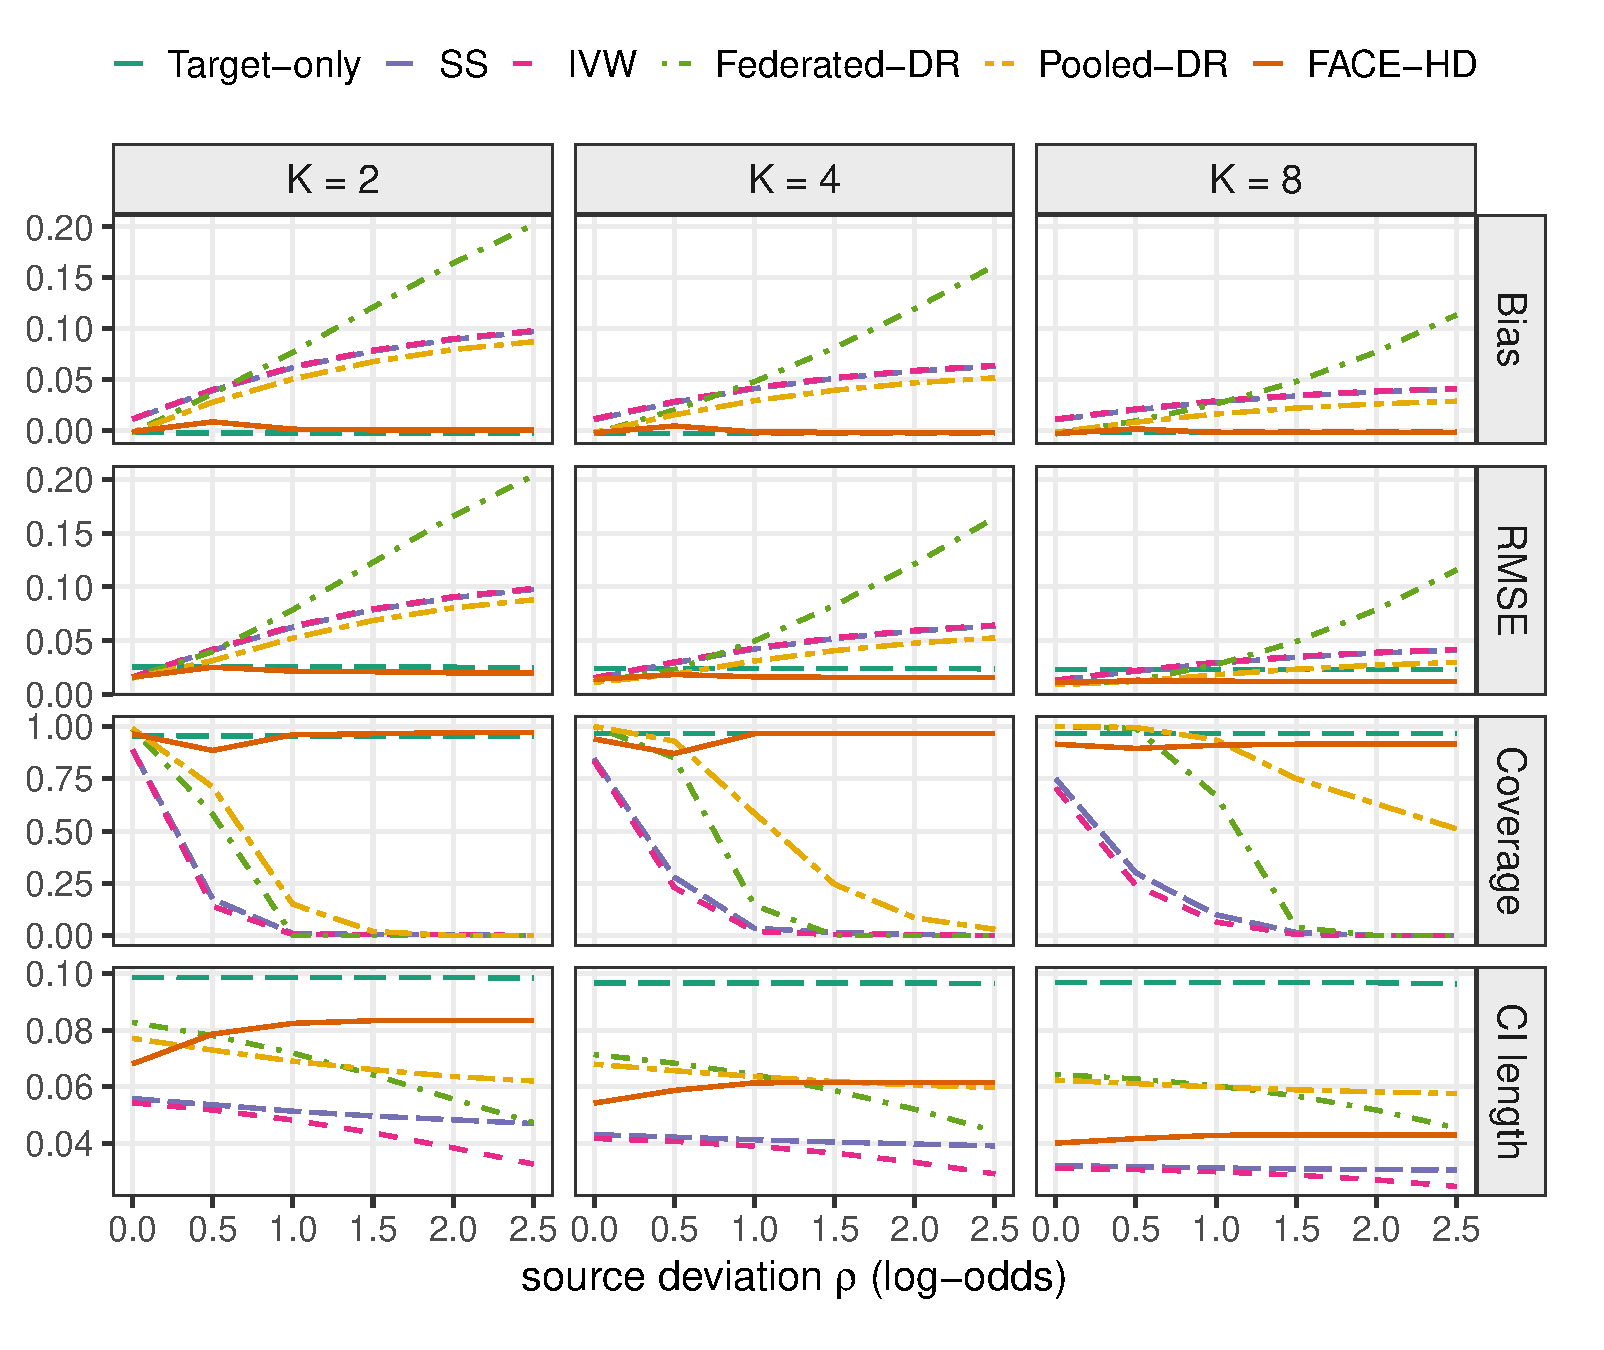
\includegraphics[width=\textwidth,height=0.62\textheight,keepaspectratio]{figures/sim_negtransfer_C2_p50.pdf}
\caption{Legacy treated-mean negative-transfer simulation, C(2), $p=50$. Panels show bias, RMSE,
$95\%$ coverage, and CI length for $\mu^1$ as the source deviation $\rho$ increases, with
columns for $K=2,4,8$ source sites. RoCE remains stable while the naive
aggregators lose coverage.}
\label{fig:sim_negtransfer_c2}
\end{figure}

\begin{figure}[t]
\centering
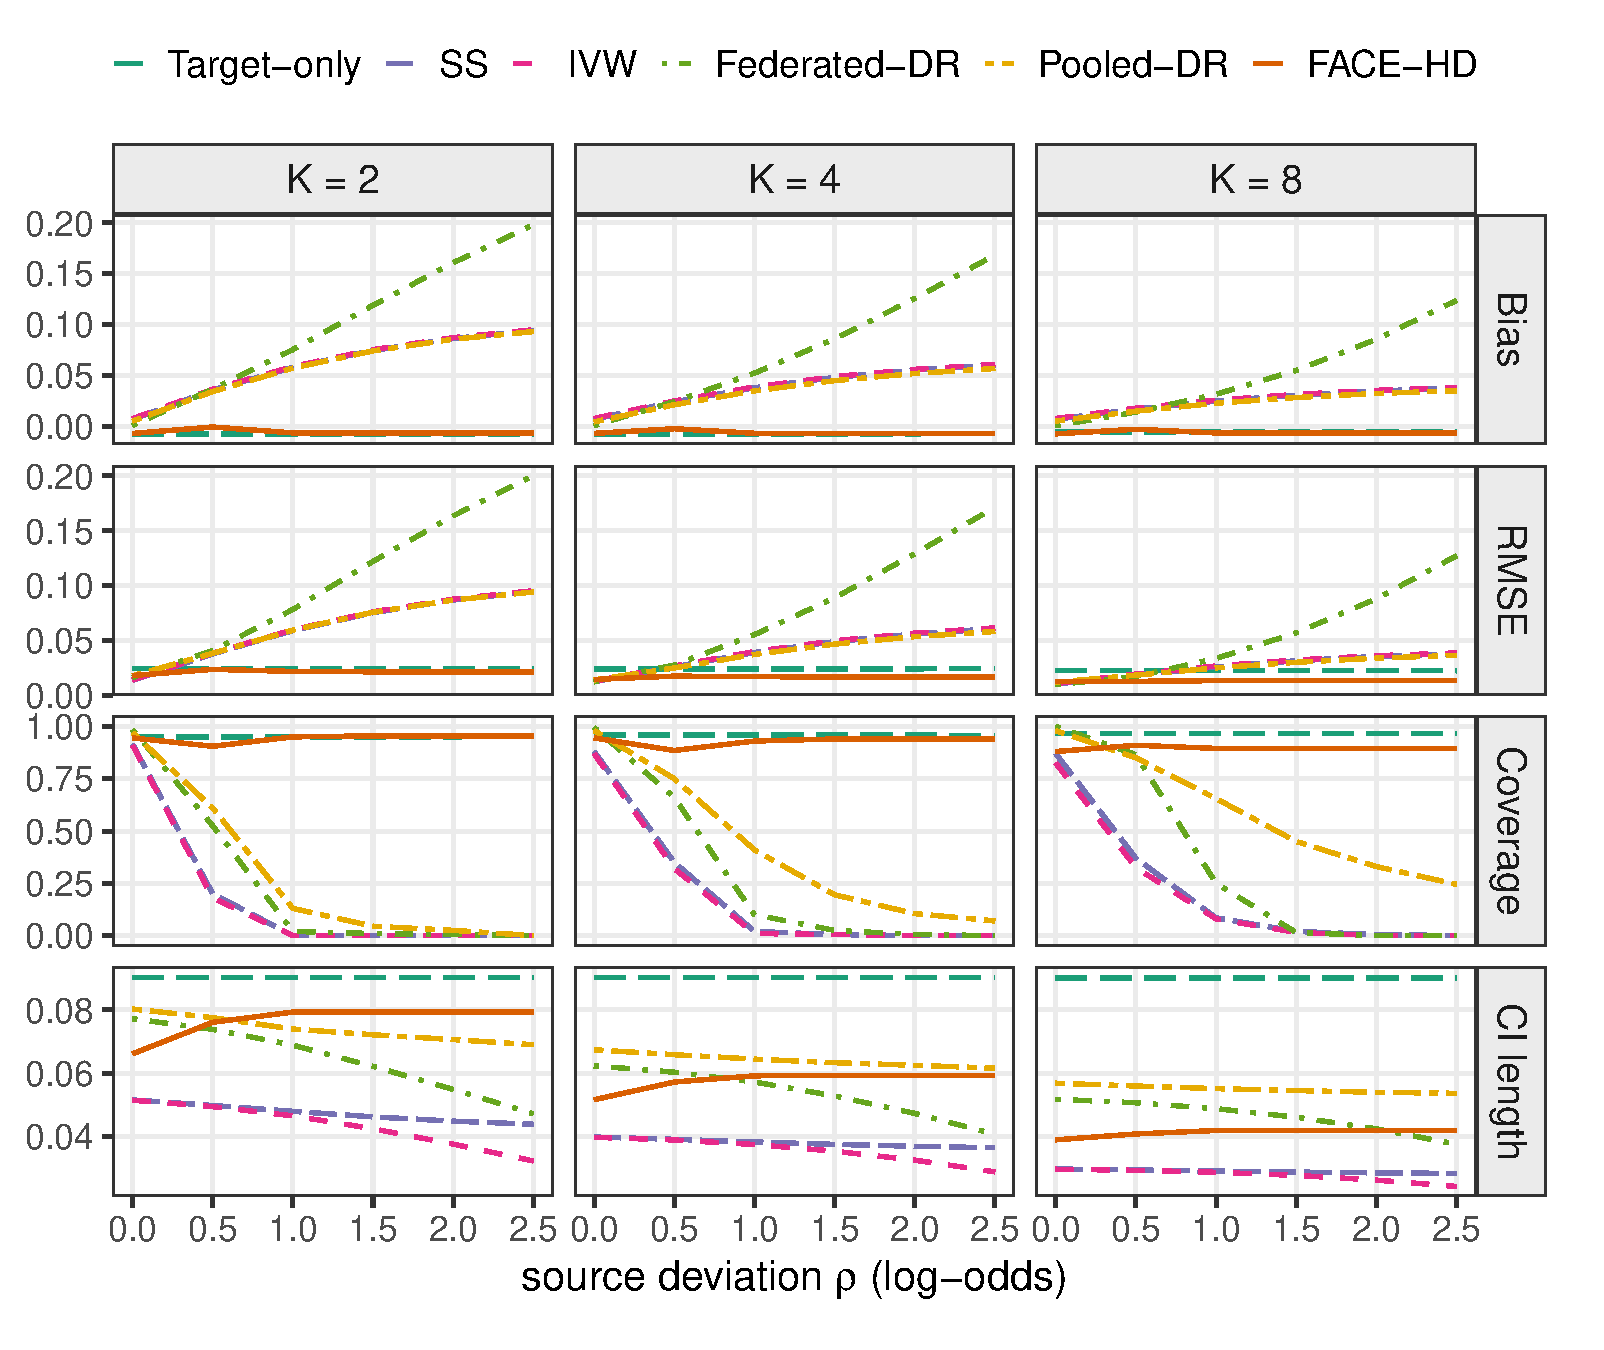
\includegraphics[width=\textwidth,height=0.62\textheight,keepaspectratio]{figures/sim_negtransfer_C3_p50.pdf}
\caption{Legacy treated-mean negative-transfer simulation, C(3), $p=50$. Same layout as
\cref{fig:sim_negtransfer_c2}; the site/propensity model is misspecified.}
\label{fig:sim_negtransfer_c3}
\end{figure}

\paragraph{Legacy lower-dimensional setting ($p=50$).}
The archived treated-mean study used the lower dimension $p=50$ (with
$n=1000$ observations per site, so $N=1000(K+1)$ in total). \Cref{fig:sim_negtransfer_p50}
shows C(1), which uses quadratic working bases for both nuisances. At
$\rho=0$, all sites share the conditional outcome mechanism and treatment
log-odds shift. A non-adaptive estimator may attain smaller finite-sample RMSE
when its variance reduction outweighs the modest covariate-shift-induced
differences in site-specific marginal effects, and no adaptation is needed. As $\rho$
increases, RoCE gives a substantially more stable bias--coverage tradeoff,
whereas SS, IVW, Federated-DR, and Pooled-DR become biased and lose coverage.
The C(2)--C(3) figures at $p=50$ display the same qualitative robustness
pattern, with some finite-sample undercoverage under C(3).

\begin{figure}[t]
\centering
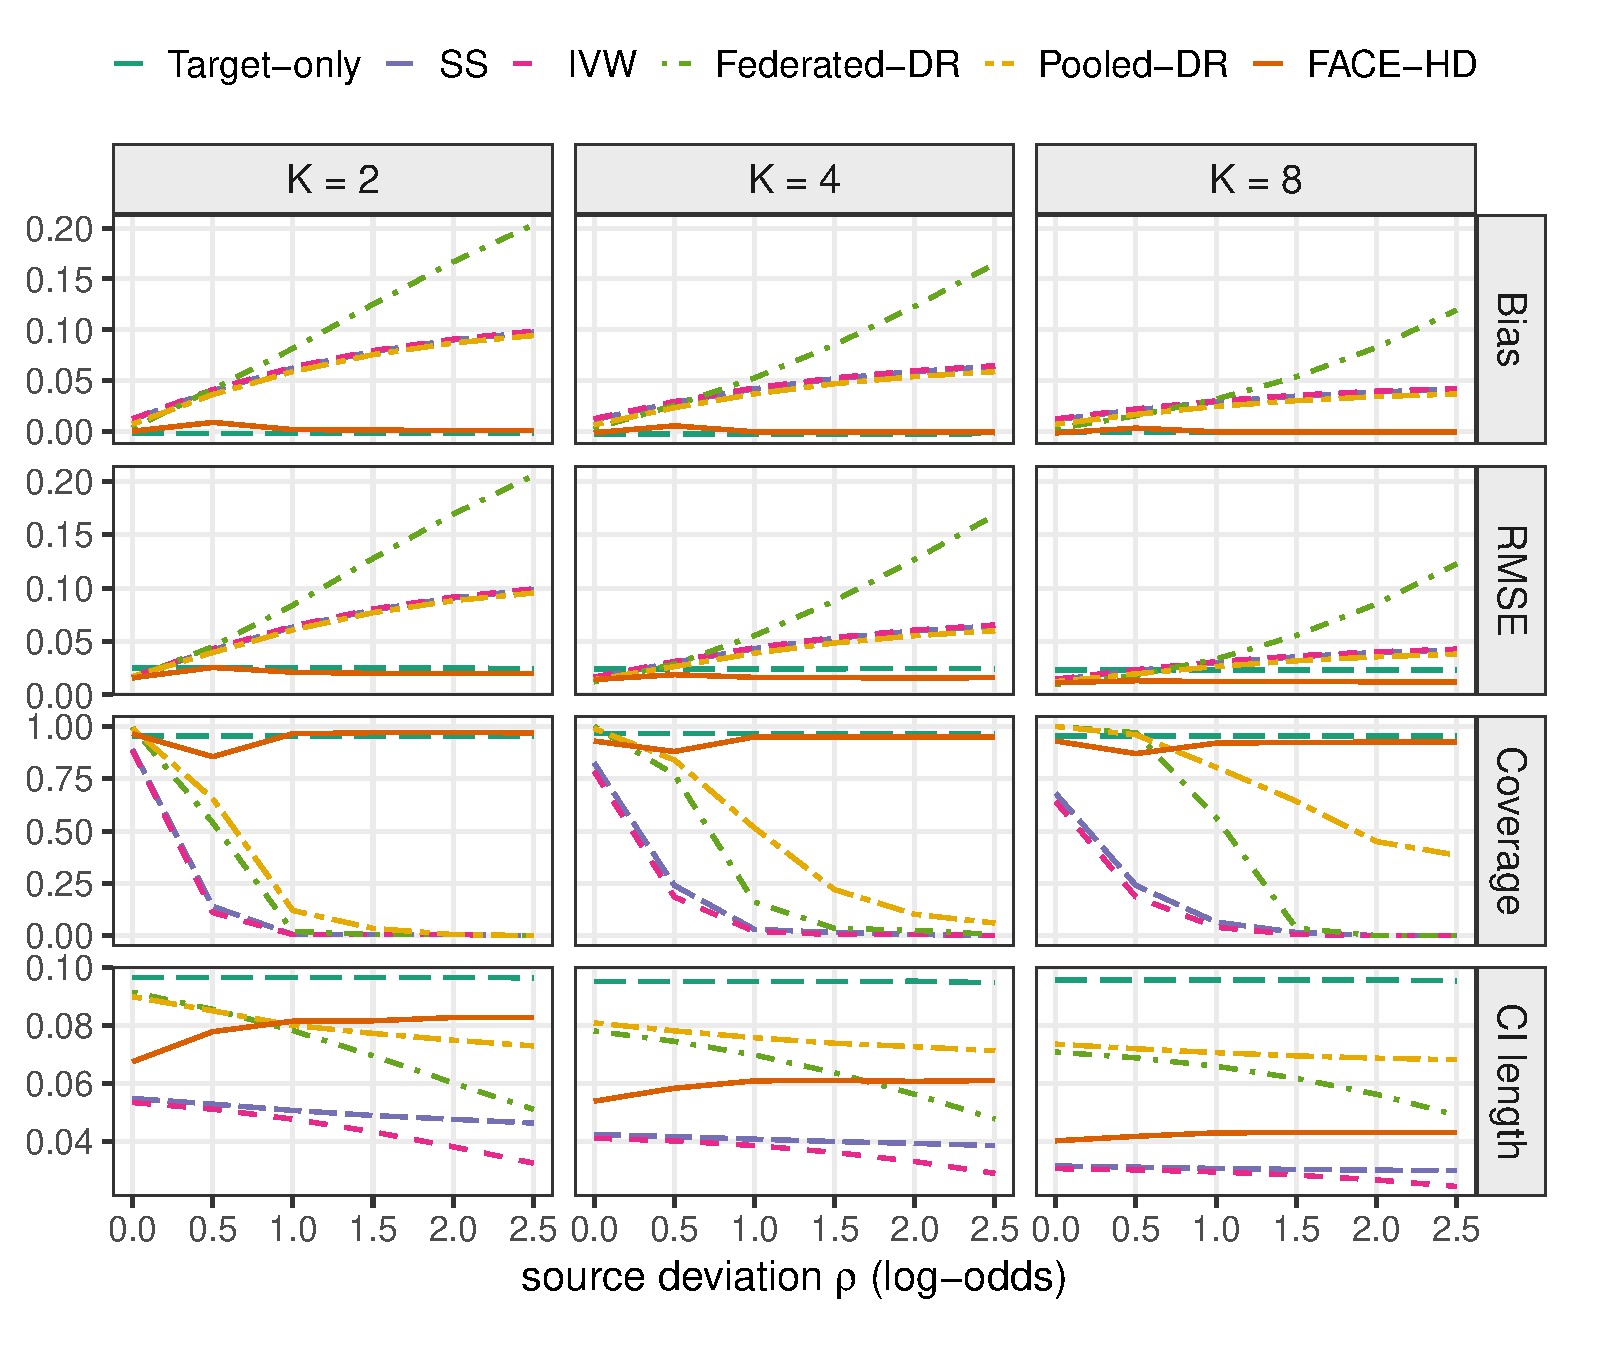
\includegraphics[width=\textwidth,height=0.62\textheight,keepaspectratio]{figures/sim_negtransfer_C1_p50.pdf}
\caption{Legacy treated-mean negative-transfer simulation, C(1), $p=50$. Same layout as
\cref{fig:sim_negtransfer_c2}; the conclusions match the $p=100$ case.}
\label{fig:sim_negtransfer_p50}
\end{figure}

\paragraph{One-round versus two-round.}
\Cref{fig:one_vs_two_round} compares the archived arm-wise TATE implementations
of one-round and two-round RoCE in a continuous-outcome setting where the sources remain mean-compatible but their
conditional outcome models differ in shape from the target's---a source-specific
effect modification of strength $s$, centered so that each source's target-population
mean treatment effect is unchanged. Across the full range of $s$ and at both
$p=10$ and $p=50$, the one-round and two-round curves track one another closely
in bias, RMSE, coverage, and interval length, and both are more efficient than
the target-only anchor. This is descriptive evidence rather than a formal
equivalence test: the archived cells contain 80 completed replicates at $p=10$
and 52--60 at $p=50$. It supports adopting the communication-light one-round version as the
default initialization; the two-round variant remains available as an alternative that relaxes the
target-initialization alignment condition. This diagnostic predates the
common-weight TATE aggregation and is retained without relabeling it as
the new estimator.

\begin{figure}[t]
\centering
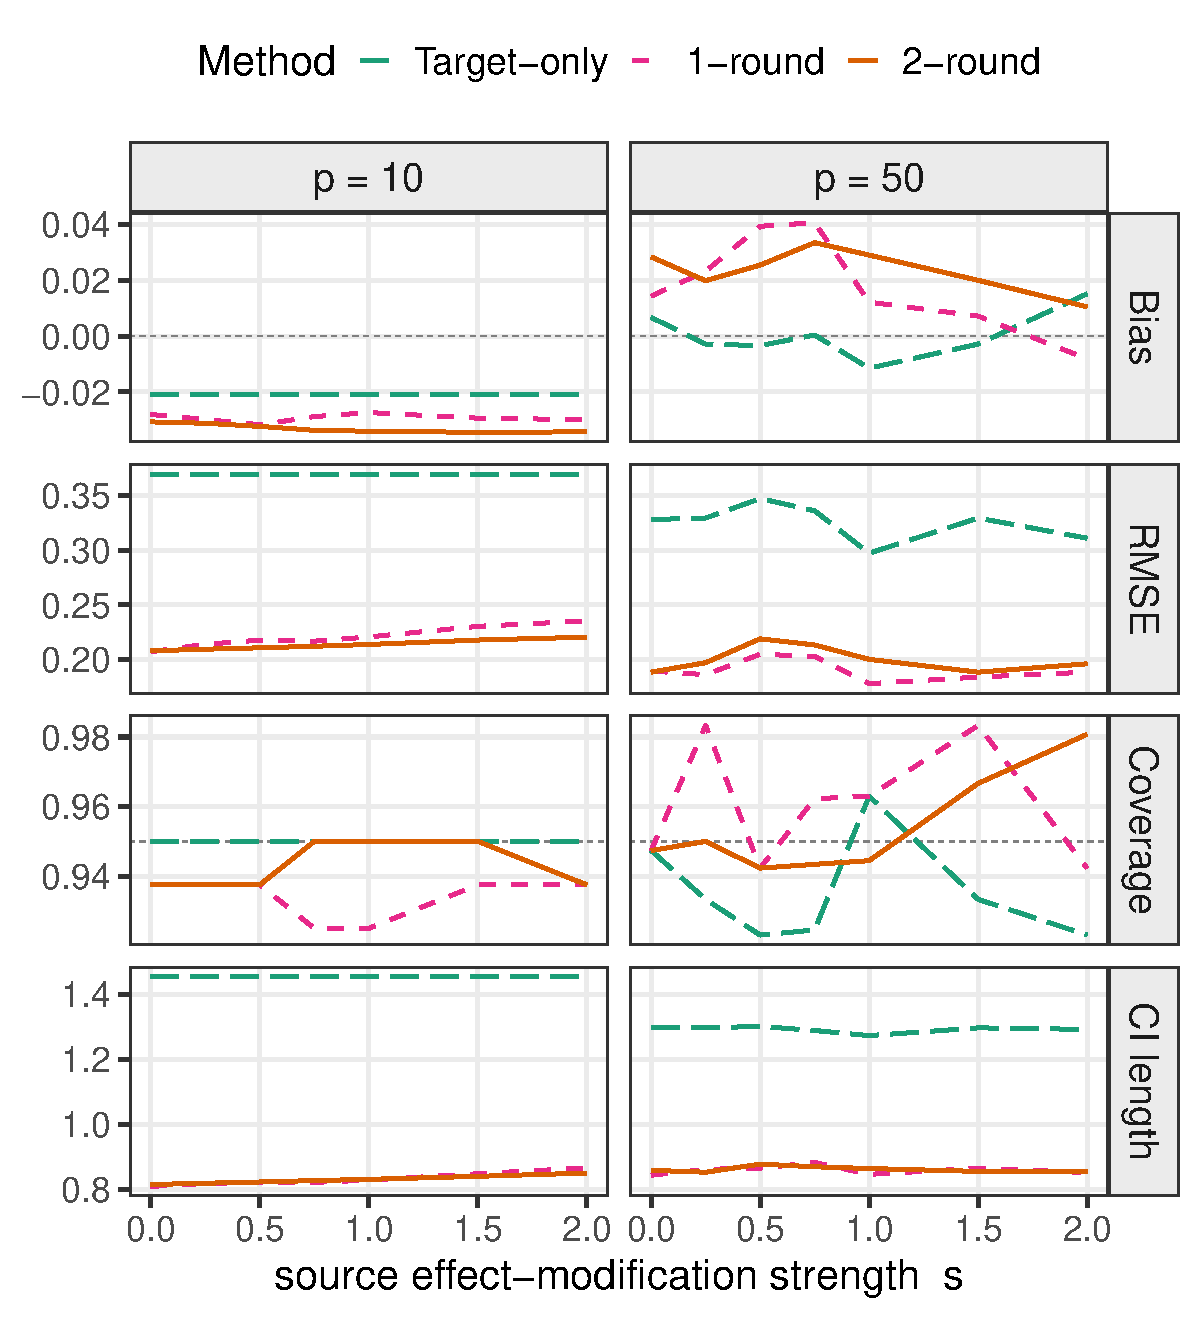
\includegraphics[width=0.9\linewidth]{figures/sim_2round_em_cont.pdf}
\caption{Archived one-round versus two-round arm-wise TATE RoCE for the
continuous-outcome experiment. Panels show TATE bias, RMSE, $95\%$ coverage,
and CI length as the effect-modification strength $s$ increases, for $p=10$
and $p=50$. Cells contain 80 completed replicates at $p=10$ and 52--60 at
$p=50$; the comparison is descriptive, and the two variants track closely.}
\label{fig:one_vs_two_round}
\end{figure}

%%%%%%%%%%%%%%%%%%%%%%%%%%%%%%%%%%%%%%%%%%%%%%%%%%%%%%%%%%%%%%%%%%%%%%%%%%%%%%%
%% SECTION 3: AGGREGATED ESTIMATOR PROOFS
%%%%%%%%%%%%%%%%%%%%%%%%%%%%%%%%%%%%%%%%%%%%%%%%%%%%%%%%%%%%%%%%%%%%%%%%%%%%%%%
\section{Aggregated Estimator: RoCE}
\label{supp:aggregation}

This section develops the aggregation theory for the TATE estimator in
the main manuscript. Arm-specific nuisances are fitted first, but their
influence-function components are contrasted before weights, Wald statistics,
or variances are calculated. The main result is \cref{thm:agg_roce}.

The proof proceeds in five steps. First, \cref{lem:agg_covariance_structure}
gives the quadratic TATE variance $L_\tau^*(\eta)$. Second,
\cref{lem:agg_variance_components} establishes uniform convergence of its
empirical analogue. Third, \cref{lem:agg_selection} proves TATE-level source
selection. Fourth, \cref{lem:agg_asymptotic_equivalence} makes estimated and
oracle weights first-order equivalent. Finally, the multisite CLT and Slutsky's
theorem give valid TATE inference.
 
\subsection{Setup and Notation for Aggregation}\label{supp:aggregation_setup}

Following \maincref{eq:direct_tate_aggregation}, aggregate the source-assisted
TATE estimators $\{\widehat{\tau}_{t,s_j}\}_{j=1}^K$ with the target-only TATE
$\widehat{\tau}_{ot}$ using one common weight vector.
Define the global sample size across all participating sites as
\[
N_{\mathrm{all}} := N_t + \sum_{j=1}^K N_{s_j},
\]
and assume $N_t/N_{\mathrm{all}} \to \rho_t^{\mathrm{all}} \in (0,1)$ and $N_{s_j}/N_{\mathrm{all}} \to \rho_{s_j}^{\mathrm{all}} \in (0,1)$ for each fixed $j$.

\textbf{Notation correspondence with the main manuscript:}
\begin{itemize}
    \item $\widehat{\tau}_{ot}=\widehat{\mu}_{ot}^1-\widehat{\mu}_{ot}^0$: target-only TATE;
    \item $\widehat{\tau}_{t,s_j}=\widehat{\mu}_{t,s_j}^1-\widehat{\mu}_{t,s_j}^0$: source-assisted TATE from $s_j$;
    \item $\varphi_{ot,i}^{\tau}=\varphi_{ot,i}^1-\varphi_{ot,i}^0$,
    $\zeta_{j,i}^{\tau}=\zeta_{j,i}^1-\zeta_{j,i}^0$, and
    $\xi_{j,i}^{\tau}=\xi_{j,i}^1-\xi_{j,i}^0$: treatment-contrast influence components.
\end{itemize}

The TATE estimator is
\[
\widehat{\tau}_{\mathrm{agg}}(\eta)
=\widehat{\tau}_{ot}
+\sum_{j=1}^K\eta_j
\left(\widehat{\tau}_{t,s_j}-\widehat{\tau}_{ot}\right).
\]

\begin{lemma}[Variance-Covariance Structure for Aggregation]\label{lem:agg_covariance_structure}
For each source site $s_j$, let $\varphi^\tau_{t,s_j,i}$ denote the
population influence contribution of $\widehat{\tau}_{t,s_j}$ under common
$\sqrt{N_{\mathrm{all}}}$ scaling, and let $\varphi^\tau_{ot,i}$ denote the
target-only TATE contribution. Write
\[
\varphi^\tau_{t,s_j,i}=\zeta^\tau_{j,i}+\xi^\tau_{j,i}.
\]
Then, for $j\neq k$,
\[
\Cov(\xi^\tau_j,\xi^\tau_k)=0,
\qquad
\Cov(\zeta^\tau_j,\xi^\tau_k)=0,
\qquad
\Cov(\varphi^\tau_{ot},\xi^\tau_k)=0,
\]
because these terms are based on disjoint source samples or on target-versus-source samples that are independent across sites. Consequently, all cross-site covariance terms arise only through the shared target component:
\[
\Cov(\varphi^\tau_{t,s_j},\varphi^\tau_{t,s_k})
=\Cov(\zeta^\tau_j,\zeta^\tau_k),
\qquad
\Cov(\varphi^\tau_{ot},\varphi^\tau_{t,s_j})
=\Cov(\varphi^\tau_{ot},\zeta^\tau_j).
\]
In particular, the population variance of the aggregated estimator can be written as a quadratic form
\[
L_\tau^*(\eta)=\eta^T H_\tau\eta
+\boldsymbol{d}_\tau^T\eta+c_\tau,
\]
where the off-diagonal entries of $H$ are induced entirely by the shared target sample.
\end{lemma}
\begin{proof}
The target sample is independent of every source sample, and source samples are
mutually independent. Taking an arm contrast changes neither this independence
nor the site on which a component is evaluated. Hence source--source and
target--source covariances vanish as displayed. Expanding the variance of
\[
\varphi^\tau_{\mathrm{agg}}(\eta)
=\varphi^\tau_{ot}
+\sum_{j=1}^K\eta_j
(\varphi^\tau_{t,s_j}-\varphi^\tau_{ot})
\]
then gives the stated quadratic representation, with off-diagonal terms coming solely from the shared target contribution.
\end{proof}

\begin{remark}[Relation to FACE as a special case]\label{rem:agg_face_special_case}
\cref{lem:agg_covariance_structure} is compatible with the covariance decomposition underlying \citet{han2025federated}. In particular, if the source-assisted estimators are specialized to the FACE construction and the nuisance structure is simplified to the corresponding low-dimensional setting, then the same argument shows that cross-source covariance is induced only by the shared target sample. Thus the FACE variance formula can be viewed as a special case of the present decomposition, whereas the current statement is written to accommodate the more general high-dimensional calibrated nuisance estimators used in RoCE.
\end{remark}

\subsection{Penalized Variance Estimation}\label{supp:aggregation_penalty}

Define the empirical TATE loss:
\[
\widehat{L}_\tau(\eta)
=N_{\mathrm{all}}\widehat{\Var}
\{\widehat{\tau}_{\mathrm{agg}}(\eta)\}
\]
which is a quadratic function of $\eta$ (equivalently, $N_{\mathrm{all}}$ times the variance expression in \maincref{eq:agg_penalized_objective} in the main manuscript):
\[
\widehat{L}_\tau(\eta)
=\eta^T\widehat H_\tau\eta+\widehat{\boldsymbol d}_\tau^T\eta
+\widehat c_\tau
\]
where every component is calculated after taking the arm contrast.

For the implemented two-level cross-fitting, let
$\widehat L_{\tau,-k}$ denote this objective calculated only from the outer
training sample $\mathcal T_k$, and let $\widehat\eta^{(-k)}$ be its penalized
minimizer. In the supporting arguments below, $\widehat L_\tau$ and
$\widehat\eta$ are shorthand for an arbitrary fixed outer fold's
$\widehat L_{\tau,-k}$ and $\widehat\eta^{(-k)}$. Since $K_f$ is fixed, every
$o_p(1)$ statement holds uniformly over $k\le K_f$. The final held-out
pseudo-value variance $\widehat V_\tau$ is a distinct finite-sample quantity;
both it and the foldwise training objectives evaluated at their minimizers
converge to $L_\tau^*(\eta_\tau^*)$.

\begin{lemma}[Consistency of Variance/Covariance Components]\label{lem:agg_variance_components}
Assume \cref{asmp:pairwise_data,asmp:pairwise_overlap,asmp:pairwise_nuisance}
for both arms, and let $K$ be fixed. Let
$H_\tau,\boldsymbol d_\tau,c_\tau$ denote the population analogues. Define
\[
a_N
\coloneqq
\max_{a\in\{0,1\}}\max_{j\le K}\max_{k\le K_f}
\left\{
\|\widehat{\boldsymbol{\alpha}}_{t,s_j}^{a,(-k)}
-\boldsymbol{\alpha}_{t,s_j}^{a,*}\|_2
+
\|\widehat{\boldsymbol{\gamma}}_{s_j,a}^{(-k)}
-\boldsymbol{\gamma}_{s_j,a}^*\|_2
\right\}
=o_p(1).
\]
Then:
\[
\|\widehat{H}_\tau-H_\tau\|_{\mathrm{op}}
+\|\widehat{\boldsymbol{d}}_\tau-\boldsymbol{d}_\tau\|_2
+|\widehat{c}_\tau-c_\tau|
=o_p(1),
\]
and consequently, for any fixed compact set $\mathcal{B}\subset\R^K$,
\[
\sup_{\eta\in\mathcal{B}}
|\widehat{L}_\tau(\eta)-L_\tau^*(\eta)|=o_p(1).
\]
If the products of the relevant influence-function components have uniformly bounded second moments, the empirical-averaging part is $O_p(N_{\mathrm{all}}^{-1/2})$, giving the sharper bound $O_p(N_{\mathrm{all}}^{-1/2})+O_p(a_N)$. This sharper rate is not needed for the RoCE oracle limit.
\end{lemma}
\begin{proof}
For readability in this proof only, suppress the subscript $\tau$ on
$\widehat H_\tau,H_\tau,\widehat{\boldsymbol d}_\tau,\boldsymbol d_\tau,
\widehat c_\tau,c_\tau,\widehat L_\tau$, and $L_\tau^*$.
We prove entrywise consistency and then convert to the stated matrix/vector norms using that $K$ is fixed.

\textbf{Step 1 (Generic moment form).}
Each element of $\widehat{H}$, $\widehat{\boldsymbol{d}}$ and $\widehat{c}$ is a (finite) linear combination of empirical averages of the form
\[
\widehat{M}_{r} \;=\; \frac{1}{N_r}\sum_{i\in\mathcal{D}_r} f(D_i;\widehat{\vartheta}^{(-\mathrm{fold}(i))}),
\qquad r\in\{t,s_1,\ldots,s_K\},
\]
where $f$ is a product of two empirical influence-function components (including the cross-site covariance terms computed on the \emph{same} target sample), and $\widehat{\vartheta}^{(-\mathrm{fold}(i))}$ denotes the cross-fitted nuisance estimate used to evaluate the fold containing $i$.
Let $M_r$ be the population analogue obtained by replacing the sample average with $\E_r[\cdot]$ and $\widehat{\vartheta}^{(-\mathrm{fold}(i))}$ with the population target $\vartheta^*$.

\textbf{Step 2 (Conditional LLN and plug-in stability).}
Partition the site-$r$ average by evaluation fold:
\[
\widehat M_r
=\sum_{k=1}^{K_f}\frac{N_{r,k}}{N_r}\widehat M_{r,k},
\qquad
\widehat M_{r,k}
=\frac{1}{N_{r,k}}\sum_{i\in\mathcal D_{r,k}}
f(D_i;\widehat\vartheta^{(-k)}).
\]
For each fixed $k$, conditional on $\mathcal D^{(-k)}$, the nuisance estimate
is fixed and the evaluation-fold summands in $\widehat M_{r,k}$ are
independent. The conditional weak law of large numbers therefore gives
\[
\widehat M_{r,k}
-\E_r[f(D;\widehat\vartheta^{(-k)})\mid\mathcal D^{(-k)}]
=o_p(1).
\]
Because $K_f$ is fixed, summing these foldwise statements gives
\[
\widehat M_r
-\sum_{k=1}^{K_f}\frac{N_{r,k}}{N_r}
\E_r[f(D;\widehat\vartheta^{(-k)})\mid\mathcal D^{(-k)}]
=o_p(1).
\]
This conditions on one fold's training sample at a time, rather than jointly
on the overlapping collection $\{\mathcal D^{(-k)}\}_{k=1}^{K_f}$. If the
products have uniformly bounded second moments, each foldwise empirical term
is $O_p(N_{r,k}^{-1/2})$, and the fixed weighted sum is
$O_p(N_r^{-1/2})$. \cref{asmp:pairwise_overlap}(b) gives the required uniform
integrability in a neighborhood of $\vartheta^*$.
Next, by \cref{asmp:pairwise_nuisance}(d), $\widehat{\vartheta}^{(-k)}\to_p \vartheta^*$, and by the same local $L_2$ stability argument used in \cref{lem:pairwise_bias_variance} (Part 2), the mapping $\vartheta\mapsto f(D;\vartheta)$ is locally $L_2$-Lipschitz. Therefore,
\[
\max_{1\le k\le K_f}
\left|
\E_r[f(D;\widehat{\vartheta}^{(-k)})\mid\mathcal D^{(-k)}]
-\E_r[f(D;\vartheta^*)]
\right|
=O_p(a_N),
\]
and combining the two displays yields $\widehat{M}_r-M_r=o_p(1)+O_p(a_N)=o_p(1)$.
Under the additional second-moment condition above, the empirical-averaging part is $O_p(N_r^{-1/2})$, hence $O_p(N_{\mathrm{all}}^{-1/2})$ under the site-ratio condition $N_r/N_{\mathrm{all}}\to\rho_r>0$.

\textbf{Step 3 (From entrywise to matrix/vector norms).}
Since $\widehat{H}$ has fixed dimension $K\times K$ and $\widehat{\boldsymbol{d}}$ has fixed dimension $K$, the preceding bound applies to each entry, hence
\[
\|\widehat{H}-H\|_{\mathrm{op}}
\le
C_K\max_{j,k}|\widehat{H}_{jk}-H_{jk}|
=o_p(1),
\qquad
\|\widehat{\boldsymbol{d}}-\boldsymbol{d}\|_2
\le
\sqrt{K}\max_j|\widehat{d}_j-d_j|
=o_p(1),
\]
Finally, $\widehat{c}$ is a finite linear combination of the same sample averages $\{\widehat{M}_r\}$ (coming from the constant terms in the variance expansion), so the same entrywise bound implies $|\widehat{c}-c|=o_p(1)$.

\textbf{Step 4 (Uniform convergence of the quadratic form).}
For $\eta$ in a fixed compact set $\mathcal{B}\subset\R^K$,
\[
|\widehat{L}(\eta)-L^*(\eta)|
\le
\|\widehat{H}-H\|_{\mathrm{op}}\|\eta\|_2^2 + \|\widehat{\boldsymbol{d}}-\boldsymbol{d}\|_2\|\eta\|_2 + |\widehat{c}-c|,
\]
and the right-hand side is $o_p(1)$ uniformly over $\eta\in\mathcal{B}$ because $\sup_{\eta\in\mathcal{B}}\|\eta\|_2<\infty$.
\end{proof}

The penalized objective uses the TATE-level truncated-Wald penalty. Recall
$\widehat L_\tau(\eta)=N_{\mathrm{all}}\widehat{\Var}
\{\widehat\tau_{\mathrm{agg}}(\eta)\}$:
\begin{equation}\label{eq:supp_agg_penalized_objective}
\widehat{\eta} = \arg\min_{\eta\in\mathbb R^K}
\left\{\widehat{L}_\tau(\eta)
+\sum_{j=1}^K(\lambda\widehat t_j^\tau-1)_+|\eta_j|\right\},
\qquad
\widehat t_j^\tau
\coloneqq
\frac{|\widehat\tau_{ot}-\widehat\tau_{t,s_j}|}
{\widehat{\mathrm{SE}}(\mathrm{disc}_j^\tau)},
\end{equation}
where $\mathrm{disc}_j^\tau=\widehat\tau_{ot}-\widehat\tau_{t,s_j}$ and
\[
\widehat{\mathrm{SE}}(\mathrm{disc}_j^\tau)^2
=
\frac{\widehat V_{ot}^\tau}{N_t}
+\frac{\widehat V_{t,s_j}^\tau}{N_t}
+\frac{\widehat V_{s_j}^\tau}{N_{s_j}}
-\frac{2\widehat C_{ot,s_j}^\tau}{N_t}
=
\widehat{\Var}(\widehat\tau_{t,s_j}-\widehat\tau_{ot}).
\]
Equivalently, the implementation minimizes the unscaled variance plus
$N_{\mathrm{all}}^{-1}\sum_j(\lambda\widehat t_j^\tau-1)_+|\eta_j|$.
This exact rescaling is tested in the codebase. The penalty is inactive when
$\widehat t_j^\tau\le1/\lambda$. The oracle-selection regime is
$1/\lambda\to\infty$ while
$1/\lambda=o(\sqrt{N_{\mathrm{all}}}b_{0,N}^\tau)$.

\begin{remark}[FACE-style validation for $\lambda$]\label{rem:agg_lambda_validation}
The main manuscript fixes the aggregation penalty-activation threshold at the locked pilot value $1/\lambda=1$ and does not tune it on the analyzed data. The FACE sample-splitting validation rule described here is an optional alternative for those who instead wish to tune $\lambda$ over a grid: for each outer evaluation fold, candidate weights are learned on inner-training summaries by solving the penalized aggregation problem, and these fixed weights are then evaluated on held-out inner-validation summaries through the pure validation-variance criterion. The penalty is used to construct each training-fold candidate but is not added again to its held-out validation score. This optional validation step is a finite-sample rule for choosing a stable point along the penalized aggregation path; it is not the same object as the nuisance-model cross-validation used for $\boldsymbol{\alpha}$ and $\boldsymbol{\gamma}$.
For the asymptotic arguments below, $\lambda=\lambda_N$ determines the Wald-significance penalty-activation threshold of \cref{eq:supp_agg_penalized_objective}: it may be deterministic or data-adaptive, provided it is measurable with respect to the outer training data and satisfies \cref{asmp:agg_regular}(b)--(c) (i.e.\ $1/\lambda_N \to \infty$ while $1/\lambda_N=o(\sqrt{N_{\mathrm{all}}}\,b_{0,N})$) with probability tending to one; it is \emph{not} a penalty parameter driven to infinity. Under fixed separation this condition is the simpler $\lambda_N\to0$ and $\lambda_N\sqrt{N_{\mathrm{all}}}\to\infty$. The inner validation construction preserves the cross-fitting independence needed for the influence-function expansion because the training summaries used to compute $\widehat{\eta}^{(-k,-m)}(\lambda)$, the validation summaries used to choose $\widehat{\lambda}^{(-k)}$, and the final outer evaluation fold $\mathcal{D}_k$ are separated. Consequently neither $\widehat{\lambda}^{(-k)}$ nor $\widehat{\eta}^{(-k)}$ uses the outer evaluation fold $\mathcal{D}_k$.
In the production implementation, the locked threshold $1/\lambda=1$
activates the penalty when $\widehat t_j^\tau>1$. Crossing this threshold
initiates soft shrinkage and is not interpreted as a stand-alone hypothesis
test or as guaranteed source exclusion.
\end{remark}

\begin{remark}[Soft-thresholding interpretation]\label{rem:agg_soft_threshold}
The penalty in \cref{eq:supp_agg_penalized_objective} is adaptive $\ell_1$.
For a diagonal Hessian of $\widehat L_\tau$, each coordinate minimizes
\[
\widehat{H}_{\tau,jj}\eta_j^2
+\widehat b_{\tau,j}\eta_j
+(\lambda\widehat t_j^\tau-1)_+|\eta_j|,
\qquad
\widehat b_{\tau,j}
\coloneqq
\frac{\partial\widehat L_\tau}{\partial\eta_j}\Big|_{\eta=0}
=
N_{\mathrm{all}}\,
\frac{2(\widehat C_{ot,s_j}^\tau-\widehat V_{ot}^\tau)}{N_t},
\]
where $\widehat b_{\tau,j}=O_p(1)$ is the asymptotic-variance gradient at
$\eta=0$. Completing the square yields the explicit solution
\[
\widehat{\eta}_j
=
\mathrm{SoftThreshold}\!\left(
\eta_j^{\mathrm{OLS}},
\frac{(\lambda\widehat t_j^\tau-1)_+}{2\widehat H_{\tau,jj}}
\right),
\qquad
\eta_j^{\mathrm{OLS}}
\coloneqq-\frac{\widehat b_{\tau,j}}{2\widehat H_{\tau,jj}},
\]
where $\eta_j^{\mathrm{OLS}}$ is the unpenalized variance-minimizing coordinate. Equivalently, the KKT selection rule is
\[
\widehat{\eta}_j = 0
\quad\Longleftrightarrow\quad
|\widehat b_{\tau,j}|\le(\lambda\widehat t_j^\tau-1)_+,
\]
with the analogous coupled KKT conditions for a non-diagonal Hessian.
\end{remark}

\subsection{Informative Source Indices}\label{supp:aggregation_informative_indices}

For each source, write
$\mu_{t,s_j}^{a,*}=\operatorname{plim}\widehat\mu_{t,s_j}^a$. Define the
TATE-compatible source set
\[
\mathcal{J}_\tau^*
=\{j:\mu_{t,s_j}^{1,*}-\mu_{t,s_j}^{0,*}=\tau\}
=\{j:\operatorname{plim}\widehat\tau_{t,s_j}=\tau\}.
\]
Define the oracle-restricted space:
\[
\mathbb{R}_{\mathcal{J}_\tau^*}
:=\{\eta\in\mathbb{R}^K:\eta_j=0
\text{ for all }j\notin\mathcal{J}_\tau^*\}.
\]
Let $\eta_\tau^*$ be the oracle TATE weights:
\[
\eta_\tau^*
=\arg\min_{\eta\in\mathbb{R}_{\mathcal{J}_\tau^*}}
L_\tau^*(\eta),\qquad
L_\tau^*(\eta)
=\Var\{\sqrt{N_{\mathrm{all}}}
(\widehat\tau_{\mathrm{agg}}(\eta)-\tau)\}.
\]

\begin{assumption}[Aggregation Regularity]\label{asmp:agg_regular}
Assume:
\begin{enumerate}[label=(\alph*),leftmargin=*]
    \item \emph{(Compatible sources and global curvature)}
    The set $\mathcal{J}_\tau^*$ is non-empty. The quadratic objective
    $L_\tau^*$ has a positive-definite Hessian on $\mathbb R^K$, with minimum
    eigenvalue bounded away from zero. Hence $L_\tau^*$ is coercive and has
    a finite unique minimizer on every coordinate subspace, including
    $\mathbb R_{\mathcal J_\tau^*}$.
    \item \emph{(Separation / ``$\beta$-min'' for biased sites)} Define
    \[
    b_{0,N}^\tau
    \coloneqq
    \min_{j\notin\mathcal{J}_\tau^*}
    |\operatorname{plim}(\widehat\tau_{t,s_j})-\tau|.
    \]
    Assume $b_{0,N}^\tau\sqrt{N_{\mathrm{all}}}\to\infty$ and that the asymptotic variance of each candidate TATE discrepancy $\sqrt{N_{\mathrm{all}}}\{\widehat\tau_{t,s_j}-\widehat\tau_{ot}\}$ is bounded away from zero.
    \item \emph{(Threshold rate)} The penalty-activation threshold satisfies
    \[
    \lambda \to 0,
    \qquad
    \lambda\sqrt{N_{\mathrm{all}}}b_{0,N}^\tau\to\infty,
    \]
    equivalently $1/\lambda=o(\sqrt{N_{\mathrm{all}}}b_{0,N}^\tau)$
    while $1/\lambda\to\infty$.
    \item \emph{(Fixed source set)} The number of source sites $K$ is fixed.
    \item \emph{(Compatible-source contrast expansion)} For every
    $j\in\mathcal J_\tau^*$, the centered contrast satisfies
    \[
    \sqrt{N_{t,s_j}}\left[
    \{\widehat\mu_{t,s_j}^1-\mu_{t,s_j}^{1,*}\}
    -\{\widehat\mu_{t,s_j}^0-\mu_{t,s_j}^{0,*}\}
    \right]
    =\frac{1}{\sqrt{N_{t,s_j}}}\sum_i
    \varphi_{t,s_j,i}^\tau+o_p(1),
    \]
    with the corresponding multisite scaling, a centered finite-variance
    influence function, and the uniform foldwise version used by the
    cross-fitted estimator. Separate application of
    \cref{thm:pairwise_mu1,thm:pairwise_mu0} is sufficient. If compatibility
    instead arises only because the two arm-specific pseudo-limit biases
    cancel, this contrast expansion is an additional assumption.
\end{enumerate}
\end{assumption}

If $\lambda$ is selected over a pre-specified sensitivity grid, the separation
and threshold-window conditions are interpreted as high-probability conditions
on the selected sequence. The primary implementation instead fixes
$1/\lambda=1$ before examining the outer evaluation fold.  The oracle support
recovery and single normal limit stated below therefore concern the
rate-indexed sequence in \cref{asmp:agg_regular}(c); they are not asserted for
the fixed-cutoff implementation without an additional fixed-threshold
argument.

\begin{remark}[When separation fails / local alternatives]\label{rem:agg_weak_bias}
\cref{asmp:agg_regular}(b) is used only for support recovery. Under local
TATE alternatives $b_{0,N}^\tau=O(N_{\mathrm{all}}^{-1/2})$, exact selection
can fail because $\widehat t_j^\tau$ remains $O_p(1)$. The added first-order
bias is controlled by
\[
\left|\sum_{j\notin\mathcal{J}_\tau^*}\eta_j
\{\operatorname{plim}(\widehat\tau_{t,s_j})-\tau\}\right|,
\]
which is negligible when the included TATE deviations are
$o(N_{\mathrm{all}}^{-1/2})$.
\end{remark}

\subsection{Connection to the Original FACE Squared-Discrepancy Objective}\label{supp:original_face_squared_objective}

The main RoCE estimator uses the truncated-Wald objective in \cref{eq:supp_agg_penalized_objective}. This subsection records the direct analogue of the original FACE adaptive-aggregation objective \citep[Equation~(11)]{han2025federated}, which uses the raw squared discrepancy rather than the studentized Wald statistic. With the notation of \cref{supp:aggregation_informative_indices}, define
\begin{equation}\label{eq:supp_face_squared_objective}
\widehat{\eta}_{\mathrm{sq}}
=
\arg\min_{\eta\in\mathbb R^K}
\left\{
\widehat{L}_\tau(\eta)
+
\lambda_{\mathrm{sq},N}\sum_{j=1}^K
|\eta_j|\,(\mathrm{disc}_j^\tau)^2
\right\},
\qquad
\mathrm{disc}_j^\tau
=
\widehat\tau_{ot}-\widehat\tau_{t,s_j},
\end{equation}
where $\widehat L_\tau(\eta)$ is the same rescaled TATE-variance objective used
in \cref{eq:supp_agg_penalized_objective}.

The oracle argument is the same as the proof of \cref{lem:agg_selection}, but the rate window is different. Suppose \crefrange{asmp:pairwise_data}{asmp:pairwise_nuisance} hold and that the global-curvature and fixed-$K$ parts of \cref{asmp:agg_regular}(a),(d) hold. If the raw-discrepancy tuning parameter satisfies
\begin{equation}\label{eq:supp_face_squared_rates}
\lambda_{\mathrm{sq},N}\to\infty,
\qquad
\lambda_{\mathrm{sq},N}=o\!\left(N_{\mathrm{all}}^{1/2}\right),
\qquad
\lambda_{\mathrm{sq},N}(b_{0,N}^\tau)^2\to\infty,
\end{equation}
then the squared-discrepancy objective has the same oracle-selection behavior:
\[
P\!\left(\widehat{\eta}_{\mathrm{sq},j}=0\
\text{ for all }j\notin\mathcal{J}_\tau^*\right)\to1,
\qquad
\|\widehat{\eta}_{\mathrm{sq},\mathcal{J}_\tau^*}
-\eta_{\tau,\mathcal{J}_\tau^*}^*\|_2=o_p(1).
\]
For each $j\in\mathcal{J}_\tau^*$, the two arm expansions imply
$\mathrm{disc}_j^\tau=O_p(N_{\mathrm{all}}^{-1/2})$, hence
\[
\lambda_{\mathrm{sq},N}(\mathrm{disc}_j^\tau)^2
=
O_p(\lambda_{\mathrm{sq},N}/N_{\mathrm{all}})
=
o_p(N_{\mathrm{all}}^{-1/2}),
\]
so the penalty is negligible on the oracle subspace. For each
$j\notin\mathcal{J}_\tau^*$,
$|\mathrm{disc}_j^\tau|\ge b_{0,N}^\tau/2$ w.p.a.1; therefore
\[
\lambda_{\mathrm{sq},N}(\mathrm{disc}_j^\tau)^2
\ge
\tfrac14\lambda_{\mathrm{sq},N}(b_{0,N}^\tau)^2
\to\infty
\qquad\text{w.p.a.1.}
\]
As in \cref{lem:agg_selection}, coercivity first gives
$\|\widehat{\eta}_{\mathrm{sq}}\|_2=O_p(1)$, and the gradient of the quadratic
variance part is therefore $O_p(1)$ along the segment joining the optimizer
to its coordinate-zero competitor. The diverging adaptive penalty makes that
competitor strictly favorable unless
$\widehat{\eta}_{\mathrm{sq},j}=0$, forcing zero weights for biased sources.

Under fixed TATE separation, this reduces to the original FACE scaling
$\lambda_{\mathrm{sq},N}\to\infty$ and
$\lambda_{\mathrm{sq},N}=o(N_{\mathrm{all}}^{1/2})$. The truncated-Wald
objective needs only the weaker studentized TATE separation in
\cref{asmp:agg_regular}.

\subsection{Aggregation Main Results}\label{supp:aggregation_main_results}

For later use in the aggregation proofs, we restate the pairwise input result that is repeatedly invoked below.

\begin{theoremRep}{thm:pairwise_mu1}
Suppose \cref{asmp:pairwise_data,asmp:pairwise_overlap,asmp:pairwise_nuisance} hold. Assume $\vartheta^*$ is the unique population target pair induced by the calibrated losses under the alignment condition in \cref{asmp:pairwise_nuisance}(c), implying \cref{lem:pairwise_orthogonality} holds. If further, at least one nuisance model (outcome or weighting) is correctly specified in the sense of \cref{lem:pairwise_identification_dr} (so $\mu^1(\vartheta^*)=\mu^1$), the calibrated nuisance sparsities satisfy
\[
\frac{(s_\alpha+s_\gamma)^2 \log^2(p)}{N} \longrightarrow 0,
\]
and $V^*_{t,s}>0$, then the cross-fitted estimator is asymptotically normal. Here $s_\alpha$ and $s_\gamma$ denote the calibrated sparsities from \cref{def:pairwise_sparsity}:
\[
\sqrt{N}\,\big(\widehat{\mu}^{1,\mathrm{CF}}_{t,s} - \mu^1\big)
\;\xrightarrow{d}\; \mathcal{N}\!\big(0,\,V^*_{t,s}\big).
\]
If the initial nuisance estimators enter the two-level algorithm separately from the calibrated update, their stochastic effect is absorbed through \cref{asmp:pairwise_nuisance}(c)--(d). The finite-sample KKT perturbation from the $\ell_1$ penalties is likewise absorbed in these nuisance-rate conditions and is $o_p(N^{-1/2})$ under the stated sparsity scaling.
\end{theoremRep}

\begin{theorem}[Asymptotic Normality of RoCE TATE]\label{thm:agg_roce}
Suppose the pairwise assumptions hold and
\cref{asmp:agg_regular} holds. For $j\in\mathcal J_\tau^*$, let
$N_{t,s_j}=N_t+N_{s_j}$ and let $s_{\mathrm{tot},j}$ bound the combined
arm-specific nuisance sparsity. If
\[
\max_{j\in\mathcal{J}_\tau^*}
\frac{s_{\mathrm{tot},j}^2\log^2(p)}{N_{t,s_j}}\to0,
\]
and $L_\tau^*(\eta_\tau^*)>0$, then
\[
\sqrt{N_{\mathrm{all}}}
(\widehat\tau_{\mathrm{agg}}-\tau)
\xrightarrow{d}
\mathcal N\{0,L_\tau^*(\eta_\tau^*)\}.
\]
Moreover, the within-site-centered pseudo-value estimator in
\maincref{eq:tate_federated_variance} is consistent:
\[
\widehat V_\tau\xrightarrow{p}L_\tau^*(\eta_\tau^*),
\]
while, uniformly over the fixed outer folds,
$\widehat L_{\tau,-k}\{\widehat\eta^{(-k)}\}
\xrightarrow{p}L_\tau^*(\eta_\tau^*)$; these two estimators need not be
numerically identical in finite samples. Furthermore,
\[
\max_{k\le K_f}
\|\widehat\eta^{(-k)}-\eta_\tau^*\|_2=o_p(1),
\qquad
P\!\left(\widehat\eta_j^{(-k)}=0\ \text{for every }
j\notin\mathcal J_\tau^*,\ k\le K_f\right)\to1,
\]
and
\[
\sqrt{\frac{N_{\mathrm{all}}}{\widehat V_\tau}}
(\widehat\tau_{\mathrm{agg}}-\tau)
\xrightarrow{d}\mathcal N(0,1).
\]
\end{theorem}

\begin{proposition}[TATE Efficiency Gain]\label{prop:agg_efficiency}
Under the conditions of \cref{thm:agg_roce}, RoCE TATE is
asymptotically at least as efficient as target-only TATE:
\[
L_\tau^*(\eta_\tau^*)\le L_\tau^*(0)
=V_{\tau,\mathrm{target}},
\]
with strict inequality whenever there exists $j\in\mathcal{J}_\tau^*$ such that
\[
\Var(\varphi^\tau_{t,s_j}-\varphi^\tau_{ot})>0
\quad\text{and}\quad
\Cov(\varphi^\tau_{ot},
\varphi^\tau_{t,s_j}-\varphi^\tau_{ot})\ne0.
\]
\end{proposition}

\subsection{Aggregation Supporting Lemmas}\label{supp:aggregation_supporting_lemmas}

To keep the remaining proofs readable, use the generic shorthand
\[
\theta=\tau,\quad
\widehat\theta_{ot}=\widehat\tau_{ot},\quad
\widehat\theta_{t,s_j}=\widehat\tau_{t,s_j},\quad
\widehat\theta_{\mathrm{agg}}=\widehat\tau_{\mathrm{agg}},\quad
\mathcal J^*=\mathcal J_\tau^*,\quad
\eta^*=\eta_\tau^*,\quad
L^*=L_\tau^*,
\]
and suppress the superscript $\tau$ on the treatment-contrast influence
components. Thus every object in the supporting lemmas below is TATE-level.

\begin{lemma}[Influence Function Representation]\label{lem:agg_if}
Under \crefrange{asmp:pairwise_data}{asmp:pairwise_nuisance} and
\cref{asmp:agg_regular}(a),(e), the aggregated estimator admits the
asymptotic linear representation:
\[
\sqrt{N_{\mathrm{all}}}
\{\widehat\theta_{\mathrm{agg}}(\eta^*)-\theta\}
=\frac{1}{\sqrt{N_{\mathrm{all}}}}
\sum_{i=1}^{N_{\mathrm{all}}}\varphi_{\mathrm{agg},i}(\eta^*)+o_p(1)
\]
where $\varphi_{\mathrm{agg},i}(\eta^*)$ is the aggregated influence function:
\[
\varphi_{\mathrm{agg},i}(\eta^*) = \left(1-\sum_{j\in\mathcal{J}^*}\eta_j^*\right)\varphi_{ot,i} + \sum_{j\in\mathcal{J}^*}\eta_j^* \varphi_{t,s_j,i},
\]
with $\varphi_{t,s_j,i}$ denoting the (rescaled) IF contribution of source-assisted estimator $j$ under $\sqrt{N_{\mathrm{all}}}$ scaling.
\textbf{Convention:} Each $\varphi_{ot,i}$ (resp.\ $\varphi_{t,s_j,i}$) is understood as zero for observations not in the target data $\mathcal{D}_t$ (resp.\ not in $\mathcal{D}_t\cup\mathcal{D}_{s_j}$), and includes the constant rescaling needed to convert its natural $\sqrt{N_t}$ (resp.\ $\sqrt{N_{t,s_j}}$) linear representation into the common $\sqrt{N_{\mathrm{all}}}$ scaling.
\end{lemma}

\begin{proof}
By the compatible-source contrast expansion in
\cref{asmp:agg_regular}(e)---which follows by applying the pairwise expansion
to both arms when they are separately identified---for every
$j\in\mathcal J^*$,
\[
\sqrt{N_{t,s_j}}
\{\widehat\theta_{t,s_j}
-\operatorname{plim}(\widehat\theta_{t,s_j})\}
=\frac{1}{\sqrt{N_{t,s_j}}}
\sum_{i=1}^{N_{\mathrm{all}}}\bar\varphi_{t,s_j,i}+o_p(1),
\]
where $\bar{\varphi}_{t,s_j,i}$ is understood as zero for observations not in $\mathcal{D}_t\cup\mathcal{D}_{s_j}$. Since $N_{t,s_j}/N_{\mathrm{all}}\to c_j\in(0,1)$, the above is equivalent to
\[
\sqrt{N_{\mathrm{all}}}
\{\widehat\theta_{t,s_j}
-\operatorname{plim}(\widehat\theta_{t,s_j})\}
=\frac{1}{\sqrt{N_{\mathrm{all}}}}
\sum_{i=1}^{N_{\mathrm{all}}}\varphi_{t,s_j,i}+o_p(1)
\]
for a rescaled IF $\varphi_{t,s_j,i}$. The target-only estimator has the analogous form:
\[
\sqrt{N_{\mathrm{all}}}(\widehat\theta_{ot}-\theta)
=\frac{1}{\sqrt{N_{\mathrm{all}}}}
\sum_{i=1}^{N_{\mathrm{all}}}\varphi_{ot,i}+o_p(1).
\]
For $j\in\mathcal J^*$,
$\operatorname{plim}(\widehat\theta_{t,s_j})=\theta$.

By linearity, the aggregated estimator with fixed $\eta = \eta^*$ satisfies:
\[
\sqrt{N_{\mathrm{all}}}
\{\widehat\theta_{\mathrm{agg}}(\eta^*)-\theta\}
=\frac{1}{\sqrt{N_{\mathrm{all}}}}
\sum_{i=1}^{N_{\mathrm{all}}}\varphi_{\mathrm{agg},i}(\eta^*)+o_p(1).
\]
The remainder remains $o_p(1)$ because $K$ is fixed.
\end{proof}

\begin{lemma}[Selection Consistency]\label{lem:agg_selection}
Under \crefrange{asmp:pairwise_data}{asmp:pairwise_nuisance} and \cref{asmp:agg_regular}, the penalized estimator $\widehat{\eta}$ from \cref{eq:supp_agg_penalized_objective} satisfies:
\begin{enumerate}
    \item \textbf{(Oracle-subspace consistency)} $\|\widehat{\eta} - \eta^*\|_2 = o_p(1)$
    \item \textbf{(Selection)} $\widehat{\eta}_j = 0$ for all $j \notin \mathcal{J}^*$ with probability approaching 1.
\end{enumerate}
\end{lemma}

\begin{proof}
We give a self-contained argument; it parallels the FACE proof in \citet{han2025federated} (Lemma S5) but the objective here is an explicit quadratic form.
Recall $\widehat{L}(\eta)=\eta^T\widehat{H}\eta+\widehat{\boldsymbol{d}}^T\eta+\widehat{c}$ and its population analogue $L^*(\eta)=\eta^TH\eta+\boldsymbol{d}^T\eta+c$.

\textbf{Part 1 (Consistency on the oracle subspace).}
Define the oracle-restricted estimator
\[
\widetilde{\eta} \;=\; \arg\min_{\eta\in\mathbb{R}_{\mathcal{J}^*}}
\left\{\widehat L(\eta)
+\sum_{j=1}^K(\lambda\widehat t_j^\tau-1)_+|\eta_j|\right\}.
\]
For $j\in\mathcal J^*$,
$\mathrm{disc}_j^\tau=\widehat\theta_{ot}-\widehat\theta_{t,s_j}
=O_p(N_{\mathrm{all}}^{-1/2})$ and
$\widehat t_j^\tau=O_p(1)$. Under $1/\lambda\to\infty$, the penalty is zero
on every oracle coordinate w.p.a.1, so $\widetilde\eta$ coincides with the
unpenalized TATE-variance minimizer on $\mathbb R_{\mathcal J^*}$.

Next, by \cref{lem:agg_variance_components}, the quadratic coefficients satisfy $\|\widehat{H}-H\|_{\mathrm{op}}=o_p(1)$ and $\|\widehat{\boldsymbol{d}}-\boldsymbol{d}\|_2=o_p(1)$.
Let $H_{\mathcal{J}^*}$ and $\widehat{H}_{\mathcal{J}^*}$ denote the principal submatrices corresponding to $\mathcal{J}^*$, and similarly let $\boldsymbol{d}_{\mathcal{J}^*}$ and $\widehat{\boldsymbol{d}}_{\mathcal{J}^*}$ denote the corresponding subvectors.
Because $K$ is fixed, $H_{\mathcal{J}^*}$ is a fixed-dimensional positive definite matrix by the global-curvature condition, hence $\|H_{\mathcal{J}^*}^{-1}\|_{\mathrm{op}}<\infty$ and $\|\widehat{H}_{\mathcal{J}^*}^{-1}\|_{\mathrm{op}}=O_p(1)$.
More explicitly, by Weyl's inequality and \cref{lem:agg_variance_components}, $\lambda_{\min}(\widehat{H}_{\mathcal{J}^*})\ge \lambda_{\min}(H_{\mathcal{J}^*}) - \|\widehat{H}_{\mathcal{J}^*}-H_{\mathcal{J}^*}\|_{\mathrm{op}}$, which is bounded away from 0 w.p.a.1, so $\widehat{H}_{\mathcal{J}^*}$ is invertible and $\|\widehat{H}_{\mathcal{J}^*}^{-1}\|_{\mathrm{op}}=O_p(1)$.
Because the penalty is zero on the oracle subspace w.p.a.1 and both quadratic
objectives are coercive and strictly convex there, their unconstrained
minimizers satisfy the first-order conditions
$2\widehat{H}_{\mathcal{J}^*}\eta + \widehat{\boldsymbol{d}}_{\mathcal{J}^*}=0$ and $2H_{\mathcal{J}^*}\eta + \boldsymbol{d}_{\mathcal{J}^*}=0$,
so
\[
\eta^*_{\mathcal{J}^*} = -\tfrac{1}{2}H_{\mathcal{J}^*}^{-1}\boldsymbol{d}_{\mathcal{J}^*},
\qquad
\widetilde{\eta}_{\mathcal{J}^*} = -\tfrac{1}{2}\widehat{H}_{\mathcal{J}^*}^{-1}\widehat{\boldsymbol{d}}_{\mathcal{J}^*} + o_p(1).
\]
To make the perturbation step explicit, write
\[
\widetilde{\eta}_{\mathcal{J}^*}-\eta^*_{\mathcal{J}^*}
=
-\tfrac{1}{2}\left(\widehat{H}_{\mathcal{J}^*}^{-1}\widehat{\boldsymbol{d}}_{\mathcal{J}^*}-H_{\mathcal{J}^*}^{-1}\boldsymbol{d}_{\mathcal{J}^*}\right)
+o_p(1).
\]
Then
\[
\widehat{H}_{\mathcal{J}^*}^{-1}\widehat{\boldsymbol{d}}_{\mathcal{J}^*}-H_{\mathcal{J}^*}^{-1}\boldsymbol{d}_{\mathcal{J}^*}
=
\widehat{H}_{\mathcal{J}^*}^{-1}(\widehat{\boldsymbol{d}}_{\mathcal{J}^*}-\boldsymbol{d}_{\mathcal{J}^*})
+(\widehat{H}_{\mathcal{J}^*}^{-1}-H_{\mathcal{J}^*}^{-1})\boldsymbol{d}_{\mathcal{J}^*}.
\]
The first term is $o_p(1)$ since $\|\widehat{H}_{\mathcal{J}^*}^{-1}\|_{\mathrm{op}}=O_p(1)$ and $\|\widehat{\boldsymbol{d}}-\boldsymbol{d}\|_2=o_p(1)$.
For the second term, use $\widehat{H}_{\mathcal{J}^*}^{-1}-H_{\mathcal{J}^*}^{-1}=\widehat{H}_{\mathcal{J}^*}^{-1}(H_{\mathcal{J}^*}-\widehat{H}_{\mathcal{J}^*})H_{\mathcal{J}^*}^{-1}$, so
\[
\|\widehat{H}_{\mathcal{J}^*}^{-1}-H_{\mathcal{J}^*}^{-1}\|_{\mathrm{op}}
\le
\|\widehat{H}_{\mathcal{J}^*}^{-1}\|_{\mathrm{op}}\|\widehat{H}-H\|_{\mathrm{op}}\|H_{\mathcal{J}^*}^{-1}\|_{\mathrm{op}}
=
o_p(1),
\]
and hence the second term is also $o_p(1)$. Therefore $\|\widetilde{\eta}-\eta^*\|_2 = o_p(1)$.
Finally, since $\widehat{\eta}$ agrees with $\widetilde{\eta}$ w.p.a.1 by Part 2 below, the same consistency holds for $\widehat{\eta}$.

\textbf{Part 2 (Selection of biased sites).}
First, the unconstrained penalized minimizer is stochastically bounded. By
\cref{asmp:agg_regular}(a), coefficient consistency, and Weyl's inequality,
there is a constant $h_0>0$ such that
$\lambda_{\min}(\widehat H)\ge h_0$ w.p.a.1. Since the penalty is nonnegative
and the objective at $\widehat\eta$ is no larger than its value at zero,
\[
h_0\|\widehat\eta\|_2^2
-\|\widehat{\boldsymbol d}\|_2\|\widehat\eta\|_2
\le 0.
\]
Because $\|\widehat{\boldsymbol d}\|_2=O_p(1)$, this implies
$\|\widehat\eta\|_2=O_p(1)$. Hence the quadratic gradient is $O_p(1)$
uniformly along any line segment joining $\widehat\eta$ to a vector formed by
setting one of its coordinates to zero:
\[
\sup_{\bar\eta\ {\rm on\ such\ a\ segment}}
\left|\frac{\partial\widehat L}{\partial\eta_j}(\bar\eta)\right|
\le 2\|\widehat H\|_{\mathrm{op}}\|\widehat\eta\|_2
+\|\widehat{\boldsymbol d}\|_2
=O_p(1).
\]

For $j\notin\mathcal J^*$, let
$b_{j,N}^\tau=|\operatorname{plim}(\widehat\theta_{t,s_j})-\theta|$.
Then
\[
\widehat t_j^\tau
=\frac{|\mathrm{disc}_j^\tau|}
{\widehat{\mathrm{SE}}(\mathrm{disc}_j^\tau)}
=\Theta_p(\sqrt{N_{\mathrm{all}}}b_{j,N}^\tau)\to\infty,
\]
and $(\lambda\widehat t_j^\tau-1)_+\to\infty$ by
\cref{asmp:agg_regular}(b)--(c).

Let $\widehat\eta^{(j=0)}$ equal $\widehat\eta$ with coordinate $j$ set to
zero. This is a feasible point in $\mathbb R^K$. The mean-value theorem and
the preceding gradient bound give
\[
\widehat{L}\{\widehat\eta^{(j=0)}\}-\widehat{L}(\widehat\eta)
\le
\sup_{\bar{\eta}\ {\rm on\ the\ segment}}
\left|\frac{\partial \widehat{L}}{\partial \eta_j}(\bar{\eta})\right|
|\widehat\eta_j|
=O_p(1)|\widehat\eta_j|.
\]
The penalty term decreases by
$(\lambda\widehat t_j^\tau-1)_+|\widehat\eta_j|$ when
$\widehat\eta_j$ is set to zero.
Since this coefficient diverges while the quadratic-gradient bound is
$O_p(1)$, every incompatible coordinate is zero w.p.a.1.
Therefore $\widehat{\eta}\in\mathbb{R}_{\mathcal{J}^*}$ w.p.a.1, hence $\widehat{\eta}=\widetilde{\eta}$ w.p.a.1.
\end{proof}

\begin{lemma}[Asymptotic Equivalence]\label{lem:agg_asymptotic_equivalence}
Under \crefrange{asmp:pairwise_data}{asmp:pairwise_nuisance} and \cref{asmp:agg_regular}:
\[
\sqrt{N_{\mathrm{all}}}
\{\widehat\theta_{\mathrm{agg}}(\widehat\eta)
-\widehat\theta_{\mathrm{agg}}(\eta^*)\}=o_p(1)
\]
\end{lemma}

\begin{proof}
The difference is:
\[
\sqrt{N_{\mathrm{all}}}
\{\widehat\theta_{\mathrm{agg}}(\widehat\eta)
-\widehat\theta_{\mathrm{agg}}(\eta^*)\}
=\sum_{j=1}^K(\widehat\eta_j-\eta_j^*)
\sqrt{N_{\mathrm{all}}}
(\widehat\theta_{t,s_j}-\widehat\theta_{ot})
\]

For $j\in\mathcal J^*$, weight consistency and the two arm-specific pairwise
expansions give
$|\widehat\eta_j-\eta_j^*|=o_p(1)$ and
$\sqrt{N_{\mathrm{all}}}
(\widehat\theta_{t,s_j}-\widehat\theta_{ot})=O_p(1)$.

For $j \notin \mathcal{J}^*$: By \cref{lem:agg_selection}(2), $\widehat{\eta}_j = 0$ w.p.a.1, and $\eta^*_j = 0$ by definition (oracle excludes biased sites). Thus the difference is zero w.p.a.1.
Because $K$ is fixed, summing over $j$ yields $o_p(1)$.
\end{proof}

\begin{remark}[Growing number of sources $K$]\label{rem:agg_growing_k}
The fixed-$K$ argument extends only with additional concentration. A sufficient
condition for the plug-in term is
\[
\|\widehat\eta-\eta^*\|_1
\max_{j\le K}
\left|\sqrt{N_{\mathrm{all}}}
(\widehat\theta_{t,s_j}-\widehat\theta_{ot})\right|=o_p(1),
\]
which typically requires both a sparsity assumption on $\eta^*$ and concentration bounds scaling with $\log K$.
\end{remark}

\subsection{Proofs of Aggregation Results}\label{supp:aggregation_main_proofs}

\begin{proof}[Proof of \cref{thm:agg_roce}]
Combining \cref{lem:agg_if}, \cref{lem:agg_selection}, and \cref{lem:agg_asymptotic_equivalence}:
\[
\sqrt{N_{\mathrm{all}}}
(\widehat\theta_{\mathrm{agg}}-\theta)
=\frac{1}{\sqrt{N_{\mathrm{all}}}}
\sum_{i=1}^{N_{\mathrm{all}}}\varphi_{\mathrm{agg},i}(\eta^*)+o_p(1).
\]

As in \cref{lem:pairwise_clt}, the observations are independent with a multi-site structure and site proportions converging to constants. The aggregated influence function contributions $\{\varphi_{\mathrm{agg},i}(\eta^*)\}_{i=1}^{N_{\mathrm{all}}}$ are therefore independent with mean zero and finite variance $L^*(\eta^*)$. Under \cref{asmp:pairwise_overlap}(b), these contributions have a uniform $(2+\delta)$ moment, so the same Lyapunov argument as in \cref{lem:pairwise_clt} applies and yields:
\[
\frac{1}{\sqrt{N_{\mathrm{all}}}} \sum_{i=1}^{N_{\mathrm{all}}} \varphi_{\mathrm{agg},i}(\eta^*) \xrightarrow{d} \mathcal{N}(0, L^*(\eta^*)).
\]

For variance estimation consistency, first fix an outer fold. By
\cref{lem:agg_selection}(1),
$\|\widehat{\eta}^{(-k)}-\eta^*\|_2=o_p(1)$. By the uniform convergence of
$\widehat{L}_{\tau,-k}$ to $L^*$ and local Lipschitz continuity of the
quadratic map $L^*(\eta)=\eta^T H\eta+\boldsymbol{d}^T\eta+c$ in a
neighborhood of $\eta^*$ (e.g., on
$\{\eta:\|\eta-\eta^*\|_2\le R\}$,
$|L^*(\eta_1)-L^*(\eta_2)|\le (2\|H\|_{\mathrm{op}}R+\|\boldsymbol{d}\|_2)\|\eta_1-\eta_2\|_2$):
\[
\left|\widehat L_{\tau,-k}\{\widehat\eta^{(-k)}\}
-L^*(\eta^*)\right|=o_p(1).
\]
This holds uniformly over $k\le K_f$ because the number of folds is fixed.
For the distinct held-out variance estimator, evaluate each observation's
pseudo-value with its fold-specific weight. Weight consistency, the local
$L_2$ stability of the cross-fitted influence components, and the
within-site conditional law of large numbers imply that its within-site first
and second moments differ by $o_p(1)$ from those of the fixed oracle-weight
pseudo-values. Therefore the WSS construction in
\cref{rem:agg_unified_if_variance} gives
$\widehat V_\tau\xrightarrow{p}L^*(\eta^*)$.

Finally, write
\[
\sqrt{\frac{N_{\mathrm{all}}}{\widehat V_\tau}}
(\widehat\theta_{\mathrm{agg}}-\theta)
=
\left\{\sqrt{\frac{L^*(\eta^*)}{\widehat V_\tau}}\right\}
\left\{\frac{\sqrt{N_{\mathrm{all}}}
(\widehat\theta_{\mathrm{agg}}-\theta)}
{\sqrt{L^*(\eta^*)}}\right\}.
\]
The second factor converges to $\mathcal N(0,1)$ and
$\widehat V_\tau\xrightarrow{p}L^*(\eta^*)$, so the prefactor converges to
one.
Therefore the product converges in distribution to $\mathcal{N}(0,1)$ by Slutsky's theorem.
\end{proof}

\begin{proof}[Proof of \cref{prop:agg_efficiency}]
Since $\eta^*$ minimizes the TATE variance and $\eta=0$ is feasible,
$L^*(\eta^*)\le L^*(0)=V_{\tau,\mathrm{target}}$.

For strict improvement, consider one informative source $j \in \mathcal{J}^*$. The optimal projection is:
\[
\eta^*_j
=-\frac{\Cov(\varphi_{ot}^{\tau},
\varphi_{t,s_j}^{\tau}-\varphi_{ot}^{\tau})}
{\Var(\varphi_{t,s_j}^{\tau}-\varphi_{ot}^{\tau})}.
\]
If the covariance is non-zero and the denominator is positive, the minimizing weight is non-zero and strictly decreases variance relative to $\eta=0$, so $L^*(\eta^*) < L^*(0)$.
\end{proof}

\ifRoCESTANDALONE
\bibliographystyle{agsm}
\bibliography{ref}
\fi

\RoCEEndDocument
